%%%%%%%%%%%%%%%%%%%%%%%%%%%%%%%%%%%%%%%%%
% MSc BIS Thesis 
% LaTeX Template
% Version 1.0 (29/08/2014)
%
% Original authors:
% Steven Gunn 
% Sunil Patel
%
% Further authors:
% Michael Stauffer
% 
% This template is based on
% http://www.latextemplates.com/template/masters-doctoral-thesis
%
% License:
% CC BY-NC-SA 3.0 (http://creativecommons.org/licenses/by-nc-sa/3.0/)
%
%%%%%%%%%%%%%%%%%%%%%%%%%%%%%%%%%%%%%%%%%

%----------------------------------------------------------------------------------------
%	PACKAGES AND OTHER DOCUMENT CONFIGURATIONS
%----------------------------------------------------------------------------------------

% For digital publication it is recommended to use a one-sided layout
\documentclass[11pt, oneside]{Thesis}
\addbibresource{Bibliography.bib}

% For printing it is recommended to use a two-sided layout
%\documentclass[11pt, twoside]{Thesis}

\makeglossaries

\setlength{\epigraphwidth}{.7\textwidth}
\renewcommand{\epigraphflush}{flushright}
\makeatletter
% Taken and updated from http://mirrors.ctan.org/macros/latex/contrib/epigraph/epigraph.dtx
\renewcommand{\@epitext}[1]{%
  \begin{minipage}{\epigraphwidth}\begin{\textflush} \hspace*{0pt}#1\\
    \ifdim\epigraphrule>\z@ \@epirule \else \vspace*{-.5\baselineskip} \fi
  \end{\textflush}\end{minipage}}
\makeatother


% sub research questions
\AfterEndPreamble{
    \newcommand{\rqOne}{\textbf{\gls{srq}1}: \textit{How can research-related data (e.g., projects, people, affiliations) be modeled into a \gls{kg} for research collaborator recommendation?}}
    \newcommand{\rqTwo}{\textbf{\gls{srq}2}: \textit{How can a \gls{kg} and \gls{llm}-based system be designed to efficiently retrieve relevant information from large, heterogeneous data sources to support personalized recommendations?}}
    \newcommand{\rqThree}{\textbf{\gls{srq}3}: \textit{How can the system generate human-readable explanations for its research collaborator recommendations using the \gls{kg} and \gls{llm} outputs?}}
}
% SPARQL lst sintax
\lstset{breaklines=true}
\definecolor{LightGray}{rgb}{0.97,0.97,0.97}
\lstdefinelanguage{SPARQL}{
  basicstyle=\footnotesize\ttfamily,
  backgroundcolor=\color{LightGray},
  columns=fullflexible,
  breaklines=true,
  sensitive=true,
  % --------------------------
  frame=bt,
  aboveskip=1em,
  belowskip=1em,
  xleftmargin=.5em,
  xrightmargin=.5em,
  framexleftmargin=.5em,
  framextopmargin=.5em,
  framexbottommargin=.5em,
  framexrightmargin=.5em,
  % --------------------------
  tabsize = 2,
  showstringspaces=false,
  morecomment=[l][\color{gray}]{\#},       % comments
  morecomment=[n][\color{blue}]{<http}{>}, % uris
  morestring=[b][\color{OliveGreen}]{\"},  % strings
  % -------------------------- variables
  keywordsprefix=?,
  classoffset=0,
  keywordstyle=\color{Sepia},
  morekeywords={},
  % -------------------------- prefixes
  classoffset=1,
  keywordstyle=\color{Purple},
  morekeywords={rdf,rdfs,owl,xsd,purl, eurio},
  % -------------------------- keywords
  classoffset=2,
  keywordstyle=\color{MidnightBlue},
  morekeywords={
    SELECT,CONSTRUCT,DESCRIBE,ASK,WHERE,FROM,NAMED,PREFIX,BASE,OPTIONAL,
    FILTER,GRAPH,LIMIT,OFFSET,SERVICE,UNION,EXISTS,NOT,BINDINGS,MINUS,a
  }
}

\begin{document}

%----------------------------------------------------------------------------------------
%	DOCUMENT VARIABLES
%	Fill in the lines below to update the thesis template
%	
%   If you want to cite each of the variables defined below, look at the
%	section above for the citation command.
%----------------------------------------------------------------------------------------

% You thesis title
% Citation command \thesisTitle
\thesisTitle{A Hybrid AI Approach for Recommending Collaborators in Research Projects}
%-------------------------------------------------  

% You supervisor's name Unicam or FHNW
% Citation command \supName 
\supervisor{Dr. Emanuele \textsc{Laurenzi}}
%-------------------------------------------------  

% You supervisor's URL 
% Citation command \supURL
\supervisorURL{https://www.fhnw.ch/en/people/emanuele-laurenzi}
%-------------------------------------------------

% You supervisor's name Unicam or FHNW
% Citation command \supName 
\supervisorTwo{Prof. Michela \textsc{Quadrini}}

%-------------------------------------------------  

% You supervisor's URL
% Citation command \supURL
\supervisorTwoURL{https://computerscience.unicam.it/michela-quadrini}
%-------------------------------------------------


% If you don't have a co-supervisor, exchange with
\cosupervisorfalse
%\cosupervisortrue
%-------------------------------------------------

% You co-supervisor's name 
% Citation command \supcoName 
%\cosupervisor{Dr. James \textsc{Allan}}
%-------------------------------------------------  

% You co-supervisor's URL
% Citation command \supcoURL
%\cosupervisorURL{}
%-------------------------------------------------

% Your degree name
% Citation command \degreeName
\degree{Business Information Systems}
\degreeTwo{Computer Science}
%-------------------------------------------------   

% Your name
% Citation command \authorName
\authors{Piermichele \textsc{Rosati}}
\matricola{124176}%
\academicyear{2023/2024}%
%-------------------------------------------------

% Your URL
% Citation command \authorURL
%\authorsURL{http://www.johnsmith.com}
%-------------------------------------------------

% Your address (not used)
% Citation command \addressNames
\addresses{}
%-------------------------------------------------

% Your subject area (not used) 
% Citation command \subjectName
\subject{}
%-------------------------------------------------   

% Keywords for your thesis (not used)
% Citation command \keywordNames 
\keywords{}
%-------------------------------------------------

% http://www.fhnw.ch
% Citation command \fhnwURL 
%-------------------------------------------------

% University of Applied Sciences and Arts Northwestern Switzerland
% Citation command \fhnw 
%-------------------------------------------------

% UNIVERSITY OF APPLIED SCIENCES AND ARTS NORTHWESTERN SWITZERLAND
% Citation command \FHNW 
%-------------------------------------------------

% http://www.fhnw.ch/business
% Citation command \hswURL 
%-------------------------------------------------

% School of Business
% Citation command \hsw 
%-------------------------------------------------

% SCHOOL OF BUSINESS
% Citation command \HSW 
%-------------------------------------------------

% http://www.fhnw.ch/business/iwi
% Citation command \iwiURL 
%-------------------------------------------------

% Institute for Information Systems
% Citation command \iwi 
%-------------------------------------------------

% INSTITUTE FOR INFORMATION SYSTEMS for Information Systems
% Citation command \IWI
%-------------------------------------------------

%----------------------------------------------------------------------------------------
%	GLOSSARY
%	Add your glossary terms below
%	
%   If you want to cite a glossary term simply use \gls{term) for the singular form 
%   of the term or \glspl{term} for the plural form of the term.
%----------------------------------------------------------------------------------------

\newglossaryentry{Java}{
    name={Java},
    description={\blindtext}
}

\newglossaryentry{Oracle}{
    name={Oracle},
    description={\blindtext}
}

\newglossaryentry{Microsoft}{
    name={Microsoft},
    description={\blindtext}
}

%----------------------------------------------------------------------------------------
%	ABBREVIATIONS
%	Add your glossary terms below
%	
%   To generate the list of abbreviations run the following command in the terminal:
%   makeglossaries Rosati-2024-Thesis 
%
%   If you want to cite an abbreviation term simply use \gls{term) for the singular form  
%   of the term or \glspl{term} for the plural form of the term.
%----------------------------------------------------------------------------------------

\newacronym{srq}{SRQ}{Sub Research Question}
\newacronym{kg}{KG}{Knowledge Graph}
\newacronym{ai}{AI}{Artifical Intelligence}
\newacronym{llm}{LLM}{Large Language Model}
\newacronym{dnn}{DNN}{Deep Neural Network}
\newacronym{gnn}{GNN}{Graph Neural Network}
\newacronym{ml}{ML}{Machine Learning}
\newacronym{dl}{DL}{Deep Learning}
\newacronym{cnn}{CNN}{Convolutional Neural Network}
\newacronym{rnn}{RNN}{Recurrent Neural Network}
\newacronym{rdf}{RDF}{Resource Description Framework}
\newacronym{rdfs}{RDFS}{RDF Schema}
\newacronym{uri}{URI}{Uniform Resource Identifier}
\newacronym{owl}{OWL}{Web Ontology Language}
\newacronym{sparql}{SPARQL}{SPARQL Protocol and RDF Query Language}
\newacronym{nlp}{NLP}{Natural Language Processing}
\newacronym{lod}{LOD}{Linked Open Data}
\newacronym{kge}{KGE}{Knowledge Graph Embedding}
\newacronym{gcn}{GCN}{Graph Convolutional Network}
\newacronym{gat}{GAT}{Graph Attention Network}
\newacronym{mpnn}{MPNN}{Message Passing Neural Network}
\newacronym{graphsage}{GraphSAGE}{Graph Sample and Aggregation}
\newacronym{stgnn}{STGNN}{Spatio-Temporal Graph Neural Network}
\newacronym{tgn}{TGN}{Temporal Graph Networks}
\newacronym{lstm}{LSTM}{Long Short-Term Memory}
\newacronym{gru}{GRU}{Gated Recurrent Unit}
\newacronym{grnn}{GRNN}{Graph Recurrent Neural Network}
\newacronym{gae}{GAE}{Graph Autoencoder}
\newacronym{rgcn}{R-GCN}{Relational Graph Convolutional Network}
\newacronym{hran}{HRAN}{Heterogeneous Relation Attention Network}
\newacronym{mugnn}{MuGNN}{Multi-channel Graph Neural Network}
\newacronym{trar}{TRAR}{Target Relational Attention-Oriented Reasoning}
\newacronym{dpmpn}{DPMPN}{Dynamic Pruned Message Passing Networks}
\newacronym{hgcn}{H-GCN}{Hierarchical Graph Convolutional Network}
\newacronym{hdgi}{HDGI}{Heterogeneous Deep Graph Infomax}
\newacronym{han}{HAN}{Heterogeneous Graph Attention Networks}
\newacronym{cv}{CV}{Computer Vision}
\newacronym{w3c}{W3C}{World Wide Web Consortium}
\newacronym{mag}{MAG}{Microsoft Academic Graph}
\newacronym{s2ag}{S2AG}{Semantic Scholar Academic Graph}
\newacronym{orkg}{ORKG}{Open Research Knowledge Graph}
\newacronym{foaf}{FOAF}{Friend of a Friend}
\newacronym{doi}{DOI}{Digital Object Identifier}
\newacronym{orcid}{ORCID}{Open Researcher and Contributor ID}
\newacronym{viaf}{VIAF}{Virtual International Authority File}
\newacronym{cbf}{CBF}{Content-Based Filtering}
\newacronym{cf}{CF}{Collaborative Filtering}
\newacronym{gbc}{GBC}{Gradient Boosted Classifier}
\newacronym{auc}{AUC}{Area Under the Curve}
\newacronym{rag}{RAG}{Retrieval-Augmented Generation}
\newacronym{map}{MAP}{Mean Average Precision}
\newacronym{mrr}{MRR}{Mean Reciprocal Rank}
\newacronym{ndcg}{NDCG}{Normalized Discounted Cumulative Gain}
\newacronym{rrmf}{RRMF}{Research Paper Recommendation System Integrating Multiple Features}
\newacronym{mae}{MAE}{Mean Absolute Error}
\newacronym{rmse}{RMSE}{Root Mean Squared Error}
\newacronym{ramo}{RAMO}{Retrieval-Augmented Generation for MOOCs}
\newacronym{dsr}{DSR}{Design Science Research}
\newacronym{cordis}{CORDIS}{Community Research and Development Information Service}
\newacronym{fp7}{FP7}{Seventh Framework Programme}
\newacronym{h2020}{H2020}{Horizon 2020}
\newacronym{eurio}{EURIO}{EUropean Research Information Ontology}
\newacronym{dc}{DC}{Dublin Core}
\newacronym{skos}{SKOS}{Simple Knowledge Organization System}
\newacronym{nt}{NT}{N-Triples}
\newacronym{ttl}{TTL}{Turtle}
\newacronym{nq}{NQ}{N-Quads}
\newacronym{jsonld}{JSON-LD}{JavaScript Object Notation for Linked Data}
\newacronym{csv}{CSV}{Comma-Separated Values}
\newacronym{xlsx}{XLSX}{Microsoft Excel Open XML Spreadsheet}
\newacronym{dcat}{DCAT}{Data Catalog Vocabulary}
\newacronym{dingo}{DINGO}{Data Integration for Grant Ontology}
\newacronym{fabio}{FaBiO}{FRBR-aligned Bibliographic Ontology}
\newacronym{frapo}{FRAPO}{Funding, Research Administration and Projects Ontology}
\newacronym{dpr}{DPR}{Dense Passage Retrieval}
\newacronym{bim}{BIM}{Building Information Modeling}
\newacronym{lr}{LR}{Literature Requirement}
\newacronym{appr}{APR}{Application Requirement}
\newacronym{ar}{AR}{Answer Relevancy}
\newacronym{cp}{CP}{Context Precision}
\newacronym{cr}{CR}{Context Recall}
\newacronym{cer}{CER}{Context Entity Recall}
\newacronym{ss}{SS}{Answer Semantic Similarity}
\newacronym{ac}{AC}{Answer Correctness}
\newacronym{ragas}{RAGAs}{Retrieval-Augmented Generation Assessment}
\newacronym{nan}{NaN}{Not a Number}


% PDF meta-data
\hypersetup{pdftitle={\thesisTitle}}
\hypersetup{pdfsubject=\subjectName}
\hypersetup{pdfauthor=\authorName}
\hypersetup{pdfkeywords=\keywordNames}

\frontmatter % Use roman page numbering style (i, ii, iii, iv...) for the pre-content pages

%----------------------------------------------------------------------------------------
%	TITLE PAGE
%----------------------------------------------------------------------------------------

\titlePage
%\clearpage
%\chapter*{}
\pagenumbering{gobble}
\thispagestyle{plain}

\vspace*{\fill}
\epigraph{\large \textit{``Alle ipocrisie, alle maschere.
\\Ma dopo la crisi, gli scontri, so chi sono e cosa voglio,
e che l'unico modo giusto \`e il tuo.
\\Non esiste altra vittoria che essere s\'e stessi.
\\Non esiste altro modo di essere s\'e stessi se non scegliere.
\\\`E finita la pace, l'accondiscendenza.
\\C'\`e una nuova pace: la consapevolezza.''}}{\textup{\large \textit{Marracash, ``Happy End''}}}
%\clearpage

%----------------------------------------------------------------------------------------
%	ABSTRACT PAGE
%----------------------------------------------------------------------------------------
\pagenumbering{roman}
\abstract{
The success of research project proposals heavily depends on the consortium, which should be experienced and knowledgeable in the topics outlined in the corresponding calls, e.g., those in the last EU's research and innovation programme Horizon Europe.
Yet, one of the most challenging activities is the formation of the consortium, which requires the identification of adequate research collaborators.
Traditional methods take this challenge by relying solely on social networks and, or the number of author citations, which proved to be limited in efficacy.
This thesis proposes an Agentic Graph \gls{rag} method, that provides contextual and explainable recommendations, which are tailored to researchers' areas of expertise and project relevance, thus more effective than existing approaches.
The proposed method combines \glspl{kg} and \glspl{llm} capabilities and has been developed following the Design Science research methodology.
The new method has been evaluated by considering one of the highest performant LLMs currently in the market, GPT-4o.
}

\clearpage % Start a new page

%----------------------------------------------------------------------------------------
%	STATEMENT OF AUTHENTICITY
%----------------------------------------------------------------------------------------

\fillingPage{} 
%\statementOfAuthenticity

\clearpage

%----------------------------------------------------------------------------------------
%	TABLE OF CONTENTS
%----------------------------------------------------------------------------------------

\tableofcontents

%----------------------------------------------------------------------------------------
%	THESIS CONTENT - CHAPTERS
%----------------------------------------------------------------------------------------

\mainmatter % Begin numeric (1,2,3...) page numbering

\fillingPage{}
\chapter{Introduction}\label{chap:intro}

This chapter presents the foundation of the thesis including the background, challenges, and goals of the study.
It begins with the Background (Sec.~\ref{sec:background}), which provides an overview of research collaboration, its importance in advancing scientific discovery, and the role of digital tools and recommender systems in facilitating such collaborations.
The chapter then moves to the Problem Statement (Sec.~\ref{sec:problem-statement}), highlighting the limitations of traditional approaches and existing \gls{ai} methods in identifying potential research collaborators, such as their lack of interpretability, contextual understanding, and ability to generalize across diverse scenarios.
Sec.~\ref{sec:thesis-statement} defines the Thesis Statement, which outlines the proposed solution: a recommender system integrating knowledge graphs and large language models to deliver accurate, explainable, and context-aware recommendations.
The Research Gap (Sec.~\ref{sec:research-gap}) identifies shortcomings in current methods, emphasizing the unexplored potential of combining knowledge graphs with retrieval-augmented large language models to enhance precision and explainability.
The chapter also illustrates Research Questions (Sec.~\ref{sec:research-questions}) to guide the investigation and concludes with a Thesis Structure (Sec. \ref{sec:thesis-structure}), offering a roadmap for the subsequent chapters of the document.

\section{Background}\label{sec:background}
Research collaboration is the process where researchers from various fields, institutions, or disciplines work together to achieve shared scientific objectives \cite{KATZ19971}.
The exponential growth of academic research in various fields has increased the need for effective collaboration between researchers \cite{Adams2012, Vermeulen2017}.
Research collaborations are commonly used in areas such as medicine, engineering, social sciences, and environmental studies, where diverse expertise is often required to tackle intricate problems.
According to \textcite{Mei2021}, these collaborations are vital for addressing complex, multidisciplinary challenges, advancing knowledge, and accelerating innovation.
They typically take the form of joint publications, shared research grants, co-developed methodologies, and interdisciplinary studies.
Their importance is underscored by their ability to share resources and knowledge and foster innovation, making them key factors in scientific progress.

Traditional approaches to collaboration often rely on professional networking through conferences, workshops, and institutional partnerships \cite{KATZ19971}.
These methods have proven effective in facilitating connections, but are often constrained by geographic and logistical limitations.
Digital platforms, such as ResearchGate\footnote{\url{https://www.researchgate.net}}, Academia.edu\footnote{\url{https://www.academia.edu}}, Google Scholar\footnote{\url{https://scholar.google.com}} and LinkedIn\footnote{\url{https://www.linkedin.com}}, have expanded the reach of collaborations, allowing researchers to network online, share results, and identify potential collaborators around the world.
However, these platforms focus primarily on social connectivity rather than intelligent matchmaking based on complementary expertise or shared goals.

Recommender systems \cite{Lu2012} are \gls{ai} algorithms that make suggestions and recommendations about the most relevant items for a particular user.
Nowadays, they are widely used in commercial contexts such as e-commerce and streaming platforms and have shown significant potential to address the challenge of matching individuals with relevant objects or entities \cite{Hussien2021}.

In recent years, hybrid \gls{ai} has emerged as a novel research field that combines approaches from \gls{ml} and Knowledge Engineering \cite{RordorfKCL23,PraterLaurenzi22,GarcezL23}.
Respectively, two emerging technologies are \glspl{llm} and \glspl{kg}.
These two have very recently been employed for developing intelligent and interpretable recommendation systems \cite{Zhao2024}.
\glspl{kg} enable the representation of structured information about entities and their relationships, providing a basis for reasoning and generating insights.
At the same time, \glspl{llm} have demonstrated remarkable abilities to process and understand complex textual information. 

The Semantic Web, an extension of the World Wide Web for enhancing the current web plays a crucial role in this context.
By embedding structured, machine-readable data into web resources, the Semantic Web allows information to be interconnected and queried across diverse datasets.
Standards such as the \gls{rdf} \cite{Cyganiak14RCA} and \gls{owl} \cite{Deborah2004} form the foundation of the Semantic Web, enabling interoperability and integration of data from various sources.
These capabilities are particularly valuable for applications requiring complex reasoning and decision-making.

The combination of advanced \gls{ai} methodologies with Semantic Web technologies has opened new possibilities for enhancing recommender systems.
By leveraging the structured, interconnected data of the Semantic Web alongside the predictive power of \gls{ai} algorithms, these systems can deliver more accurate, relevant, and context-aware recommendations.
This not only improves the effectiveness of recommender systems but also expands their potential to address the sophisticated requirements of users in academic and scientific collaboration settings.
%
\section{Problem Statement}\label{sec:problem-statement}

Research collaboration is an essential part of modern scientific progress, but it presents many challenges that make it difficult to be effective.
A significant problem comes from disciplinary and cognitive differences: collaborators from different fields often struggle to reconcile conflicting methodologies, priorities, and theoretical perspectives \cite{Bozeman2014}.
Communication barriers further make these challenges more difficult, as insufficient or ineffective exchanges between team members can lead to misunderstandings and a lack of cohesion \cite{Melin1996,Mwantimwa2023}.
Inconsistent levels of commitment within teams often create imbalances, with some researchers prioritizing their personal goals over collective ones, thus straining trust and productivity \cite{Melin1996}.
In addition, disputes over equity, such as work distribution, authorship, and access to resources, can lead to employee dissatisfaction and resentment.
According to \cite{KSubramanyam1983}, ineffective leadership and management practices, such as overregulation or lack of flexibility, often fail to adequately address these problems or may even intensify them.
Cultural and social differences, including variations in organizational norms, gender, or cultural background, while potentially enriching collaboration, can also be challenging if not managed inclusively \cite{ABRAMO20171016}.

Despite their advancements, recommender systems face several limitations that hinder their effectiveness in complex domains such as research collaboration.
Traditional approaches, such as \gls{cbf} and \gls{cf}, often suffer from data sparsity, making it difficult to provide accurate recommendations when limited interaction history is available \cite{Plexousakis2005, WEI201729}.
Cold-start problems further exacerbate this issue, as new users or items lack sufficient data for meaningful suggestions \cite{Lu2012}.
Moreover, many recommender systems struggle with explainability, offering predictions without transparent reasoning, which can reduce user trust and interpretability, particularly in high-stakes decision-making scenarios \cite{AIinRecSys}.
Some recommendation models tend to prioritize historical patterns over new discoveries, limiting their ability to facilitate serendipitous connections between researchers from diverse disciplines \cite{Jagadishwari2023,Iana2021}.
These challenges highlight the need for more sophisticated and knowledge-aware recommender systems that can integrate domain-specific semantics, contextual understanding, and explainable \gls{ai} techniques to improve the quality and fairness of recommendations.
%
\section{Thesis Statement}\label{sec:thesis-statement}

This thesis proposes the design and development of a recommendation system that leverages the power of \glspl{kg} and \glspl{llm} to provide accurate and explainable recommendations for identifying potential research collaborators.
By integrating \glspl{kg}, which provide a structured and interconnected representation of domain-specific information, with the contextual understanding and generative capabilities of \glspl{llm}, the system aims to address key challenges of research collaboration recommendations.
These include understanding complex academic relationships between researchers, research projects and areas of interest of researchers, the forming of research consortia, and explaining the motivations behind recommendations.
The proposed system leverage the strengths of both technologies to retrieve and analyze relevant academic data, dynamically adapt to user preferences, and provide personalized and well-justified recommendations, thus enhancing the process of finding and connecting with suitable research collaborators.
%
\section{Research Gap}\label{sec:research-gap}
Despite the significant advancements in \gls{dl} models for recommender systems, these models exhibit critical limitations in capturing the preferences and diverse textual side information of users.
They often struggle with generalizing to unseen recommendation scenarios and explaining the reasoning behind their predictions \cite{Zhao2024}.
This lack of explainability and adaptability reduces their effectiveness in tasks requiring complex reasoning, such as research collaborator recommendations.

\glspl{llm} have emerged as transformative tools due to their exceptional natural language understanding and generation capabilities, enabling them to understand complex patterns and provide human-like reasoning.
When combined with \gls{rag}, \glspl{llm} can overcome the limitations of \gls{dl} models by integrating external knowledge sources, reducing hallucinations, and providing contextually enriched, explainable, and accurate recommendations \cite{Deldjoo2024}.

This combination represents a promising approach for addressing the challenge of explainability in recommending research collaborators, particularly by aligning recommendations with explicit user queries and leveraging diverse, up-to-date knowledge bases.
However, the \glspl{llm} and \gls{rag}'s integration in this specific context remains underexplored, it is an opportunity to fill this gap and advance the field.
%
\section{Research Questions}\label{sec:research-questions}
The main \gls{rq} is derived from the thesis statement and guides the investigation:
\begin{center}
	\textit{How can a \gls{kg} and \gls{llm}-based approach enhance the process of suggesting collaborators for research projects?}
\end{center}

To address this question, the following subquestions are explored:
\begin{itemize}
	\item \rqOne
	\item \rqTwo
	\item \rqThree
	\item \rqFour
\end{itemize}

%\begin{itemize}
%    \item Knowledge Representation: \textit{how can research-related data (e.g., publications, topics, affiliations) be effectively modeled into a \gls{kg} to capture relationships among researchers?}
%	\item Information Retrieval: \textit{What techniques can be employed to efficiently retrieve relevant information from large, heterogeneous data sources to support personalized recommendations?}
%	\item Explainability: \textit{How can the system generate human-readable explanations for its recommendations using the \gls{kg} and \gls{llm} outputs?}
%	\item Evaluation: \textit{What metrics and evaluation frameworks are suitable to assess the accuracy, usability, and satisfaction of the proposed system?}
%\end{itemize}

By addressing these questions, this thesis aims to contribute to the field of intelligent recommender systems and facilitate impactful research collaborations.

\section{Thesis Structure}\label{sec:thesis-structure}
TODO: Add the structure of the thesis when the chapters are finalized.

 
\fillingPage{}
\chapter{Literature Review}\label{chap:literature-review}
As part of the problem awareness phase, the literature review summarises the relevant scientific literature related to the topics of this thesis.
It lays the groundwork for answering to the research questions.
Initially, Sec.~\ref{sec:research-collaboration} discusses the definition and importance of research collaboration and methods for finding potential research collaborators.
Sec.~\ref{sec:knowledge-graphs} provides an overview of knowledge graphs, from theoretical aspects to real-world applications.
Existing knowledge graphs and ontologies in the research field are also described.
Sec.~\ref{sec:large-language-models} briefly provides an overview of \glspl{llm}, applications of these technologies with their advantages and limitations.
Sec.~\ref{sec:retrieval-augmented-generation} explains \gls{rag} models, their architecture, and applications.
Sec.~\ref{sec:recommender-systems} explains recommender systems, particularly existing recommendation systems in the research domain and \gls{rag}-based recommendation systems.
Finally, Sec.~\ref{sec:literature-requirements} lists the literature requirements that will be addressed in this thesis.
%
\section{Research Collaboration}\label{sec:research-collaboration}
\subsection*{Definition and Importance of Research Collaboration}
\textcite{Bozeman2014} define research collaboration as the process in which individuals pool their skills, knowledge, and resources to generate new scientific insights and address complex challenges.
It has been described as a social process that combines human capital, such as formal training and technical skills, with social capital, including networks and collaborative relationships, to advance knowledge creation \cite{Bozeman2014}.
This collaboration often takes place within the framework of ``team science'', where interdisciplinary teams work collectively to tackle multifaceted problems that surpass the scope of single-discipline research.
Within research collaboration, the goals can range from knowledge-based objectives, such as publishing academic articles and creating educational resources, to property-based outcomes, including patents and commercial technologies.

Co-authorship is frequently used as a tangible indicator of collaboration, though it only captures a fraction of the collaborative efforts that occur in scientific work.

Boundary-spanning collaborations, such as those crossing institutional, disciplinary, or sectoral lines, are particularly crucial for addressing global challenges but require careful alignment of goals and effective communication to overcome cultural and operational differences.

Despite its significant benefits, research collaboration is often impeded by challenges such as disciplinary silos, communication barriers, and logistical constraints.
As collaboration becomes increasingly essential in the era of team science and global research, understanding these dynamics is critical for fostering effective partnerships and advancing scientific discovery.

\textcite{KATZ19971} define the term ``research collaboration'' refers to the process where researchers from various disciplines, institutions, or regions work together toward shared objectives.
It plays a critical role in advancing scientific knowledge, addressing complex challenges, and fostering innovation.
Collaborative efforts enable the pooling of diverse expertise, resources, and perspectives, which are essential for tackling interdisciplinary problems \cite{KATZ19971}.
The increasing prevalence of co-authored publications and large-scale projects underscores the importance of collaboration in modern academia \cite{Adams2012}.

\subsection*{Methods to Find Research Collaborators}
Identifying suitable collaborators is a foundational step in establishing successful research partnerships.
Finding a potential research collaborator often relies on various methods, with personal and professional networking being among the most prominent.
According to \textcite{KATZ19971}, traditional approaches like conferences, workshops, and seminars provide researchers with opportunities to establish connections and build trust, which is critical for reducing the transaction costs of collaboration and enhancing its overall effectiveness.
These face-to-face interactions create a foundation for partnerships by fostering mutual understanding and shared interests, especially in multidisciplinary fields \cite{Bozeman2014}.

Institutional and organizational connections also play a significant role in facilitating collaborations. Universities and research centers often promote partnerships through formal agreements or structured programs, giving researchers access to a broader network of professionals and shared resources. These institutional linkages help bridge gaps between disciplines or organizations, enabling researchers to leverage collective expertise and infrastructure.

Trust and social capital are fundamental factors in initiating and sustaining collaborations. Collaborations often emerge from prior acquaintance or existing professional relationships, where trust reduces the perceived risks and uncertainties involved in working together. This trust is particularly vital in interdisciplinary or inter-institutional collaborations, where differences in methodologies, goals, or organizational cultures might otherwise hinder progress \cite{Bozeman2014}.

Additionally, recommendations from colleagues, mentors, or supervisors often serve as effective means of identifying potential collaborators.
These recommendations draw on the existing trust and knowledge of the recommender, providing a reliable basis for collaboration \cite{Bozeman2014}.

Ultimately, the success of research collaboration depends on key factors such as the alignment of research goals, complementary expertise, effective communication, and the ability to navigate cultural or disciplinary differences.
By leveraging these methods and addressing these factors, researchers can establish productive and enduring partnerships \cite{Bozeman2014}.

Digital platforms have increasingly become essential tools for finding collaborators. Online academic networks, citation databases, and digital communities allow researchers to search for potential collaborators based on shared research interests, publication records, or complementary expertise. These platforms have expanded the reach of collaborations, making it easier for researchers to connect globally and explore new opportunities.
However, these methods often require researchers to actively seek and evaluate potential collaborators, which can be time-intensive and subjective.
%
\section{Knowledge Graphs}\label{sec:knowledge-graphs}
\glspl{kg} have came up as a key technology in the field of data management and \gls{ai}, enabling sophisticated data integration, retrieval and analysis.
This section provides an in-depth overview of \glspl{kg}, their theoretical foundations, practical applications and recent advances.

\subsection*{Theoretical Foundations of Knowledge Graphs}
\subsubsection*{Definition and Structure}
\glspl{kg} are directed graph-based data structures that represent real-world entities and their interrelations, providing a way to model complex domains and their underlying semantics.
A \gls{kg} consists of nodes (also called entities) and edges (also called relationships), forming a network of interconnected information.
This structure allows \glspl{kg} to capture rich contextual information and provide a semantic framework for data \cite{Hogan2021}.
In other words, a \gls{kg} refers to a semantic network graph which is consisted of diverse entities, concepts, and relationships.
It is used to formally describe various things and their associations in the real world.
\glspl{kg} are generally represented in triples $\gls{kg}=\{\mathnormal{E,R,F}\}$, where:
\begin{itemize}
    \item $E$ represents the entity set $\{\mathnormal{e_1, e_2, ... ,e_E} \}$, and the entity $e$ is the most basic element in the \gls{kg}, referring to the items that exist objectively and can be distinguished from each other.
    \item $R$ represents the relation set $\{\mathnormal{r_1, r_2, ... ,r_R}\}$, and the relation $r$ is an edge in the \gls{kg}, representing a specific connection between different entities.
    \item $F$ represents the fact set $\{\mathnormal{f_1,f_2, ... ,f_F}\}$, and each $\mathnormal{f}$ is defined as a triple $(\mathnormal{h,r,t}) \in \mathnormal{f}$, in which $\mathnormal{h}$ denotes the head entity, $\mathnormal{r}$ stands for the relationship, and $\mathnormal{t}$ indicates the tail entity.
\end{itemize}

The \gls{kg} in Fig.~\ref{fig:kg-example-albert-einstein} visually represents some relationships and attributes associated with Albert Einstein.
At the center of the graph is ``Albert Einstein'', from which several connections extend.
One connection indicates that he was ``born in'' Germany.
Another connection shows his ``occupation'' as a ``Theoretical Physicist''.
This occupation is further connected to ``Physicist'' as a ``kind of'' category, indicating that a theoretical physicist is a type of physicist.
The graph also shows that a physicist ``practices'' physics.
Additionally, it highlights that Albert Einstein ``developed'' the ``Theory of Relativity'', which is shown as a ``branch of'' physics.
The graph effectively maps out key aspects of Albert Einstein's background, profession, and contributions to science.

\begin{figure}[htbp]
    \centering
 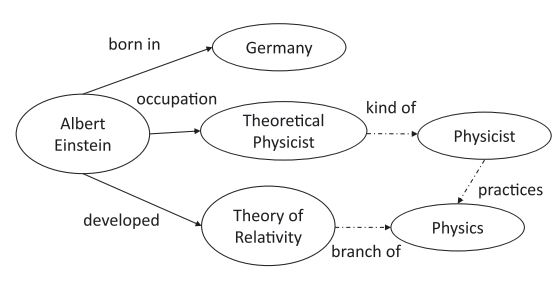
\includegraphics[width=.7\textwidth]{figures/literature-review/kg-example-albert-einstein.png}
     \rule{35em}{0.5pt}
    \caption{An example of \acrlong{kg} (\textcite{Chaudhri2022})} 
 \label{fig:kg-example-albert-einstein}
\end{figure}

\subsubsection*{Ontologies and Semantic Web Technologies}
An ontology is a formal representation of knowledge in a domain, specifying the concepts, relationships, and constraints that exist within that domain. The term ``ontology'' can be used to the shared understanding of some domain of interest \cite{Uschold1996}.
Ontologies play a critical role in defining the schema and semantics of \glspl{kg}. They specify the types of entities, relationships, and constraints, thereby providing a formalized structure for the data. The Semantic Web technologies, particularly the \gls{rdf} and the \gls{owl}, are fundamental to the development and functioning of \glspl{kg} \cite{Antoniou2008}.
\\\gls{rdf} is a standard model for data interchange on the web.
\gls{rdf} is a part of the \gls{w3c}'s Semantic Web activity and provides a model for data interchange on the Web.
It uses triples $\langle subject,predicate,object \rangle$ to represent information, providing a flexible and extensible framework for creating and managing \glspl{kg} \cite{Cyganiak14RCA}.
The subject is the resource being described, the predicate is the property or characteristic of the subject, and the object is the value of the property, that can be literals, which are concrete data values such as strings, numbers, or dates.
\gls{rdf} uses \glspl{uri} to uniquely identify subjects and predicates, ensuring that resources are globally identifiable.
\gls{rdf} can be serialized in various syntaxes, including \gls{rdf}/XML, Turtle, N-Triples, and JSON-LD. \gls{rdf}/XML is the original \gls{rdf} syntax using XML to represent \gls{rdf} triples. Turtle is a more human-readable syntax for \gls{rdf} data, concise and easier to write and read compared to \gls{rdf}/XML. N-Triples is a plain text format for encoding \gls{rdf} triples, useful for streaming data or simple data exchange. JSON-LD is a JSON-based format to serialize Linked Data, designed to be easy to use and integrate with existing JSON-based systems.

\gls{rdfs} is a semantic extension of \gls{rdf} that provides mechanisms to describe groups of related resources and the relationships between these resources. It allows for defining classes, which are categories of resources; properties, which are relationships between resources; and hierarchies, enabling inheritance.
\gls{rdf} is widely used in various domains, including the Semantic Web, where it enables the creation of a web of data with meaning, allowing machines to understand and process web content; \glspl{kg}, powering large-scale graph-based data structures used by organizations like Google and Amazon \cite{Kejriwal2022}; data integration, integrating data from disparate sources by providing a common data model; and ontology engineering, defining and using ontologies to model domain knowledge.

The \gls{owl} standard is a \gls{w3c} technology for defining and using web ontologies, enhancing \gls{rdf} by offering greater expressiveness for complex information. \gls{owl} ontologies consist of classes, properties, and individuals, enabling detailed descriptions of relationships and characteristics. It supports complex class expressions, including logical operators and restrictions like cardinality and property constraints.
\gls{owl} is used to explicitly represent the meaning of terms in vocabularies and the relationships between those terms. It enables more complex and expressive representations compared to \gls{rdfs} \cite{Deborah2004}.
\gls{owl} is used in knowledge management, information integration, and semantic search, providing a common framework for understanding and integrating data. It promotes interoperability and the creation of semantically rich, interconnected web data.

\subsubsection*{Query Languages}
\gls{sparql} is the standard query language for retrieving and manipulating data stored in \gls{rdf} format.
This query language is used to retrieve data from the GraphDB\footnote{\url{https://www.ontotext.com/products/graphdb/}} database.
It allows users to write complex queries to extract specific information from a \gls{kg}, making it a powerful tool for data analysis and knowledge discovery \cite{Jorge2009}.
It allows users to query \gls{rdf} data by specifying patterns of triples and to update \gls{rdf} data by inserting, deleting, and modifying \gls{rdf} triples. \gls{rdf} is a foundation for Linked Data, which involves interlinking data across the web using \glspl{uri} and \gls{rdf}. This enables the creation of a web of data that can be easily connected and queried.

Cypher is another query language for graph databases, such as Neo4j\footnote{\url{https://neo4j.com}}, that allows users to interact with graph data using a pattern-matching syntax. Cypher queries are used to traverse the graph, retrieve specific patterns, and perform operations on the data \cite{Francis2018}.
Cypher supports complex queries involving multiple nodes and relationships, aggregation, sorting, and limiting results. It also provides functions for working with strings, numbers, dates, and collections, as well as support for subqueries and variable-length paths.
Cypher is widely used for graph analytics, network analysis, and data exploration, enabling users to easily express complex graph traversals and operations. It leverages Neo4j's indexing and optimization capabilities to ensure efficient execution of queries, making it a powerful tool for working with connected data.

\subsection*{Applications of Knowledge Graphs}

\subsubsection*{General Applications}
\glspl{kg} have been adopted across various domains due to their ability to integrate heterogeneous data sources, provide semantic context, and enable advanced querying and reasoning.
According to \textcite{Kapanipathi2020}, in healthcare \glspl{kg} are used to integrate patient records, clinical trials, research data, and medical ontologies, enabling personalized medicine and decision support systems. They help in identifying relationships between diseases, treatments, and patient outcomes.
\\Financial institutions leverage \glspl{kg} to connect data from various sources, such as market data, regulatory information, and customer transactions. This integration facilitates risk management, fraud detection, and compliance monitoring \cite{Tchechmedjiev2019}.
\\In e-commerce, \glspl{kg} enhance product recommendation systems by linking customer preferences, purchase history, and product information. They enable more personalized and relevant recommendations, improving customer satisfaction and sales \cite{Zhang2021}.

In compliance with \textcite{Zou2020}, Fig.~\ref{fig:kg-application-fields} shows a mind map illustrating the main applications of knowledge graphs. It divides the applications into five main categories: question answering, recommendation systems, information retrieval, domain-specific applications and other applications.

\begin{figure}[htbp]
    \centering
 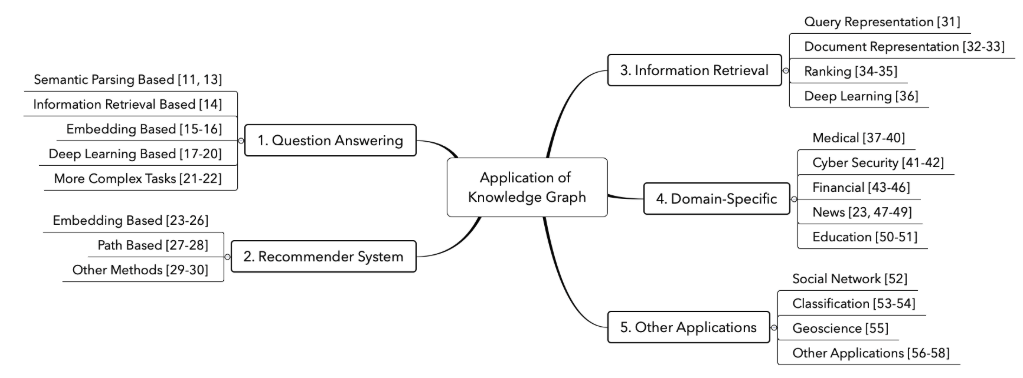
\includegraphics[width=\textwidth]{figures/literature-review/kg-application-fields.png}
     \rule{35em}{0.5pt}
    \caption{Application of \acrlongpl{kg} (\textcite{Zou2020})} 
 \label{fig:kg-application-fields}
\end{figure}

With regard to question answering, methods based on semantic parsing, methods based on information retrieval, methods based on embedding, methods based on \gls{dl} and more complex tasks are included.
\glspl{kg} significantly enhance search engines by providing semantic search capabilities. They enable the understanding of user queries in context, allowing for more accurate and relevant search results. Google's Knowledge Graph is a prominent example, enhancing search results with information about entities and their relationships \cite{singhal2012introducing}.
Recommender systems are classified into embedding-based methods, path-based methods and other methods. Information retrieval includes query representation, document representation, ranking and \gls{dl}. Domain-specific applications include medicine, computer security, finance, news and education.
Within enterprises, \glspl{kg} are used to manage and utilize internal knowledge effectively. They integrate data from different departments, such as human resources, finance, and operations, providing a unified view of the organization's information. This integration supports decision-making, collaboration, and innovation \cite{pujara2013knowledge}.
Other applications include social networks, classification, geosciences and various other applications.


\subsection*{Recent Advancements in Knowledge Graphs}

\subsubsection*{Integration with Machine Learning}
Recent research has focused on integrating \glspl{kg} with \gls{ml} and \gls{dl} techniques to enhance their capabilities and applications. These integrations have led to significant advancements in various areas, including \gls{nlp}, recommendation systems, and predictive analytics.

\glspl{kge}: \gls{kge} techniques represent entities and relationships in a continuous vector space, enabling the use of \gls{ml} algorithms for tasks such as link prediction, entity classification, and clustering. Popular methods include TransE \cite{Bordes2013}, TransH \cite{Wang2014}, and TransR \cite{Lin2015}, each providing different ways to model relationships in the embedding space \cite{Wang2017}.

\glspl{gnn}: \glspl{gnn} are \gls{dl} models designed to operate on graph-structured data. They leverage the relational nature of graphs to perform tasks such as node classification, link prediction, and graph classification. \glspl{gnn} have been successfully applied to enhance the capabilities of \glspl{kg} in various domains \cite{Wu2021}.

\subsubsection*{Natural Language Processing and Question Answering}
\glspl{kg} have been instrumental in advancing \gls{nlp} applications, particularly in question answering systems. By providing structured and semantically rich information, \glspl{kg} enable systems to understand and generate human language more effectively.
\glspl{kg} support question answering systems by enabling them to retrieve and reason over structured data.
These systems can answer complex queries by traversing the graph and applying logical inferences based on the relationships between entities \cite{Yasunaga2021}.
\glspl{kg} enhance text analysis and semantic search by providing contextual information about entities mentioned in the text.
This contextual understanding improves the accuracy of information retrieval and the relevance of search results \cite{Fernandez2011}.

\subsection*{Well-Known Knowledge Graphs and Ontologies in Research Field}
Well-known \glspl{kg} and ontologies have significantly influenced the research field by providing structured representations of knowledge that facilitate data integration, retrieval, and analysis.
One prominent example was the \gls{mag}, a comprehensive dataset that mapped scholarly publications, authors, institutions, and topics, enabling advanced research trend analysis and collaboration discovery \cite{Wang2020}.
Although \gls{mag} was discontinued in 2021 as Microsoft shifted its focus to supporting open academic initiatives, its legacy lives on through platforms like OpenAlex, a successor to \gls{mag} that serves as an open-source resource connecting entities such as authors, publications, and journals with detailed metadata \cite{priem2022}.

\begin{figure}[htbp]
    \centering
 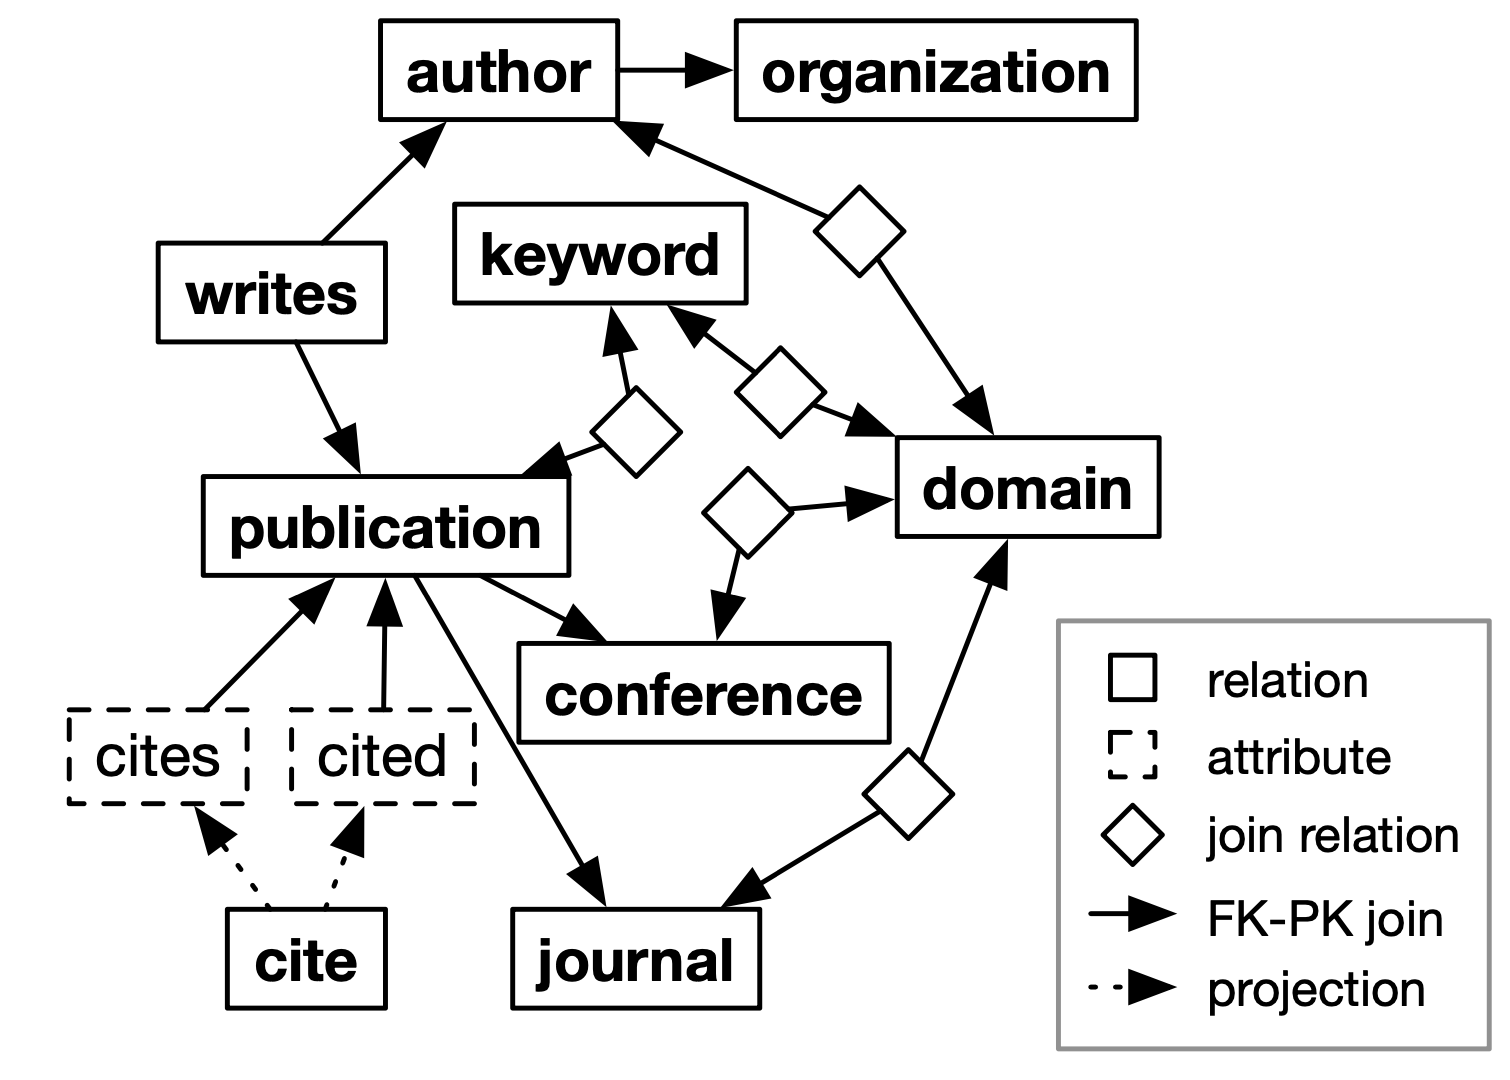
\includegraphics[width=0.8\textwidth]{figures/literature-review/mag-schema.png}
     \rule{35em}{0.5pt}
    \caption{A simplified version of the \gls{mag} Search database's schema (\textcite{Baik2019})} 
 \label{fig:mag-schema}
\end{figure}

Another essential resource is the the \gls{s2ag}, developed by the Allen Institute for \acrlong{ai}, represents one of the most extensive and advanced knowledge graphs in the research domain \cite{S2AG}.
\gls{s2ag} contains over 205 million publications, 121 million authors, and nearly 2.5 billion citation edges, making it a powerful resource for understanding and analyzing academic networks.
By integrating metadata from sources such as Crossref, PubMed, and Unpaywall, and processing nearly 60 million full-text publications, \gls{s2ag} enables rich insights into scholarly communication.
The data is accessible through public APIs and downloadable snapshots, fostering applications in natural language processing, citation analysis, and research trend discovery.
\gls{s2ag} exemplifies the potential of \glspl{kg} to address information overload by enabling efficient discovery of relevant research literature.
Its availability as an open resource highlights the growing emphasis on open science and collaborative innovation in the academic community.

Wikidata is a collaboratively edited \gls{kg} that serves as a centralized data repository for structured information across various domains, supporting Wikimedia projects like Wikipedia and numerous external applications \cite{Wikidata2014}.
Introduced in 2012 by the Wikimedia Foundation, Wikidata provides a platform where entities, such as people, places, events, and concepts, are represented as items with unique identifiers.
These items are described using statements, which consist of properties and values, forming a triple-based structure similar to other semantic web technologies.
One of the most distinguishing features of Wikidata is its adherence to the principles of \gls{lod}.
It allows the integration with other \glspl{kg} and ontologies by supporting globally recognized identifiers, such as \glspl{doi}, \glspl{orcid}, and \gls{viaf} IDs, and linking to external datasets.
This capability makes it a valuable resource for connecting fragmented knowledge across the web.
The Wikidata \gls{kg} is highly dynamic and continuously enriched by a global community of contributors and automated tools like bots.
Its multilingual support ensures accessibility to a diverse audience.
Applications of Wikidata include natural language processing, recommendation systems, semantic search, and research in \gls{ai}.
Due to its openness, flexibility, and integration capabilities, Wikidata is increasingly being adopted as a foundational resource for creating and enriching domain-specific knowledge graphs, supporting scholarly projects, and powering data-driven insights.

Furthermore, the \gls{orkg} offers a dynamic, semantic representation of research contributions, focusing on contextualizing findings within their scientific domain to support comparative studies and systematic reviews \cite{ORKG}.
The \gls{orkg} aims to address the challenge of information overload in scholarly research by structuring and presenting scientific knowledge in a machine-readable format.
Unlike traditional research dissemination approaches, which rely on static publications, the \gls{orkg} provides a platform for collaboratively curating research content with semantically rich metadata, enabling advanced analysis and discovery.
Through the use of \gls{lod} principles and Semantic Web technologies, the \gls{orkg} facilitates the comparison of research findings across studies by aligning key concepts, methodologies, and outcomes.
This structured representation allows researchers to identify gaps in the literature, reproduce experiments, and generate new insights with greater efficiency.
The platform also supports automated reasoning and \gls{ai}-driven tools, making it easier to navigate large volumes of data and extract relevant patterns or trends.
The \gls{orkg} is particularly valuable for interdisciplinary research, where integrating knowledge from multiple domains is essential.
By linking related studies and establishing semantic connections between concepts, the \gls{orkg} enhances the accessibility and usability of scientific knowledge for both humans and machines.
This approach not only accelerates scientific progress but also lays the groundwork for the next generation of research infrastructures.

The VIVO Ontology, which forms the core of the VIVO platform and is designed to represent scholarly activity in a structured and interoperable manner \cite{VIVO}.
It emphasizes the use of semantic technologies such as \gls{rdf} and \gls{owl} to model relationships among academic entities like researchers, publications, grants, and institutions.
By employing these standards, the ontology enables data to be expressed in a machine-readable format as triples, which facilitates reasoning, integration, and discovery.

\begin{figure}[htbp]
    \centering
 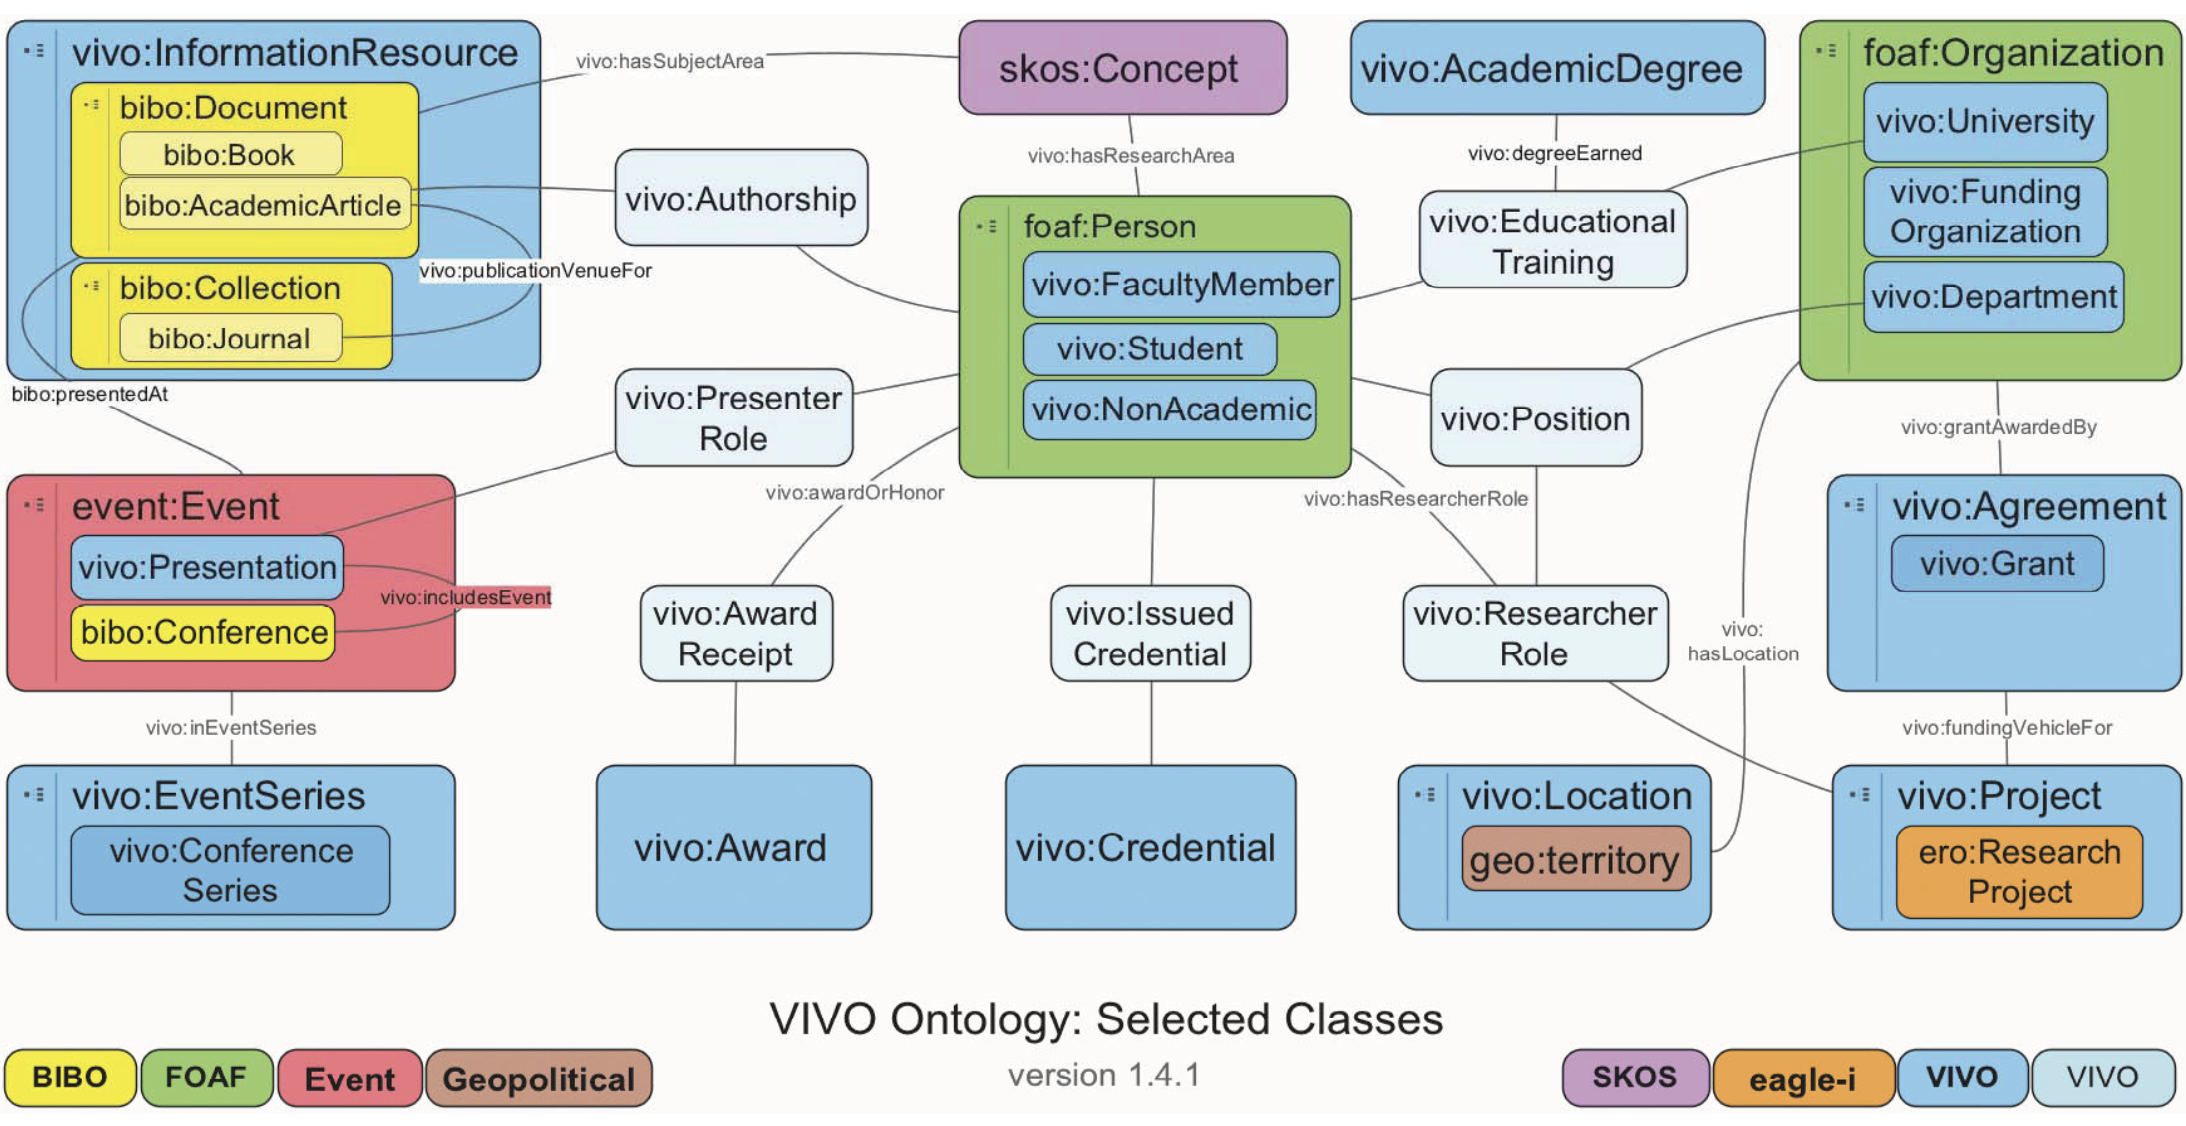
\includegraphics[width=0.8\textwidth]{figures/literature-review/vivo-ontology.png}
     \rule{35em}{0.5pt}
    \caption{Key classes in the VIVO ontology are highlighted alongside their source ontologies, with ``context nodes'' (depicted in light blue) providing temporal details and other information specific to individual relationships. (\textcite{VIVO})}
 \label{fig:vivo-ontology}
\end{figure}

The design of the VIVO Ontology is guided by clear goals, including the ability to represent complex academic relationships and maintain independence from specific implementations to ensure adaptability across diverse institutional contexts.
A hierarchical class structure is employed to define scholarly entities, with an emphasis on modularity and scalability to accommodate the evolving needs of the academic community.
Additionally, the ontology supports the use of external controlled vocabularies and common identifiers to enhance data consistency and interoperability with other systems.

VIVO leverages several well-established ontologies, such as \gls{foaf}, to enrich its representation of scholarly data and ensure interoperability with other systems.
\gls{foaf} is a widely-used ontology designed to describe people, their activities, and their relationships to other people and objects.
The core element of a \gls{foaf} document is the \gls{foaf} vocabulary, which is defined by the namespace: \textless http://xmlns.com/foaf/0.1/\textgreater.
By integrating \gls{foaf}, VIVO can represent entities like researchers and their social networks, enabling a consistent and standard framework for modeling relationships such as collaborations, affiliations, and connections to digital artifacts like websites or profiles.
The primary reason VIVO uses \gls{foaf} is to adopt existing, well-defined vocabularies rather than reinventing the wheel, which promotes interoperability across systems and facilitates data sharing on the Semantic Web.
\gls{foaf}'s compatibility with \gls{lod} principles allows VIVO to easily connect its data with external resources, enhancing discoverability and integration.
For example, \gls{foaf}'s properties such as foaf:Person and foaf:knows align perfectly with VIVO's requirements for describing researchers and their relationships, while maintaining compliance with Semantic Web standards.
By utilizing external ontologies like \gls{foaf}, VIVO not only achieves a more robust and extensible data model but also ensures that its ontology can interact with broader data ecosystems, advancing the goal of creating a globally connected research information infrastructure.
This strategic reuse of established ontologies supports VIVO's vision of openness, interoperability, and scalability in scholarly networking and discovery.
The VIVO Ontology serves as the core of the VIVO application, functioning as a data model and enabling reasoning to infer new relationships based on existing data.
Its flexibility allows institutions to extend the ontology to meet specific local requirements while adhering to its core principles, thereby maintaining compatibility with the broader VIVO ecosystem.
Community-driven efforts play a crucial role in the continuous refinement and expansion of the ontology, ensuring its relevance and alignment with advancements in academic practices.
By supporting the creation of \gls{lod}, the VIVO Ontology facilitates improved research discovery, expert identification, and collaboration across institutions.
%
\section{Large Language Models}\label{sec:large-language-models}
\glspl{llm} have emerged as a transformative innovation in \gls{nlp}, leveraging \gls{dl} techniques to understand, generate, and manipulate human language with unprecedented accuracy.
Fig.~\ref{fig:llms-over-the-years} shows the increasing trend in the number of \glspl{llm} releases and the names of some significant \glspl{llm} proposed from 2019 to 2024.

\begin{figure}[htbp]
    \centering
 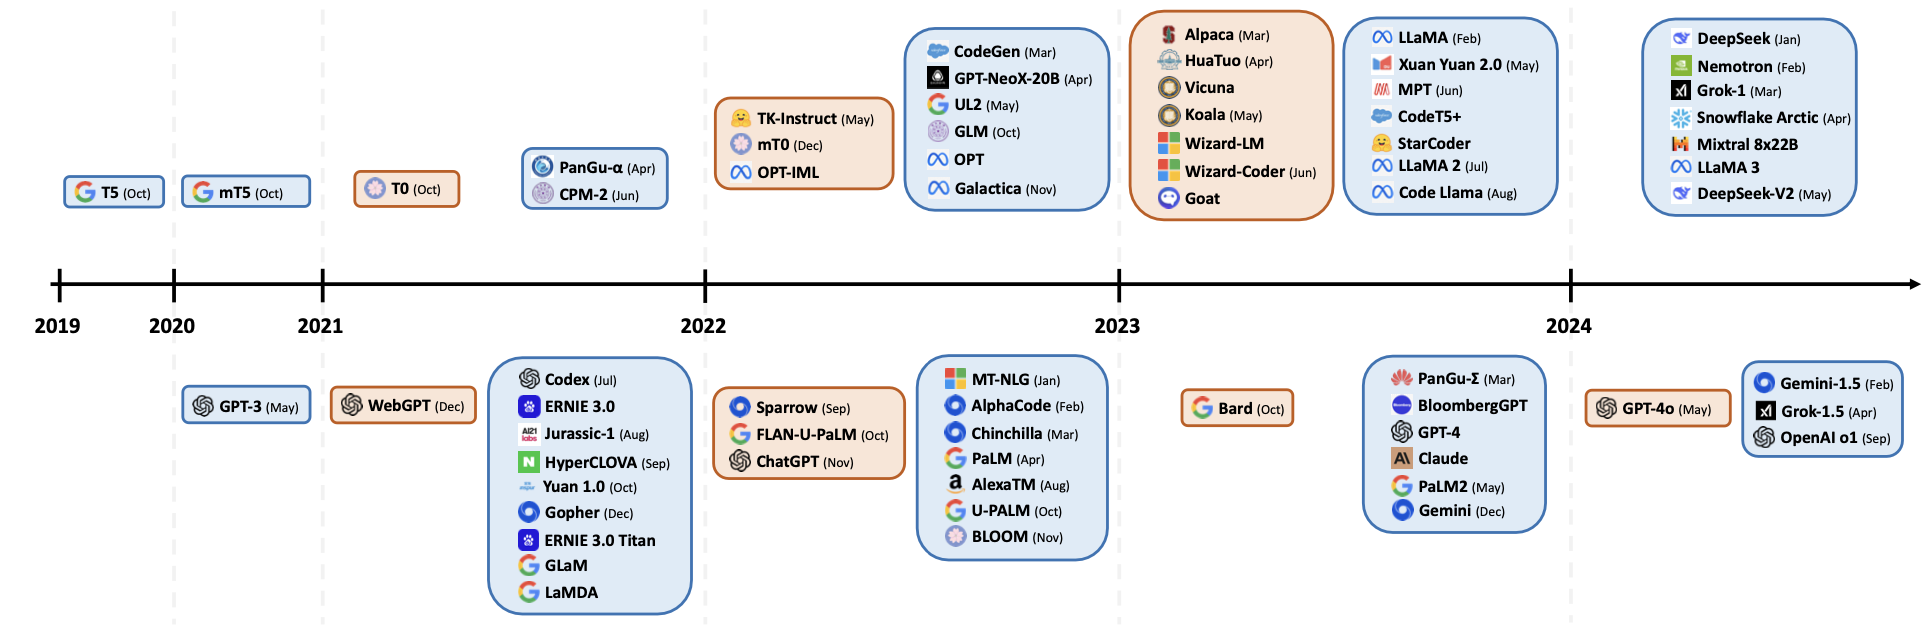
\includegraphics[width=\textwidth]{figures/literature-review/llms-over-the-years.png}
     \rule{35em}{0.5pt}
    \caption{Timeline of \gls{llm} releases: blue cards represent pre-trained models, orange cards denote instruction-tuned models. Open-source models appear on the top, while closed-source models are on the bottom, showing the shift toward open-source and instruction-tuned trends. (\textcite{Naveed2023})}
 \label{fig:llms-over-the-years}
\end{figure}

\glspl{llm}, such as OpenAI's GPT series \cite{Radford2018ImprovingLU}, Google's BERT \cite{Devlin2019BERTPO}, and more recent iterations like GPT-4, are typically built on transformer architectures \cite{Vaswani2017}.
The transformer model introduced a self-attention mechanism that efficiently captures contextual relationships between words across large textual sequences, overcoming limitations of earlier models like \glspl{rnn} and \glspl{lstm} in handling long-range dependencies.
These models are pre-trained on massive corpora containing diverse text from books, articles, and web sources, allowing them to generalize linguistic patterns, syntax, semantics, and even factual knowledge embedded in the data.
According to \textcite{Chang2024}, \glspl{llm} perform a wide range of tasks in \gls{nlp}, often achieving state-of-the-art results across various benchmarks.
Fig.~\ref{fig:llms-overview} provides a broader overview of the organization of \glspl{llm}, categorizing them into seven distinct branches: pre-training, fine-tuning, efficiency, inference, evaluation, applications, and challenges.
These branches reflect the key aspects of the development, deployment, and evaluation of \glspl{llm}.
Pre-training focuses on the foundational step of training models on vast, diverse corpora to learn language representations.
Fine-tuning involves adapting pre-trained models for specific tasks, enhancing their performance on downstream applications.
Efficiency addresses the computational and energy requirements of training and deploying \glspl{llm}, emphasizing methods like parameter-efficient tuning and pruning to reduce resource consumption.
The inference branch examines the process of generating outputs from trained models, focusing on optimizing speed and accuracy.
More advanced capabilities, such as few-shot and zero-shot learning, enable \glspl{llm} to adapt to new tasks with minimal to no task-specific training data, a feature prominently demonstrated by GPT-3 \cite{NEURIPS2020_1457c0d6}.
Evaluation highlights the metrics and benchmarks used to assess \glspl{llm}' performance on various tasks, ensuring they meet quality standards.
Applications span the diverse real-world use cases of \glspl{llm}, from natural language understanding to robotics and multi-modal systems.
Finally, challenges encompass the limitations and issues of \glspl{llm}, including bias, hallucination, and environmental impact, offering directions for future research and improvement.
These branches collectively define the lifecycle and scope of advancements in \glspl{llm} research, providing a comprehensive framework for understanding their capabilities and impact.

\begin{figure}[htbp]
    \centering
 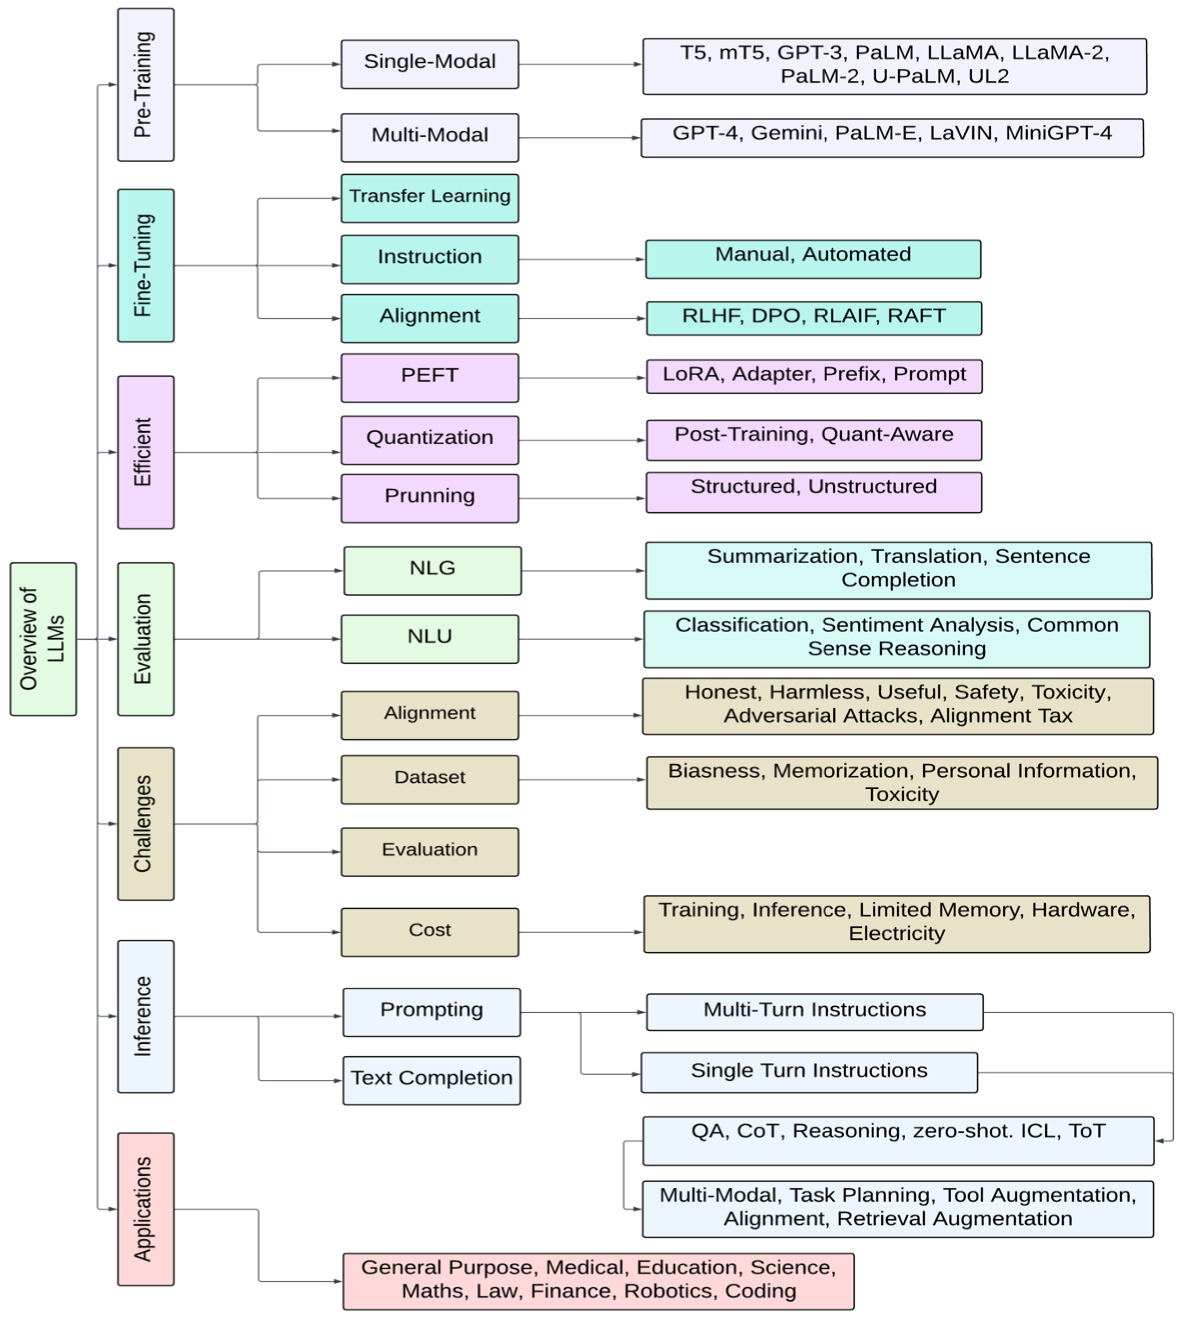
\includegraphics[width=0.8\textwidth]{figures/literature-review/llms-overview.png}
     \rule{35em}{0.5pt}
    \caption{An overview of \glspl{llm} divided into seven branches: pre-training, fine-tuning, efficiency, evaluation, challenges, inference, and applications. (\textcite{Naveed2023})}
 \label{fig:llms-overview}
\end{figure}

This adaptability has made \glspl{llm} suitable for tasks requiring contextual reasoning, dialogue systems, and even code generation, as seen in models like Codex \cite{Chen2021EvaluatingLL}, which powers tools such as GitHub Copilot\footnote{\url{https://github.com/features/copilot}}.
The applications of \glspl{llm} span numerous domains, reflecting their versatility and broad impact.
In industry, \glspl{llm} power conversational agents, customer service bots, and content creation tools.
In research and education, they facilitate automated summarization of scientific literature, personalized tutoring, and question-answering systems to support knowledge discovery.
The integration of \glspl{llm} with domain-specific knowledge graphs and ontologies further enhances their reliability, particularly in specialized areas such as medicine, law, and scientific discovery \cite{Yang2024}.
Despite their strengths, \glspl{llm} have some limitations.
One important problem is their dependence on vast computational resources for training, which has implications for environmental sustainability \cite{Strubell2019EnergyAP}.
Furthermore, \glspl{llm} tend to propagate biases present in the training data, leading to inconsistencies when deployed in real-world applications \cite{Naveed2023}.
They also suffer from factual inaccuracies and hallucinations, where the model generates plausible yet incorrect information \cite{Chang2024}, which limits their applicability in high-stakes environments requiring factual precision.
Moreover, the lack of interpretability in \glspl{llm} remains a significant challenge, as their outputs are generated from complex internal representations that are not easily explainable, leading to questions about trust and accountability \cite{Naveed2023}.
Nevertheless, the advantages of \glspl{llm} are substantial, as they offer unprecedented performance in language-related tasks, significant generalizability, and the ability to operate across diverse applications without extensive task-specific engineering.
In their study, \textcite{Naveed2023} discuss that current research about \glspl{llm} efforts are focused on addressing their limitations, particularly improving energy efficiency, reducing bias, enhancing factual accuracy, and developing methods for better interpretability.
As \glspl{llm} continue to evolve, their integration with structured knowledge systems and advancements in alignment with human intent are likely to redefine their role in solving complex problems across industries.
%
\section{Retrieval-Augmented Generation}\label{sec:retrieval-augmented-generation}
\acrfull{rag} improves \glspl{llm} by integrating real-time data retrieval into the generative process \cite{singh2025}.
Unlike static \glspl{llm} that rely on pre-trained knowledge, \gls{rag} dynamically retrieves relevant external information, improving response accuracy, contextual relevance and updateability \cite{Fan2024, singh2025}.

\begin{figure}[htbp]
  \centering
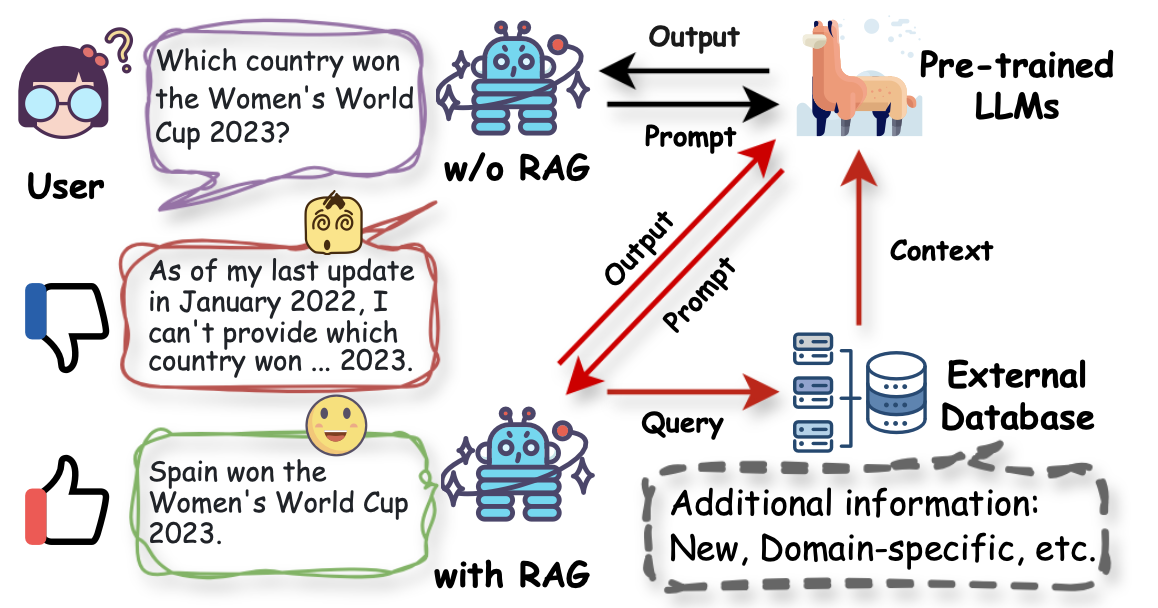
\includegraphics[width=.7\textwidth]{figures/literature-review/rag-no-rag-example.png}
   \rule{35em}{0.5pt}
  \caption{An example of the limitations of \glspl{llm} without retrieval mechanisms (top) and the benefits of \gls{rag} with real-time data retrieval (bottom) (\textcite{Fan2024})}
\label{fig:rag-no-rag-example}
\end{figure}

When a user's query requires information beyond the training data of a \gls{llm}, such as real-time knowledge or unseen facts, the model's response may be outdated or incomplete.
In such cases, standard \glspl{llm} without external retrieval mechanisms struggle to provide accurate answers, as illustrated in the upper part of the Fig.~\ref{fig:rag-no-rag-example}.
Here, the model fails to answer a simple fact-based question about the winner of the 2023 Women's World Cup due to its training data cutoff.
However, with \gls{rag}, as shown in the lower part of the image, the system retrieves relevant information from an external database before generating a response.
This enables the model to produce up-to-date and contextually accurate answers by grounding its output in real-world knowledge.
Fig.~\ref{fig:rag-components} shows the three main components of \gls{rag}:
\begin{itemize}
    \item \textbf{Retrieval}: queries external sources such as knowledge bases, APIs or vector databases, using dense vector search and advanced transformer-based models to improve accuracy.
    \item \textbf{Augmentation}: processes, extracts and synthesises the retrieved data to align it with the user's query.
    \item \textbf{Generation}: combines the retrieved information with the \gls{llm}'s internal knowledge to produce coherent and contextually relevant answers. 
\end{itemize}
	
\begin{figure}[htbp]
    \centering
 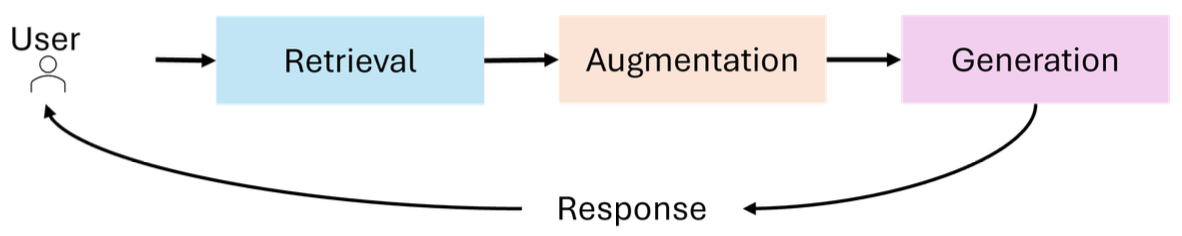
\includegraphics[width=.65\textwidth]{figures/literature-review/RAGcomponents.png}
     \rule{35em}{0.5pt}
    \caption{\gls{rag} components (\textcite{singh2025})}
 \label{fig:rag-components}
\end{figure}

The evolution of \gls{rag} has given rise to several paradigms, each of which refines the interaction between retrieval and generation to improve contextual accuracy, scalability and reasoning capabilities.
From the basic Na\"ive \gls{rag} to the more sophisticated Advanced \gls{rag}, Modular \gls{rag} and Graph\gls{rag}, these approaches have progressively addressed major limitations.
The newest and most powerful paradigm, Agentic \gls{rag}, introduces autonomous agents that dynamically adapt retrieval strategies, optimise workflows and enable complex multi-stage reasoning.
Each paradigm is briefly described in the next subsections.
Table~\ref{table:rag-paradigms-comparison} provides a comparison of the key features, strengths and challenges of these \gls{rag} paradigms.

\subsection*{Na\"ive \gls{rag}}\label{sec:naive-rag}
Na\"ive \gls{rag} is the most fundamental implementation of \gls{rag}, characterized by a straightforward retrieve-read framework \cite{gao_retrieval-augmented_2024}.
It consists of three main steps: indexing, retrieval, and generation \cite{gao_retrieval-augmented_2024,singh2025}.
During indexing, raw data from various sources (e.g., PDFs, Word documents, HTML) is cleaned, segmented into smaller text chunks, and embedded into a vector representation using an embedding model before being stored in a vector database.
When a user poses a query, the system retrieves the most relevant text chunks based on semantic similarity using the same embedding model.
These retrieved chunks are then incorporated into the generation phase, where a \gls{llm} synthesizes a response using both the retrieved information and its internal knowledge.
While Na\"ive \gls{rag} effectively enhances \glspl{llm} by integrating external knowledge, it suffers from several limitations, described as follows.
Retrieval inefficiencies: the retrieved chunks may be irrelevant, misaligned, or miss crucial context, reducing the quality of responses \cite{gao_retrieval-augmented_2024,singh2025}.
Hallucinations: the \gls{llm} may generate content unsupported by retrieved data, leading to factual inaccuracies \cite{gao_retrieval-augmented_2024}.
Redundancy and inconsistency: retrieved information may be overlapping or disjointed, making it challenging to generate coherent answers \cite{gao_retrieval-augmented_2024}.
Limited adaptability: a single retrieval pass based on the original query might not capture sufficient context, restricting performance in complex tasks \cite{gao_retrieval-augmented_2024,singh2025}.
Despite its simplicity, Na\"ive \gls{rag} provided the foundation for more advanced \gls{rag} paradigms, such as Advanced \gls{rag} and Modular \gls{rag}, which introduce retrieval optimization, re-ranking mechanisms, and multi-step reasoning to address these challenges.

\subsection*{Advanced \gls{rag}}\label{sec:advanced-rag}
Advanced \gls{rag} enhances the limitations of Na\"ive \gls{rag} by integrating sophisticated retrieval optimization techniques and semantic understanding to improve information retrieval and generation quality \cite{gao_retrieval-augmented_2024}.
Unlike Na\"ive \gls{rag}, which relies on simple keyword-based retrieval, Advanced \gls{rag} employs \gls{dpr} \cite{Karpukhin2020} and neural ranking algorithms to prioritize relevant information \cite{singh2025}.
It introduces pre-retrieval optimizations such as query expansion, metadata enrichment, and indexing improvements to refine the quality of retrieved data.
Additionally, it implements post-retrieval techniques like context re-ranking, summarization, and adaptive filtering, ensuring that the retrieved information aligns more effectively with the user query before being fed into the language model.
Furthermore, Advanced \gls{rag} supports multi-hop retrieval, allowing the system to retrieve and combine insights from multiple sources to generate well-informed and contextually aware responses.
These enhancements make it more scalable and precise, making it well-suited for knowledge-intensive applications such as scientific research, legal reasoning, and enterprise search solutions.
However, it comes with challenges such as higher computational overhead and latency due to complex retrieval and ranking processes.

\subsection*{Modular \gls{rag}}\label{sec:modular-rag}
Modular \gls{rag} addresses the limitations of Na\"ive and Advanced \gls{rag} by incorporating flexible and composable components, enabling greater adaptability and optimization for specific use cases \cite{gao_retrieval-augmented_2024}.
In contrast to the linear pipeline of traditional \gls{rag}, Modular \gls{rag} enables independent modification and replacement of retrieval, augmentation, and generation modules, making it highly customizable.
According to \cite{singh2025}, key enhancements include hybrid retrieval strategies, where both sparse (e.g., BM25) and dense retrieval \cite{Karpukhin2020} (e.g., \gls{dpr}) techniques are combined for better query matching, and multi-source retrieval, which integrates structured (databases, \glspl{kg}) and unstructured (documents, APIs) sources.
Moreover, modular \gls{rag} introduces new modules like adaptive search, memory, and task-specific adapters, along with new patterns such as iterative retrieval and dynamic module reconfiguration, enhancing flexibility and precision across diverse applications \cite{gao_retrieval-augmented_2024}.
It also supports dynamic query rewriting and multi-step reasoning, allowing iterative refinements to retrieval results.
Its modular design makes it ideal for domain-specific tasks, such as financial analytics and scientific research, where different retrieval and augmentation techniques are needed.
However, this paradigm faces challenges in complex data integration, requiring handling of unstructured, semi-structured, and structured data; system orchestration, demanding precise workflow management across modular components; and component selection and optimization, ensuring individual modules are fine-tuned and effectively integrated for optimal performance.
Fig.~\ref{fig:naive-advanced-modular-rag} illustrates the three \gls{rag} paradigms just described, Na\"ive, Advanced and Modular \gls{rag}, highlighting their key components, optimisations and structural differences.
\begin{figure}[htbp]
    \centering
 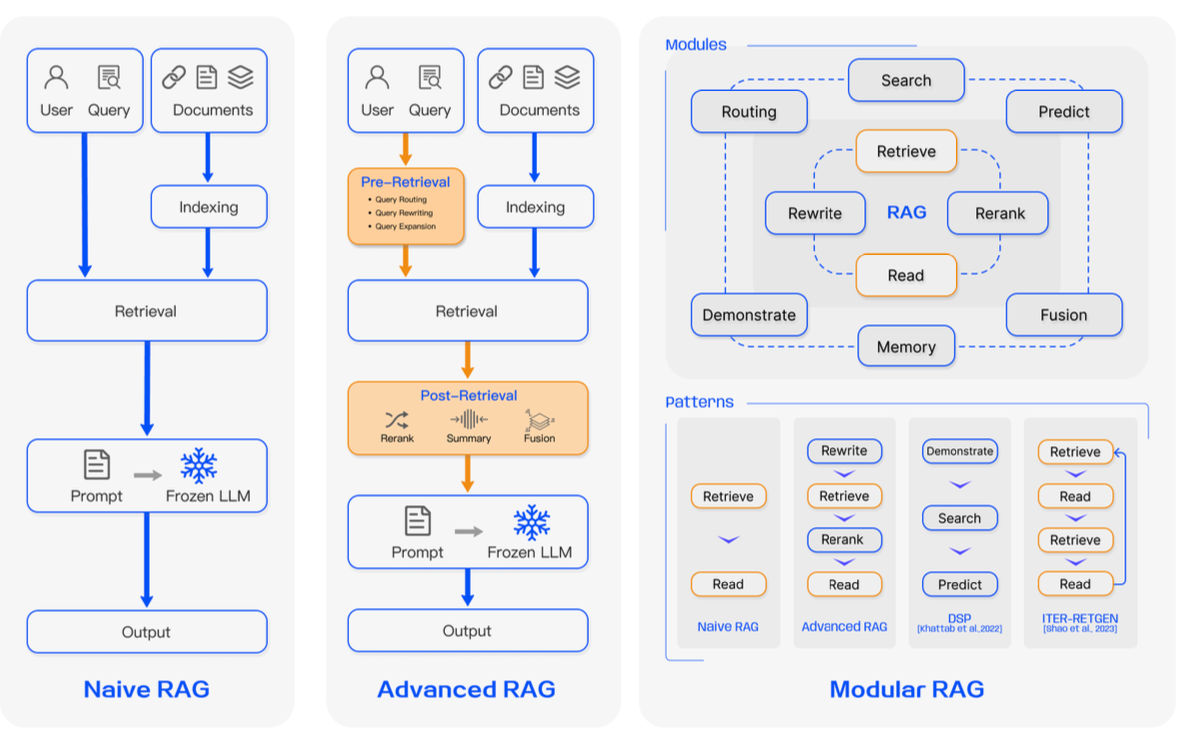
\includegraphics[width=.75\textwidth]{figures/literature-review/naive-advanced-modular-rag.png}
     \rule{35em}{0.5pt}
    \caption{Na\"ive, Advanced and Modular \gls{rag} architectures (\textcite{gao_retrieval-augmented_2024})}
 \label{fig:naive-advanced-modular-rag}
\end{figure}

\subsection*{Graph\gls{rag}}\label{sec:graph-rag}
Graph\gls{rag} is an advanced \gls{rag} framework that leverages structured \glspl{kg}, as illustrated in Fig.~\ref{fig:graph-rag-architecture} , to improve contextual understanding and response generation by \glspl{llm} \cite{peng2024graphragsurvey,singh2025}.
Unlike traditional \gls{rag} approaches that rely solely on retrieving textual information, Graph\gls{rag} incorporates relational knowledge by retrieving structured graph elements, such as nodes, triples, paths, or subgraphs, from a pre-constructed graph database.
This allows for more accurate and context-aware responses, as it captures entity relationships that text-based methods often overlook \cite{singh2025}.
One of the key distinctions between Graph\gls{rag} and standard \gls{rag} is its ability to maintain and utilize explicit structural connections, whereas text-based \gls{rag} primarily depends on similarity-based retrieval from unstructured text corpora.
Graph\gls{rag} thus reduces redundancy and enhances global information retrieval by abstracting and summarizing textual data into a more structured form.
Among its advantages, Graph\gls{rag} enables more precise and comprehensive retrieval, effectively capturing relational knowledge that improves factual consistency and mitigates hallucination.
Additionally, it facilitates query-focused summarization by retrieving subgraphs that include broader contextual information, reducing verbosity in responses.
However, Graph\gls{rag} also presents limitations, including scalability challenges due to the exponential growth of subgraph candidates and the dependency on high-quality, well-structured graph data \cite{singh2025}.
Integrating graph-based retrieval with unstructured retrieval mechanisms adds complexity to implementation, making Graph\gls{rag} more computationally demanding than traditional \gls{rag} approaches \cite{peng2024graphragsurvey,singh2025}.

\begin{figure}[htbp]
    \centering
 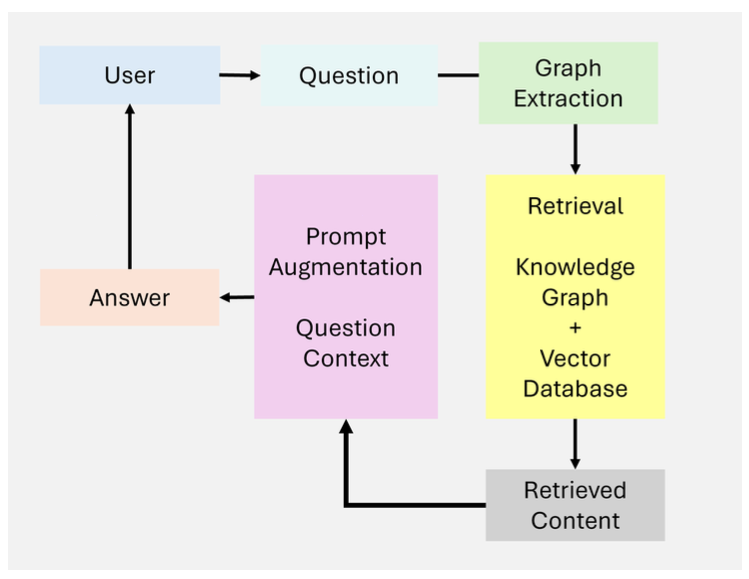
\includegraphics[width=.65\textwidth]{figures/literature-review/graphRAG.png}
     \rule{35em}{0.5pt}
    \caption{Graph\gls{rag} architecture (\textcite{singh2025})}
 \label{fig:graph-rag-architecture}
\end{figure}

\subsection*{Agentic \gls{rag}}\label{sec:agentic-rag}
Agentic\gls{rag} extends traditional \gls{rag} frameworks by integrating autonomous agents that dynamically manage retrieval, reasoning, and response generation workflows \cite{singh2025}.
Unlike standard \gls{rag} systems, which rely on predefined retrieval pipelines, Agentic\gls{rag} incorporates agentic design patterns such as reflection, planning, tool use, and multi-agent collaboration to enable adaptive decision-making and iterative refinement.
These autonomous agents assess query complexity, refine search strategies, and optimize knowledge integration, leading to improved contextual accuracy and scalability.
A key advantage of Agentic\gls{rag} is its ability to manage multi-step reasoning processes, allowing for more precise responses to complex queries.
By dynamically orchestrating workflows, these systems enhance retrieval efficiency and minimize hallucinations by iteratively validating retrieved content.
However, the increased complexity of Agentic\gls{rag} poses challenges, including higher computational overhead and the need for sophisticated coordination mechanisms among multiple agents.
An example of a Multi-Agent Agentic\gls{rag} architecture is shown in Fig.~\ref{fig:multi-agent-agentic-rag}.
Additionally, while it improves adaptability, the unpredictability of agent-driven workflows can introduce variability in response generation.
Despite these challenges, Agentic\gls{rag} is particularly well-suited for domains requiring dynamic adaptability, such as financial analytics, healthcare diagnostics, and legal research, where multi-agent collaboration and iterative refinement enhance the reliability of \gls{ai}-generated insights \cite{singh2025}.

\begin{figure}[htbp]
    \centering
 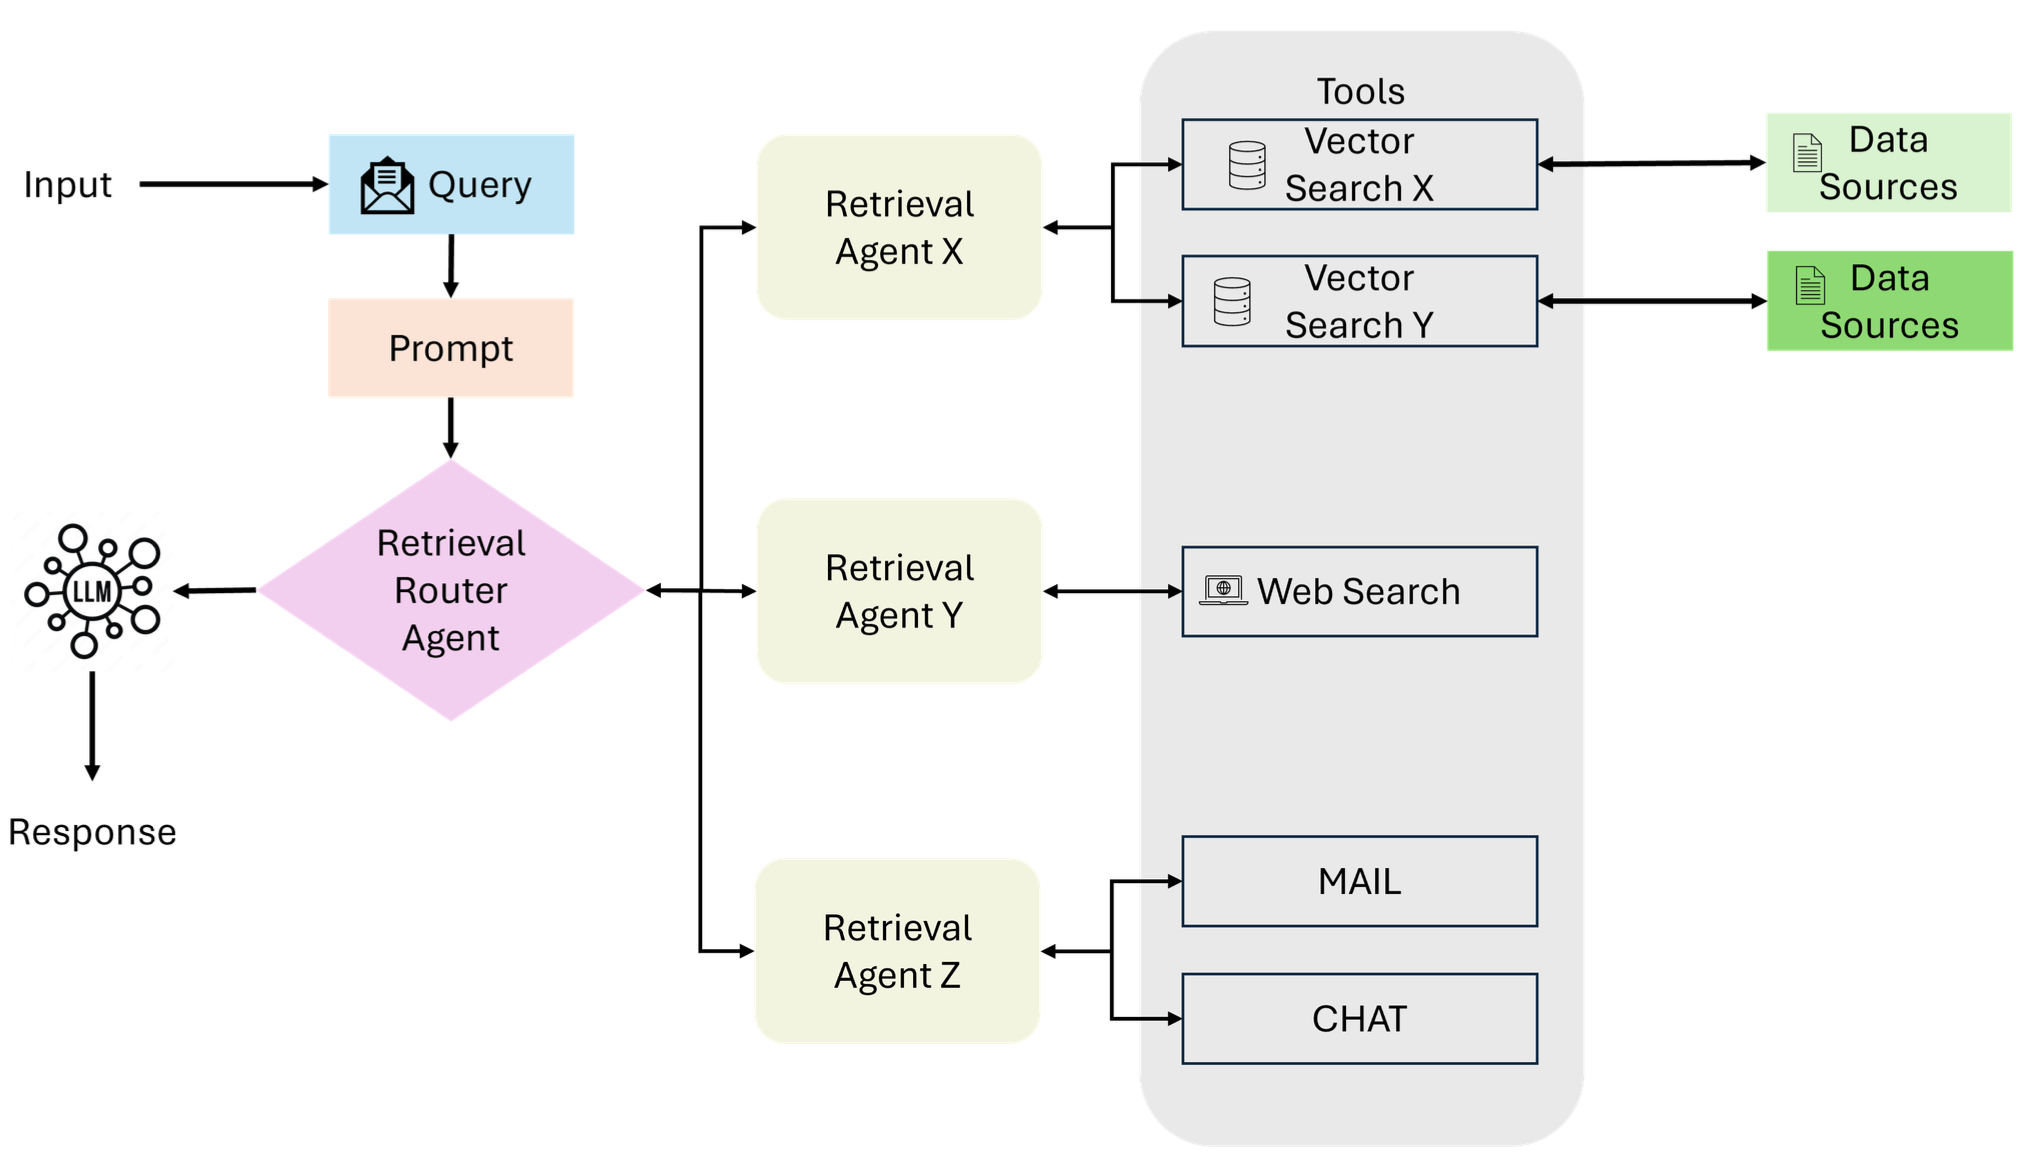
\includegraphics[width=.8\textwidth]{figures/literature-review/multi-agent-agentic-rag.png}
     \rule{35em}{0.5pt}
    \caption{Multi-Agent Agentic\gls{rag} architecture (\textcite{singh2025})}
 \label{fig:multi-agent-agentic-rag}
\end{figure}

\begin{table}[htbp]
    \centering
    \scriptsize
    \begin{tabularx}{\textwidth}{|>{\centering\arraybackslash}p{1.5cm}|X|X|X|}
      \hline
      \textbf{\gls{rag} Paradigm} & \textbf{Key Features} & \textbf{Strengths} & \textbf{Challenges}\\
      \hline
          \begin{center}
            Na\"ive
          \end{center} & \begin{itemize}[nosep, left=0pt]
        \item Keyword-based retrieval (e.g., TF-IDF, BM25)
      \end{itemize} & \begin{itemize}[nosep, left=0pt]
        \item Simple and easy to implement
        \item Suitable for fact-based queries
      \end{itemize}& \begin{itemize}[nosep, left=0pt]
        \item Retrieval inefficiency
        \item Hallucinations
        \item Redundancy and inconsistency
        \item Limited adaptability
      \end{itemize}\\
      \hline
      \begin{center}
      Advanced
      \end{center} & \begin{itemize}[nosep, left=0pt]
        \item Dense retrieval models (e.g., DPR)
        \item Neural ranking and re-ranking
        \item Multi-hop retrieval
      \end{itemize} & \begin{itemize}[nosep, left=0pt]
        \item High precision retrieval
        \item Improved contextual relevance
      \end{itemize} & \begin{itemize}[nosep, left=0pt]
        \item Higher computational overhead
        \item Latency
      \end{itemize}\\
      \hline
      \begin{center}
        Modular
      \end{center} & \begin{itemize}[nosep, left=0pt]
        \item Hybrid retrieval (sparse and dense)
        \item Tool and API integration
        \item Composable, domain-specific pipelines
      \end{itemize} & \begin{itemize}[nosep, left=0pt]
        \item High flexibility and customization
        \item Suitable for diverse applications
        \item Scalable
      \end{itemize} & \begin{itemize}[nosep, left=0pt]
        \item Complex data integration
        \item System orchestration and workflow management
        \item Component selection and optimization
        \item Maintenance
      \end{itemize}\\
      \hline
      \begin{center}
        Graph
      \end{center} & \begin{itemize}[nosep, left=0pt]
        \item Integration of graph-based structures
        \item Multi-hop reasoning
        \item Contextual enrichment via nodes
      \end{itemize}& \begin{itemize}[nosep, left=0pt]
        \item Relational reasoning capabilities
        \item Mitigates hallucinations
        \item Ideal for structured data tasks
      \end{itemize}& \begin{itemize}[nosep, left=0pt]
        \item Scalability challenges
        \item Dependency on high-quality graph data
        \item Complexity of integration
      \end{itemize}\\
      \hline
      \begin{center}
        Agentic
      \end{center} & \begin{itemize}[nosep, left=0pt]
        \item Autonomous agents
        \item Dynamic decision-making
        \item Iterative refinement and workflow optimization
      \end{itemize}& \begin{itemize}[nosep, left=0pt]
        \item Adaptable to real-time changes
        \item Scalable for multi-domain tasks
        \item High accuracy
      \end{itemize} & \begin{itemize}[nosep, left=0pt]
        \item Coordination complexity
        \item Computational overhead
        \item Scalability challenges
      \end{itemize}\\
      \hline
    \end{tabularx}
    \caption{\gls{rag} paradigms comparison adapted from \textcite{singh2025} and extended by the author}
    \label{table:rag-paradigms-comparison}
  \end{table}
%
\section{Recommender Systems}\label{sec:recommender-systems}
The task of recommender systems is to use users' data and their current and historical preferences with the goal of making predictions about users' possible future likes and interests \cite{Lu2012}.

In recommender systems, \gls{ml} models are used to predict the rating $r_{ui}$ of a user $u$ on an item $i$.
At inference time, the system recommends to each user $u$ the items $I$ having highest predicted rating $r_{ui}$.
It is therefore necessary to collect user feedback, so that we can have a ground truth for training and evaluating our models.
Explicit Feedback is a rating explicitly given by the user to express their satisfaction with an item.
Implicit Feedback assumes that user-item interactions are an indication of preferences.

The two main approaches in recommender systems are \gls{cbf} and \gls{cf}, often combined in hybrid methods \cite{Ko2022}.

\gls{cbf} is a method for recommending articles with attributes similar to those that users like and recommends them based on article information \cite{Vallet2006}.
According to \textcite{salter2006cinemascreen}, such filtering has a major drawback: it recommends only data on articles that are closely related to data on articles that a user has considered in the past. Because of this, the system struggles to recommend new articles. 

\gls{cf} relies on user-item interactions, such as ratings or clicks, to identify patterns and recommend items that were liked by similar users.
It is effective, but suffers from 3 problems such as: the sparsity problem, that occurs when there is not enough data available for recommendation \cite{Plexousakis2005}.
Another important problem is the cold start problem, which occurs when there is no evaluation data, that is, when a new user enters the system \cite{WEI201729}.
Finally, gray sheep is a problem in which there is only a small number of users with similar evaluation data to that of the individual user, and thus there are difficulties in providing recommendations \cite{Gras2016}.

Hybrid filtering systems integrate multiple recommendation techniques, such as \gls{cbf} and \gls{cf}, to address the shortcomings of each method and improve overall recommendation quality \cite{Ko2022}.
By combining these approaches, hybrid systems can utilize both item attributes and user behavior to create a more comprehensive understanding of preferences.
This combination enhances recommendation accuracy, increases diversity, and provides a more robust solution adaptable to various scenarios, making hybrid systems a superior choice for personalized recommendations.

\subsection*{Recommender Systems in Research Field}\label{sec:recommender-systems-in-research-field}
Most of the existing works of recommender systems in the literature regarding the field of research are based on suggesting research papers, or academic collaborators.
The following describes the work found during the literature review regarding these systems.

\textcite{refore} proposed the REFORE system, a hybrid recommender system specifically designed to assist researchers in managing information overload by providing high-quality and personalized recommendations of research papers.
The system integrates bibliometric measures, such as journal impact factors and author H-indexes, into its recommendation process, thereby emphasizing the quality of both the items (papers) and the users (researchers) involved.
REFORE employs a \gls{cbf} approach to match user preferences with paper content, using metadata such as keywords, abstracts, and citations.
It represents papers as vectors in a linguistic framework, assigning importance scores to keywords, which are then matched to user profiles.
The structure of the system is shown in Fig.~\ref{fig:refore}.
These profiles are built dynamically based on the researcher's past publications and manually input preferences.
Additionally, a \gls{cf} mechanism is implemented to leverage the feedback and preferences of similar users, identifying relevant items based on shared interests.
The system adopts a two-phase feedback process: users can evaluate recommendations as relevant or irrelevant and later provide qualitative assessments of the papers they read.
This feedback not only improves future recommendations but also helps refine the underlying quality measures for papers and authors.
A key innovation in REFORE is its re-ranking process, which combines \gls{cbf} and \gls{cf} outputs with quality scores derived from bibliometric data.
Papers are ranked not only by their relevance to the user but also by their scientific quality and novelty.
To handle the fuzziness inherent in user preferences and item quality, REFORE utilizes a fuzzy linguistic modeling approach, which ensures flexibility and granularity in assessing and aggregating preferences.
This linguistic framework allows for precise and interpretable measurements of similarities and quality across items and users.

\begin{figure}[htbp]
    \centering
 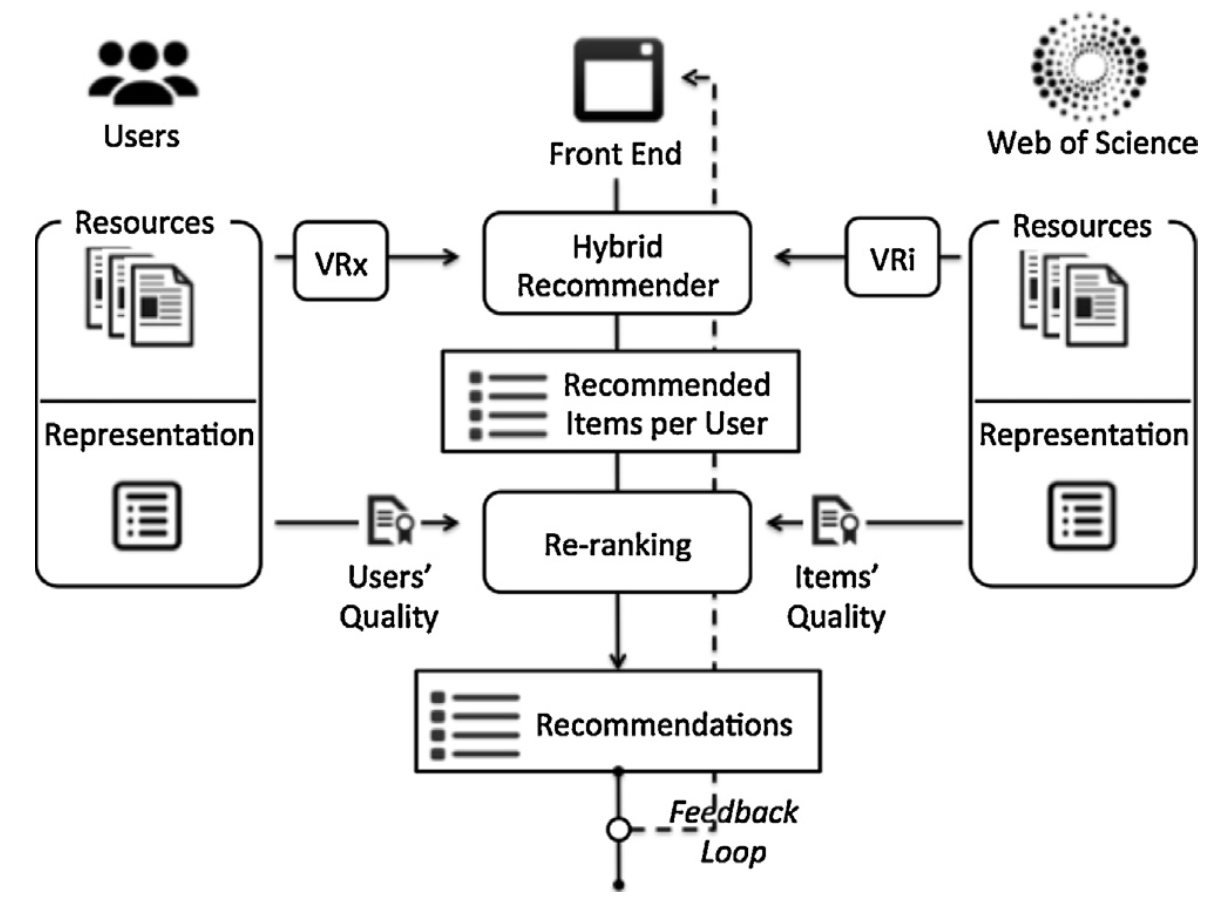
\includegraphics[width=0.6\textwidth]{figures/literature-review/refore.png}
     \rule{35em}{0.5pt}
    \caption{Structure of REFORE system (\textcite{refore})}
 \label{fig:refore}
\end{figure}

In terms of evaluation, the system was tested with a group of researchers from multiple institutions over a year-long period.
Researchers received monthly recommendations based on newly published papers from the Web of Science database, and their feedback was collected to measure the system's effectiveness.
The experimental results demonstrated the system's ability to deliver high-quality and personalized recommendations, outperforming traditional methods by incorporating bibliometric quality measures and user feedback into the hybrid recommendation strategy.

\textcite{Kanwal2024} proposed a research paper recommendation system, integrating citation networks and collaboration networks to provide high-quality and relevant suggestions to researchers.
This approach, named \gls{rrmf}, addresses challenges such as the cold-start problem, data sparsity, and semantic ambiguity.
The proposed methodology involves generating a multi-level citation network, where the focal paper of interest (PI) serves as the central node.
Citation relationships are explored up to six levels, leveraging both forward (citing) and backward (cited by) links.
To evaluate the relevance of papers within the network, bibliographic coupling and co-citation strengths are computed, quantifying the similarity of papers based on shared citations or references.
A candidate score is derived for each paper, which is used to filter irrelevant documents and focus on those most closely related to the paper of interest.
Additionally, centrality measures (such as betweenness, degree, closeness, and eigenvector centrality) are applied to rank papers based on their structural significance within the network.
Papers with high centrality scores are selected for further analysis.
The system extends beyond citation networks by incorporating collaboration networks of authors.
Authors are extracted from top-ranked papers, and their collaboration networks are analyzed using centrality and social measures to identify influential researchers.
These author-based insights contribute to refining paper recommendations, ensuring that suggested papers come from prominent authors within the field.
To evaluate the system, the AMiner dataset, comprising nearly 4.8 million papers and over 45 million citation relationships, was used.
The system's performance was benchmarked using metrics such as \gls{map}, \gls{mrr}, and \gls{ndcg}.
Experimental results demonstrated that the \gls{rrmf} outperformed traditional systems, such as Google Scholar and previous citation-based methods, by achieving higher precision and recall.
The incorporation of multi-level citation analysis and author collaboration measures significantly improved the quality and relevance of recommendations.

\textcite{Murali2019} proposed a research paper recommender system using a user-based \gls{cf} approach.
The goal of the system is to recommend research papers tailored to a user's interests by analyzing their preferences and similarities with other users.
The authors addressed the challenge of information overload faced by researchers due to the rapid growth in the number of research publications.
The system operates by collecting a dataset of user-paper interactions, which includes attributes such as user IDs, paper IDs, and ratings assigned by users to the papers. Based on this data, the system calculates the similarity between users using the cosine similarity measure. This approach evaluates the resemblance between user profiles by treating their preferences as vectors and computing the cosine of the angle between them.
Users with similar interests are identified, and recommendations are generated by predicting ratings for papers based on the ratings given by these similar users.
The block diagram of the system architecture is shown in Fig.~\ref{fig:murali}.
To improve the quality of recommendations, the system utilizes a prediction rating mechanism, which assigns a predicted score to papers based on the \gls{cf} model.
Papers with higher predicted ratings are recommended to the user, ensuring that suggestions align with their preferences.
The authors also implemented a ``user-link formation'' step to construct the \gls{cf} model, leveraging the collective behavior of similar users to refine recommendations further.

\begin{figure}[htbp]
    \centering
 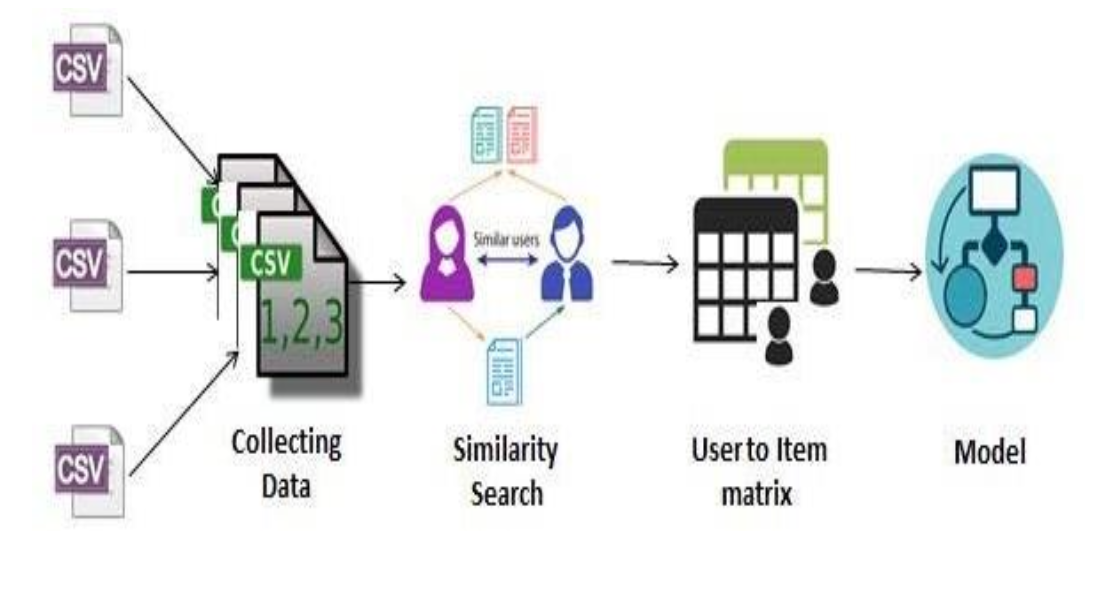
\includegraphics[width=0.65\textwidth]{figures/literature-review/murali.png}
     \rule{35em}{0.5pt}
    \caption{Block diagram of the system architecture (\textcite{Murali2019})}
 \label{fig:murali}
\end{figure}

For evaluation, the system was tested on a dataset comprising 135 users and their interactions with research papers.
Performance was measured using metrics like \gls{mae} and \gls{rmse} to assess the accuracy of predicted ratings against actual ratings.
The results showed that the user-based \gls{cf} model performed well, producing high-quality recommendations with minimal deviation in predicted ratings.
The authors acknowledge limitations in their work, such as the reliance on a synthetic dataset for testing due to the unavailability of real-world datasets with pre-existing paper ratings.
They suggest that the system's effectiveness could be further enhanced if real datasets from platforms like research paper repositories were used.

In their work, \textcite{Sharma2023} present a detailed exploration of research paper recommender systems, addressing their evolution, methodologies, and associated challenges.
It categorizes existing approaches into key methodologies, including \gls{cbf}, \gls{cf}, link-based algorithms, co-occurrence techniques, and hybrid approaches.
Each method is analyzed based on its underlying knowledge sources, such as textual attributes of research papers, author profiles, citation patterns, and user-generated tags, which are leveraged to model user preferences and generate personalized recommendations.
Based on their studies, the authors divide recommender systems into three essential components: the first requirement for performing any task is domain-specific knowledge and its application to the task at hand.
This is called principle or basic knowledge and operational theory.
Principle knowledge includes all available information about an item that is used to perform the recommendation task and serves as key attributes of the system to generate recommendations.
Operational theory, on the other hand, is concerned with the ``how'' aspect, i.e., how the information provided is applied to achieve the intended goals.
The second component is the recommendation approach, which outlines a step-by-step methodology for solving the problem, detailing implementation techniques and their practical implementation.
Finally, the third component, probably the most critical, is user modeling.
The general architecture of a research paper recommendation system is shown in Fig.~\ref{fig:general-architecture-rprs}.

\begin{figure}[htbp]
    \centering
 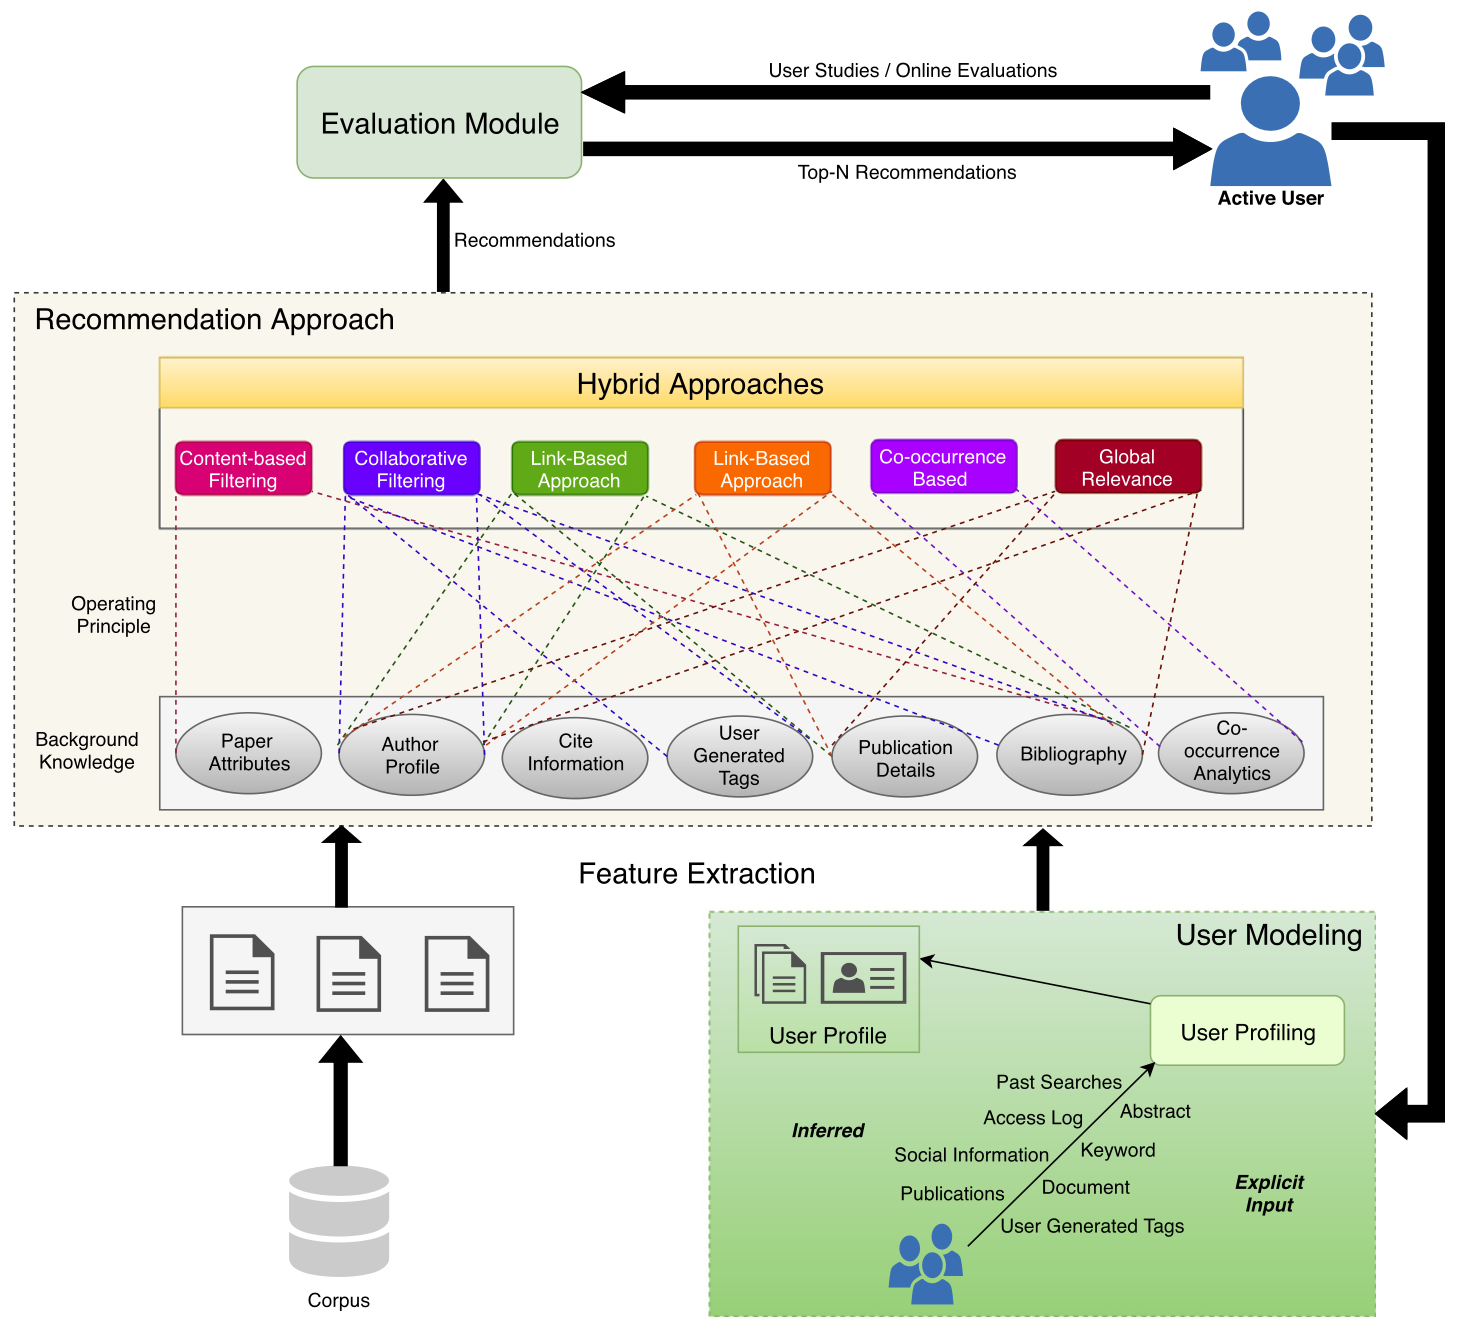
\includegraphics[width=0.7\textwidth]{figures/literature-review/general-architecture-rprs.png}
     \rule{35em}{0.5pt}
    \caption{General architecture of Research Paper Recommendation System (\textcite{Sharma2023})}
 \label{fig:general-architecture-rprs}
\end{figure}

The authors highlight the dominance of \gls{cbf} techniques, which rely on textual similarity between papers and user profiles, and discuss how \gls{cf} leverages peer preferences to improve recommendations.
Hybrid methods, which integrate multiple approaches, are presented as a solution to address the limitations of individual techniques, such as over-specialization in \gls{cbf} and data sparsity in \gls{cf}.
The study also identifies critical challenges, including the lack of standard datasets for benchmarking, insufficient evaluation metrics for dimensions like novelty and serendipity, and the difficulty of scaling algorithms to handle real-world, large-scale datasets.
Furthermore, the paper underscores the need for more sophisticated evaluation frameworks and advanced computational models, such as \gls{dl}, to improve the efficacy and scalability of research paper recommender systems.

\textcite{Jagadishwari2023} proposed a methodology for recommending academic collaborators using a combination of citation analysis and academic influence metrics.
Their work highlights the importance of identifying suitable collaborators to enhance research productivity and addresses the challenges posed by the vast volume of academic data.
The system utilizes the DBLP dataset \cite{Ley2002}, focusing on core computer science publications from 2017 to 2019, and incorporates citation count and influential citation metrics to assess academic influence.
The methodology involves preprocessing the dataset to eliminate irrelevant data, computing an Academic Level Index (ALI) using three different formulae, and then calculating a Research Score (R score) based on ALI and domain-specific publication metrics.
The R score serves as the basis for ranking scholars and identifying potential collaborators.
Three variations of the R score computation are tested, and the study concludes that the third formula (R3 Score) yields the most compatible recommendations by minimizing differences between the scores of the target scholar and recommended collaborators.
The system's results are visualized using graphs and compared across the three scoring methods, demonstrating that R3 Score provides the most precise matches.
The authors suggest future research could include additional factors like geographic location and funding status, as well as expanding the dataset to other academic disciplines.

\textcite{Zhang2023} provide a comprehensive review of scholarly recommendation systems, highlighting their evolution, methodologies, applications, and challenges.
These systems play a crucial role in academia, assisting researchers in identifying relevant literature, potential collaborators, conferences, journals, datasets, and grant opportunities.
The study identifies \gls{cbf} as the most widely used technique, particularly for literature recommendations, whereas \gls{cf} is more prevalent in conference and collaborator recommenders.
Hybrid approaches, which combine \gls{cbf} and \gls{cf}, are also discussed as a promising direction for improving recommendation accuracy and diversity.
The paper evaluates 225 publications across various SRS domains, showing that literature and collaborator recommendation systems dominate the field, while systems for datasets and grants are underexplored.
It notes the limited adoption of deep learning methods in scholarly recommendation systems and emphasizes the need for better integration of user feedback mechanisms to enhance system personalization and effectiveness.
Furthermore, the study highlights the challenges of scalability, data sparsity, and the cold start problem in existing systems.
Evaluation methods, including online and offline metrics, are examined, with offline evaluations being the most common.
In its conclusion, this work stresses the importance of developing unified frameworks that integrate diverse methodologies and leverage advances in \gls{ai} to address current limitations.
It also calls for more research into underrepresented areas like dataset and grant recommendation systems, advocating for user-centric designs that prioritize usability and practical application.

\textcite{Du2022} propose a novel model called ACR-ANE to enhance the recommendation of academic collaborators by integrating network topology and multi-type scholar attributes.
The study addresses the limitations of existing approaches, which often consider only local network structures or singular attribute types, and introduces non-local neighbors to capture stronger academic relationships.
Non-local neighbors are determined through biased random walks and frequency filtering, allowing the model to identify significant connections beyond immediate collaborators.
The methodology incorporates six scholarly attributes-academic age, research interests, publication count, average citations, number of collaborators, and H-index, into a scholar attribute matrix.
These attributes, combined with network structure, are encoded using a deep auto-encoder to generate low-dimensional embeddings that preserve both local and global academic network characteristics.
The model establishes a new multi-type relational network by integrating non-local neighbors and attribute-based proximity, which enriches the representation of academic relationships.
The framework of ACR-ANE is shown in Fig.~\ref{fig:acr-ane}.

\begin{figure}[htbp]
    \centering
 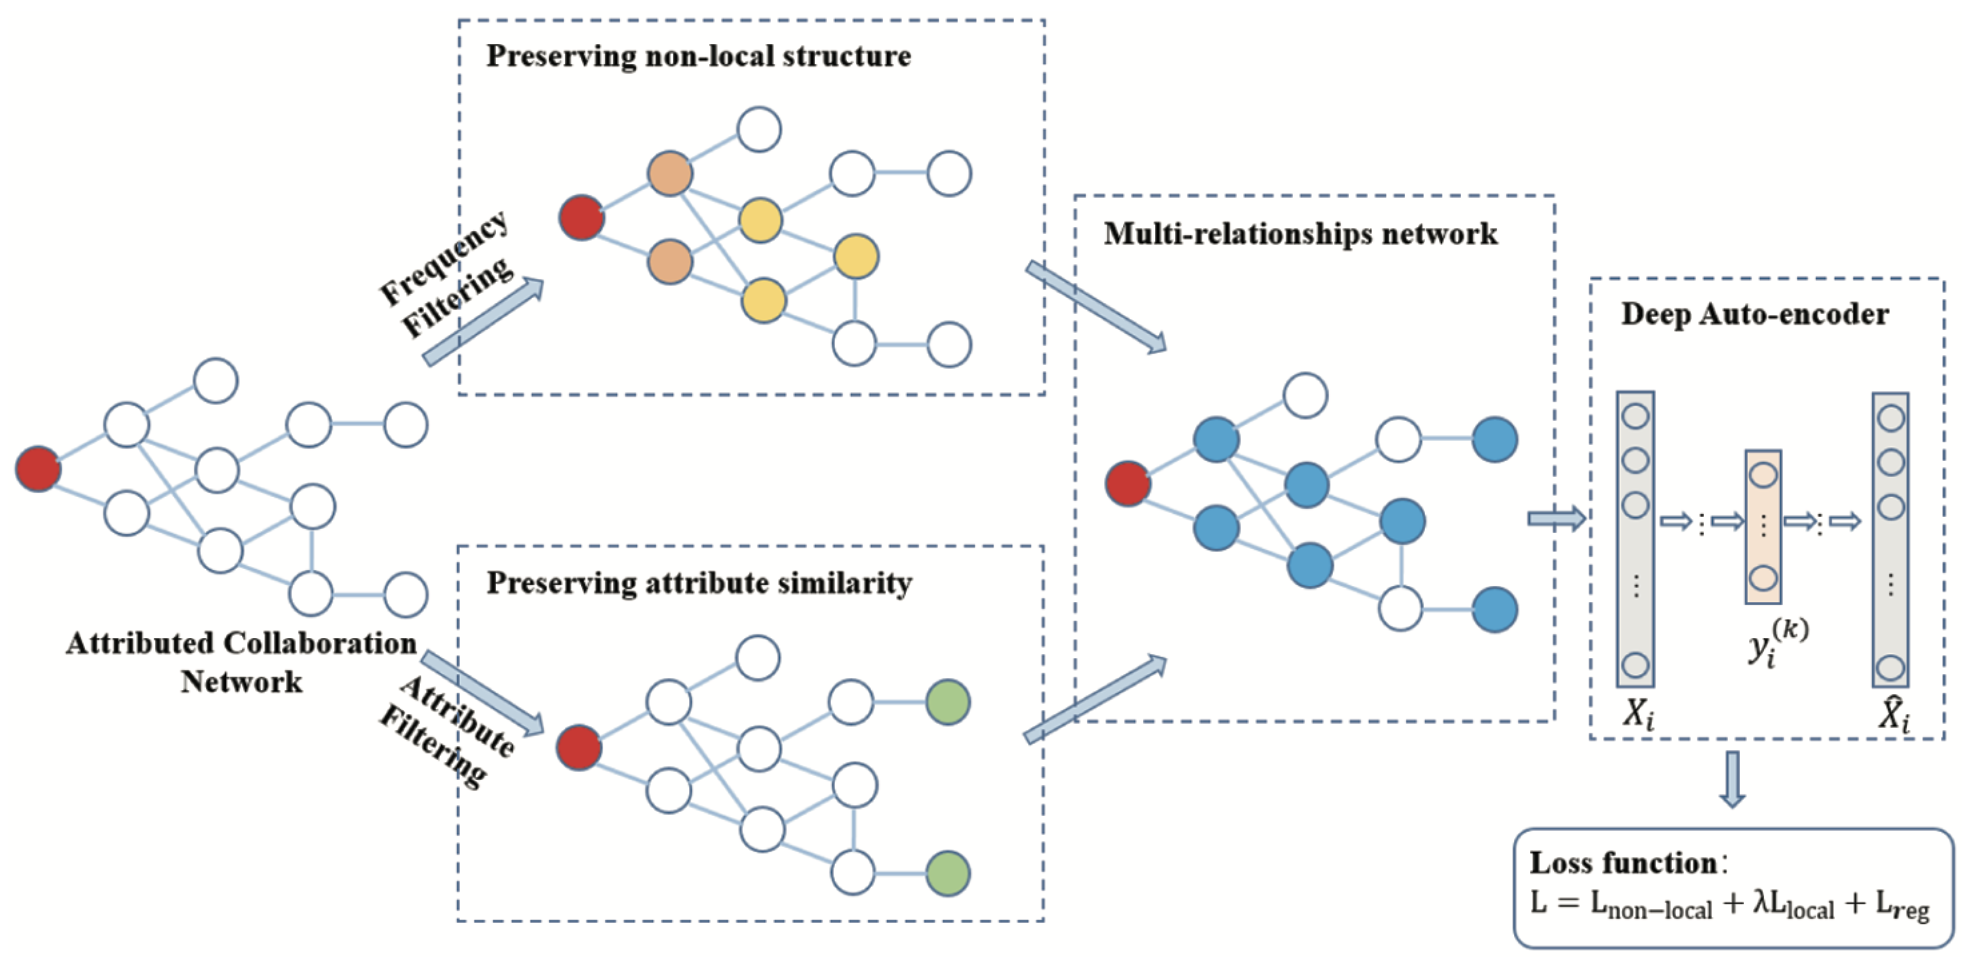
\includegraphics[width=0.8\textwidth]{figures/literature-review/academic-collaborator-recommendation-framework.png}
     \rule{35em}{0.5pt}
    \caption{The framework of ACR-ANE model. (\textcite{Du2022})}
 \label{fig:acr-ane}
\end{figure}

Extensive experiments conducted on two real-world datasets, Aminer and APS, demonstrate the superior performance of ACR-ANE in comparison to baseline models such as DeepWalk, TADW, SDNE, and ACNE.
The results highlight the effectiveness of combining network structure and scholar attributes for collaborator recommendation.
However, the study acknowledges its limitation in handling dynamic networks and suggests future work on incorporating temporal factors to reflect evolving academic collaborations.

\textcite{Zhu2022} explore the application of \glspl{gnn} to recommend research collaborators in the academic domain.
The study focuses on leveraging dynamic and temporal aspects of research networks, addressing the challenge of identifying suitable collaborators in a rapidly evolving academic landscape.
The authors utilize data from the MEDLINE database and implement two \gls{gnn}-based models, GraphSAGE and \gls{tgn}, to capture both static and temporal dependencies among researchers.
GraphSAGE employs an inductive approach that generates embeddings for unseen nodes by aggregating neighbor features, making it suitable for large and dynamic graphs.
\gls{tgn} extends this by incorporating temporal elements, using a message-passing mechanism to update node embeddings based on time-stamped interactions.
These models are compared against baseline methods, including the transductive LightGCN and a \gls{gbc}.
The study is divided into two experimental scenarios: automatic evaluations using \gls{auc} and average precision metrics, and external evaluations based on user ratings collected via a web-based application.
Results indicate that \gls{tgn} outperforms other methods in handling temporal dynamics and inductive tasks, particularly when using publication titles as node features.
While GraphSAGE exhibits strong performance for static embeddings, \gls{tgn} demonstrates superior capability in predicting future collaborations by integrating time-sensitive relationships.
The authors acknowledge limitations such as the small sample size in external evaluations and the reliance on static node features for some tests.
They propose future enhancements, including the integration of distribution-based representations for nodes to better manage uncertainty and improve predictive modeling.

\subsection*{Retrieval-Augmented Recommender Systems}\label{sec:retrieval-augmented-recommender-systems-in-research-field}

As described in Sec.~\ref{sec:retrieval-augmented-generation} and according to \textcite{Deldjoo2024}, \gls{rag} leverages the integration of retrieval systems and generative models to produce highly relevant and context-aware recommendations.
This approach stores knowledge externally, allowing dynamic updates and reducing the risk of hallucinations by grounding outputs in retrieved data.
By minimizing the need for extensive model parameters, \gls{rag} improves efficiency and makes complex tasks, such as generating personalized explanations, more feasible.
However, its effectiveness is strictly linked to the quality and relevance of the retrieved information, making it reliant on robust retrieval systems and well-curated external knowledge bases.
Additionally, the integration of retrieval and generation components introduces complexity and potential computational overhead, especially in real-time applications.
Despite these challenges, \gls{rag} offers a powerful framework for enhancing the accuracy and adaptability of modern recommender systems.

For example, \textcite{Banerjee2024} propose an approach to improve tourism recommender systems by integrating sustainability considerations into the recommendation process.
The authors leverage \gls{rag} to enhance \glspl{llm} for generating recommendations, focusing on sustainable city trips in Europe.
Their main innovation is the incorporation of a sustainability metric during the \gls{rag} pipeline's prompt augmentation phase, called Sustainability Augmented Reranking (SAR).
Fig.~\ref{fig:sar-enhanced-recommendation} illustrates the SAR-enhanced recommendation process, which adjusts the traditional \gls{rag} pipeline by including a sustainability metric based on city popularity and seasonal demand.

\begin{figure}[htbp]
    \centering
    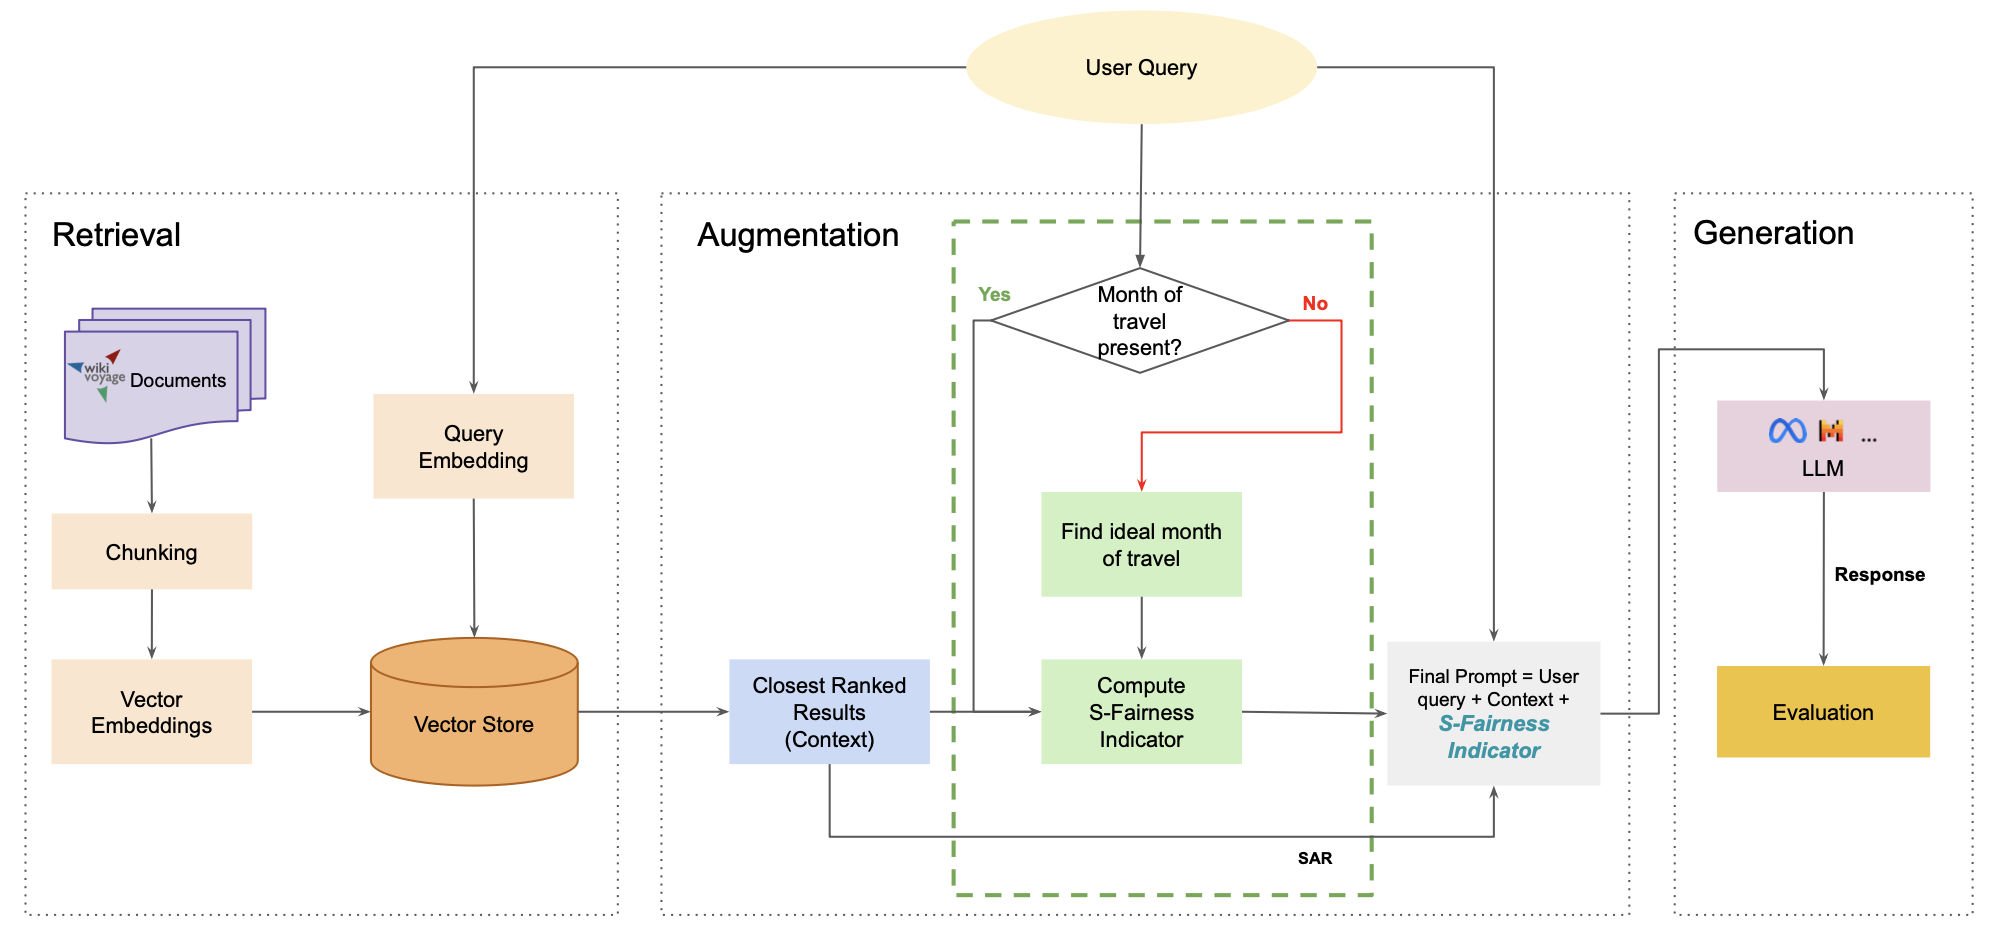
\includegraphics[width=0.8\textwidth]{figures/literature-review/rag-tourism.png}
    \rule{35em}{0.5pt}
    \caption{SAR-enhanced recommendation process (\textcite{Banerjee2024})}
 \label{fig:sar-enhanced-recommendation}
\end{figure}

The SAR enhancement adjusts the traditional \gls{rag} process by including a sustainability metric based on city popularity and seasonal demand.
This metric helps the system prioritize recommendations that align with sustainability principles, such as promoting destinations with lower tourism pressure during certain months.
By leveraging data from sources like Wikivoyage\footnote{\url{https://www.wikivoyage.org}} and Tripadvisor\footnote{\url{https://www.tripadvisor.com}}, the system calculates popularity and seasonality indices to inform the SAR metric, ensuring that recommendations balance user preferences with environmental and societal considerations.
Using open-source \glspl{llm}, such as Llama-3.1-Instruct-8B and Mistral-Instruct-7B, the study demonstrates that SAR-enhanced recommendations perform equal to or better than baseline models (without SAR) in terms of quality and sustainability.
The approach reduces common issues in \gls{llm}-based TRS, like hallucinations, and supports a multi-stakeholder perspective by addressing the needs of users, local communities, and environmental sustainability.

Another example is \gls{ramo}, a system designed to enhance Massive Open Online Courses (MOOCs) recommendations by addressing the ``cold start'' problem common in recommender systems \cite{Rao2024}.
Traditional course recommendation systems often struggle with new users due to the absence of historical data.
\gls{ramo} tackles this limitation by leveraging a \gls{rag} pipeline integrated with \gls{llm}.
In \gls{ramo}, the \gls{rag} framework combines two key components: a retriever and a generator.
The retriever accesses a pre-built knowledge base of course data, such as Coursera's publicly available dataset, and retrieves relevant information based on user queries.
The retrieved content is used to augment the prompts provided to the generator, ensuring responses are contextually relevant and precise.
This setup enables \gls{ramo} to generate personalized course recommendations even when little or no user-specific information is available, thereby overcoming the cold start issue.
The \gls{ramo} system workflow is shown in Fig.~\ref{fig:ramo-system-workflow}.

\begin{figure}[htbp]
    \centering
    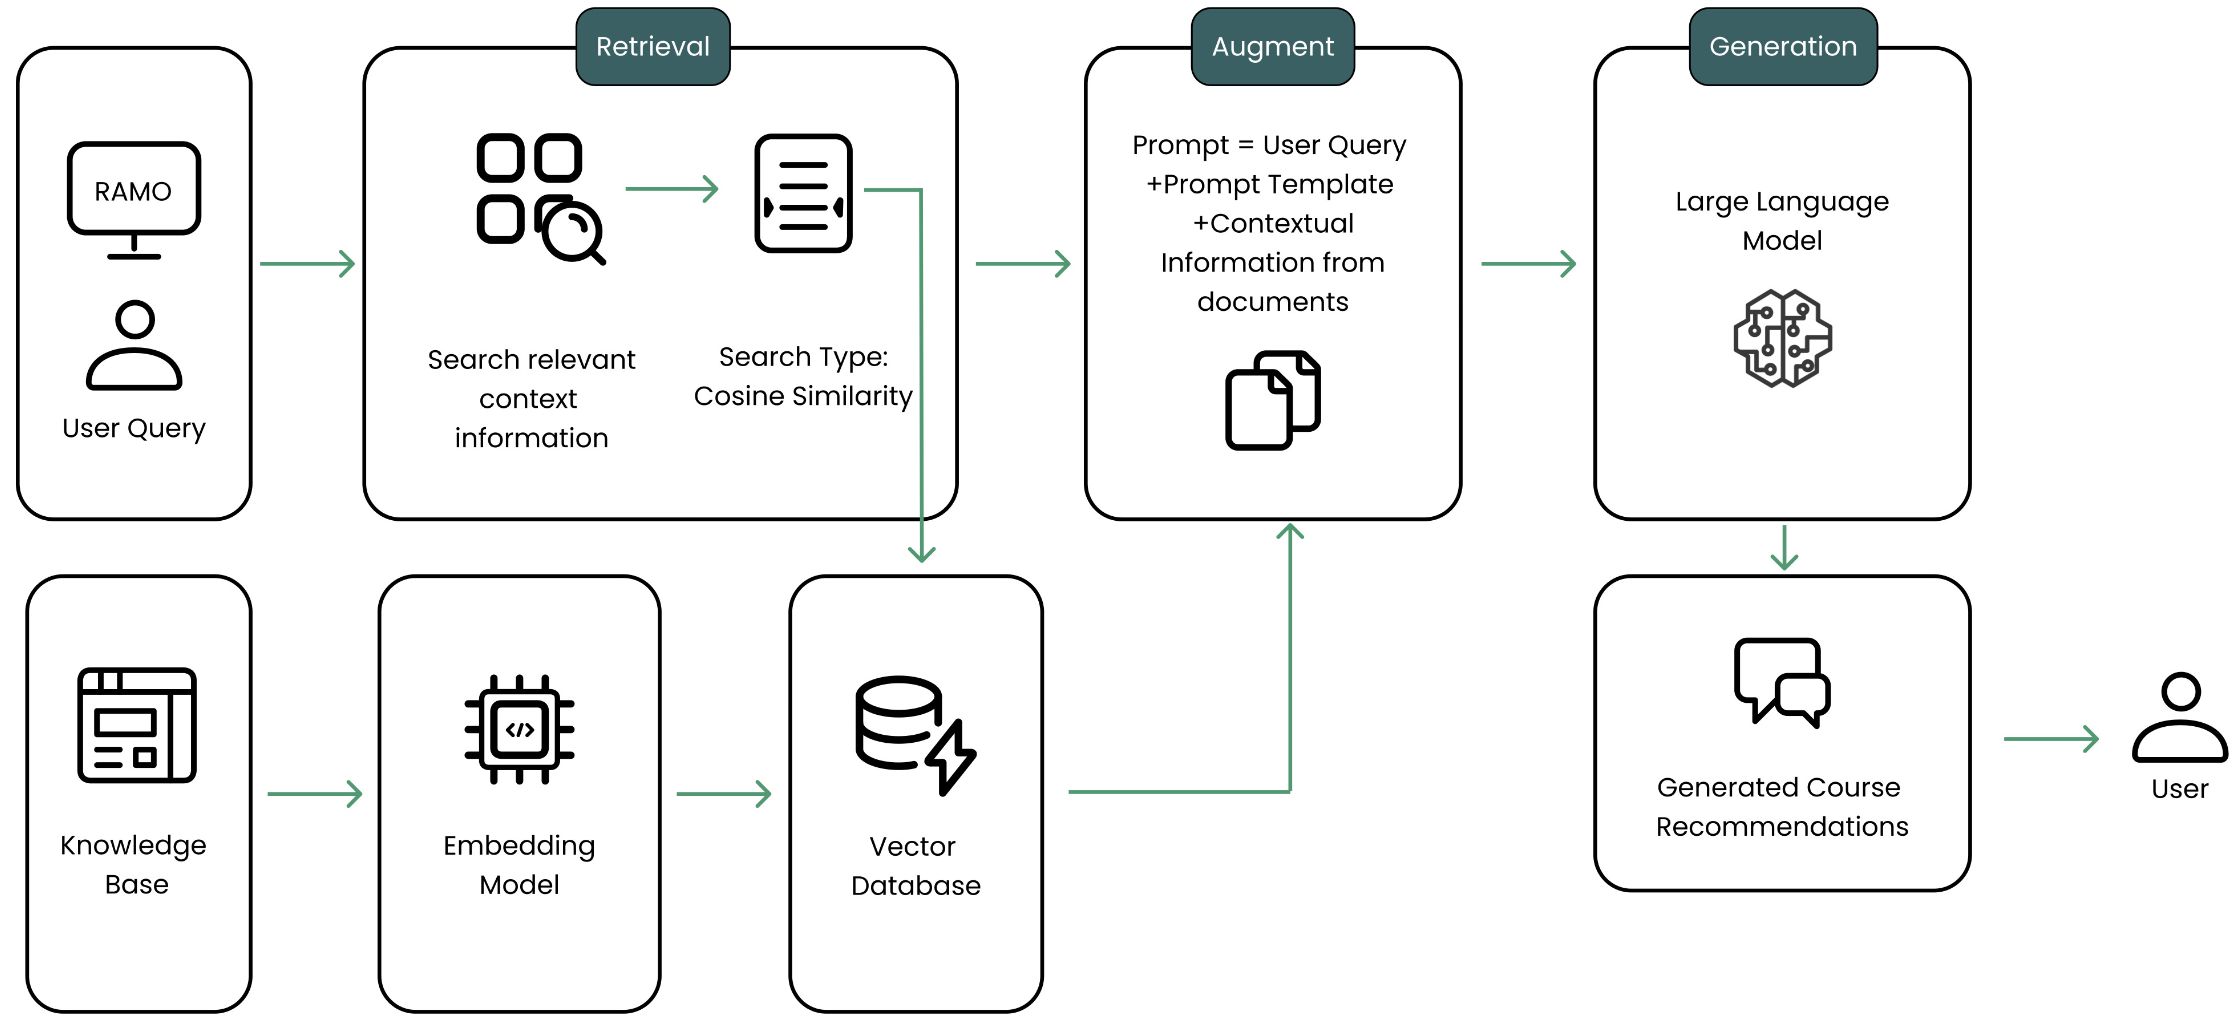
\includegraphics[width=0.8\textwidth]{figures/literature-review/ramo.png}
    \rule{35em}{0.5pt}
    \caption{The \gls{ramo} System workflow (\textcite{Rao2024})}
 \label{fig:ramo-system-workflow}
\end{figure}

The system utilizes advanced text embedding techniques to store and retrieve course data efficiently, employing models like OpenAI's text-embedding-ada-002 for embedding generation.
The final recommendations are produced by GPT-3.5 Turbo, selected for its cost-efficiency and performance, allowing dynamic, conversational interaction with users.
The paper evaluates \gls{ramo} by comparing its performance to traditional systems and standard \gls{llm}-based recommenders without \gls{rag}.
Results show that the \gls{rag}-enhanced system delivers more personalized and flexible recommendations, particularly in scenarios requiring personalized suggestions or dealing with general queries from new users.
The integration of \gls{rag} also ensures that the recommendations align closely with user needs by dynamically retrieving and incorporating domain-specific knowledge.

\textcite{DiPalma2023} explore the integration of \glspl{llm} into recommender systems to address challenges like cold-start problems, data sparsity, and adaptability to unseen data.
While traditional methods such as \gls{cf}, matrix factorization, and \gls{cbf} are effective in structured domains, they struggle in dynamic environments.
In contrast, \glspl{llm} leverage vast pre-trained knowledge, enabling them to generate meaningful recommendations even in novel scenarios.
To combine these strengths, the paper proposes a Retrieval-Augmented Recommender System that integrates retrieval-based and generative models to enhance accuracy and explainability.
This framework allows recommender systems to retrieve relevant external knowledge while using \glspl{llm} for improved reasoning and contextual adaptation.
The study examines \glspl{llm} in two roles: at the higher level, powering conversational \gls{ai} for personalized recommendations, and at the lower level, refining recommendation strategies through knowledge retrieval and generation.
Evaluating GPT-3.5 on MovieLens100K and Facebook Books datasets, the study compares its performance with state-of-the-art baselines using accuracy metrics such as nDCG, HR, and MAP.
GPT-3.5 performs competitively, particularly excelling in book recommendations due to its extensive pretraining on book-related data.
In movie recommendations, its performance is slightly lower than top models, highlighting the need for fine-tuning or retrieval augmentation.
Despite its potential, several challenges arise in integrating \glspl{llm} into recommender systems.
The cold-start problem persists, as effectiveness varies by dataset and domain.
Hallucination remains an issue, with models generating inaccurate or non-existent recommendations.
Popularity bias limits diversity, and the lack of real-time updates prevents awareness of newly introduced items.
Additionally, the black-box nature of \glspl{llm} raises concerns about explainability compared to traditional, more interpretable recommender systems.

\textcite{Wu2024} addresses the challenge of long-tail recommendation, where traditional \gls{cf}-based recommender systems struggle due to data sparsity and imbalance.
While \glspl{llm} have demonstrated strong reasoning capabilities, they typically rely on item semantics and fail to capture collaborative user-item interaction patterns, leading to misaligned recommendations.
To overcome this limitation, the authors introduce CoRAL, a collaborative retrieval-augmented \gls{llm} framework that integrates collaborative evidence into \gls{llm} prompts, ensuring alignment with real-world user-item interactions.
CoRAL enhances recommendation performance by retrieving minimal-sufficient collaborative information through a reinforcement learning-based retrieval policy, optimizing the inclusion of relevant interactions while minimizing unnecessary data that could distract the \gls{llm}.
The framework formulates long-tail recommendation as a sequential decision-making problem, where the retrieval policy dynamically selects user-item interactions to support the \gls{llm}'s reasoning process.
Experimental evaluations on Amazon product datasets demonstrate that CoRAL significantly outperforms both traditional \gls{cf} methods and standard \gls{llm}-based recommendation approaches, achieving superior accuracy in predicting user preferences.
The study highlights the importance of integrating collaborative knowledge with \glspl{llm} for long-tail recommendation and suggests reinforcement learning as a viable approach for optimizing retrieval-augmented recommendations.
%
\section{Literature Requirements}\label{sec:literature-requirements}
The following \glspl{lr} were selected from the relevant works in the literature.
Several \glspl{kg} exist in the research and scholarly fields, but no work uses them in the European research domain.
The definition of an ontology and/or use of a \gls{kg} in this domain is necessary in order to allow semantic representation of European projects (\gls{lr}1).
Among current research recommender systems, some exploit various filtering approaches including \gls{cbf}.
Generating \gls{cbf} recommendation could be quite efficient (\gls{lr}2), for example if based on a project description or abstract, recommend potential collaborators, who have collaborated on a project with that description similar to the one specified.
Unfortunately, some \gls{dl}-based recommender systems need data training to perform the assigned task.
In some cases it may also be necessary to retrain the model.
In these cases, generating recommendations without performing either training or other techniques such as fine-tuning helps to save computational power (\gls{lr}3).
Regarding the hop reasoning perspective, retrieving relevant information dynamically, using models such as \glspl{gnn}, can require high computations on graphs, especially on large graphs (\gls{lr}4).
Table~\ref{tab:literature-requirements} shows the list of \glspl{lr} and their corresponding description.

\begin{table}[htbp]
    \centering
    \scriptsize
    \begin{tabularx}{\textwidth}{|>{\centering\arraybackslash}p{2cm}|X|}
      \hline
      \textbf{Literature Requirement} & \textbf{Description}\\
        \hline
        \gls{lr}1 & Definition of an ontology and/or use of a \gls{kg} in the European research domain \\
        \gls{lr}2 & Exploitation of \gls{cbf} in research recommender systems \\
        \gls{lr}3 & Generation of recommendations without training or fine-tuning \\
        \gls{lr}4 & High computational power for dynamic retrieval of relevant information using \glspl{gnn} \\
        \hline
    \end{tabularx}
    \caption{List of \acrfullpl{lr} and their corresponding description}
    \label{tab:literature-requirements}
\end{table}

\fillingPage{}
\chapter{Research Design}\label{chap:research-design}

The research design is the general plan for conducting a study, ensuring that the research questions are addressed effectively.
According to \textcite{SaundersMark2023}, the research design outlines the overall strategy that integrates the different components of the study in a coherent and logical manner, thus ensuring that the study effectively addresses the research question.
Fig.~\ref{fig:research-onion} illustrates the research onion, which provides a structured approach to the conceptualisation of research design by stripping away various layers, including research philosophy, research approach, methodological choice, strategy, time horizon, and data collection techniques and procedures.
This chapter will briefly discuss each of these layers, providing a comprehensive overview of the chosen research design for this study.

\begin{figure}[htbp]
    \centering
 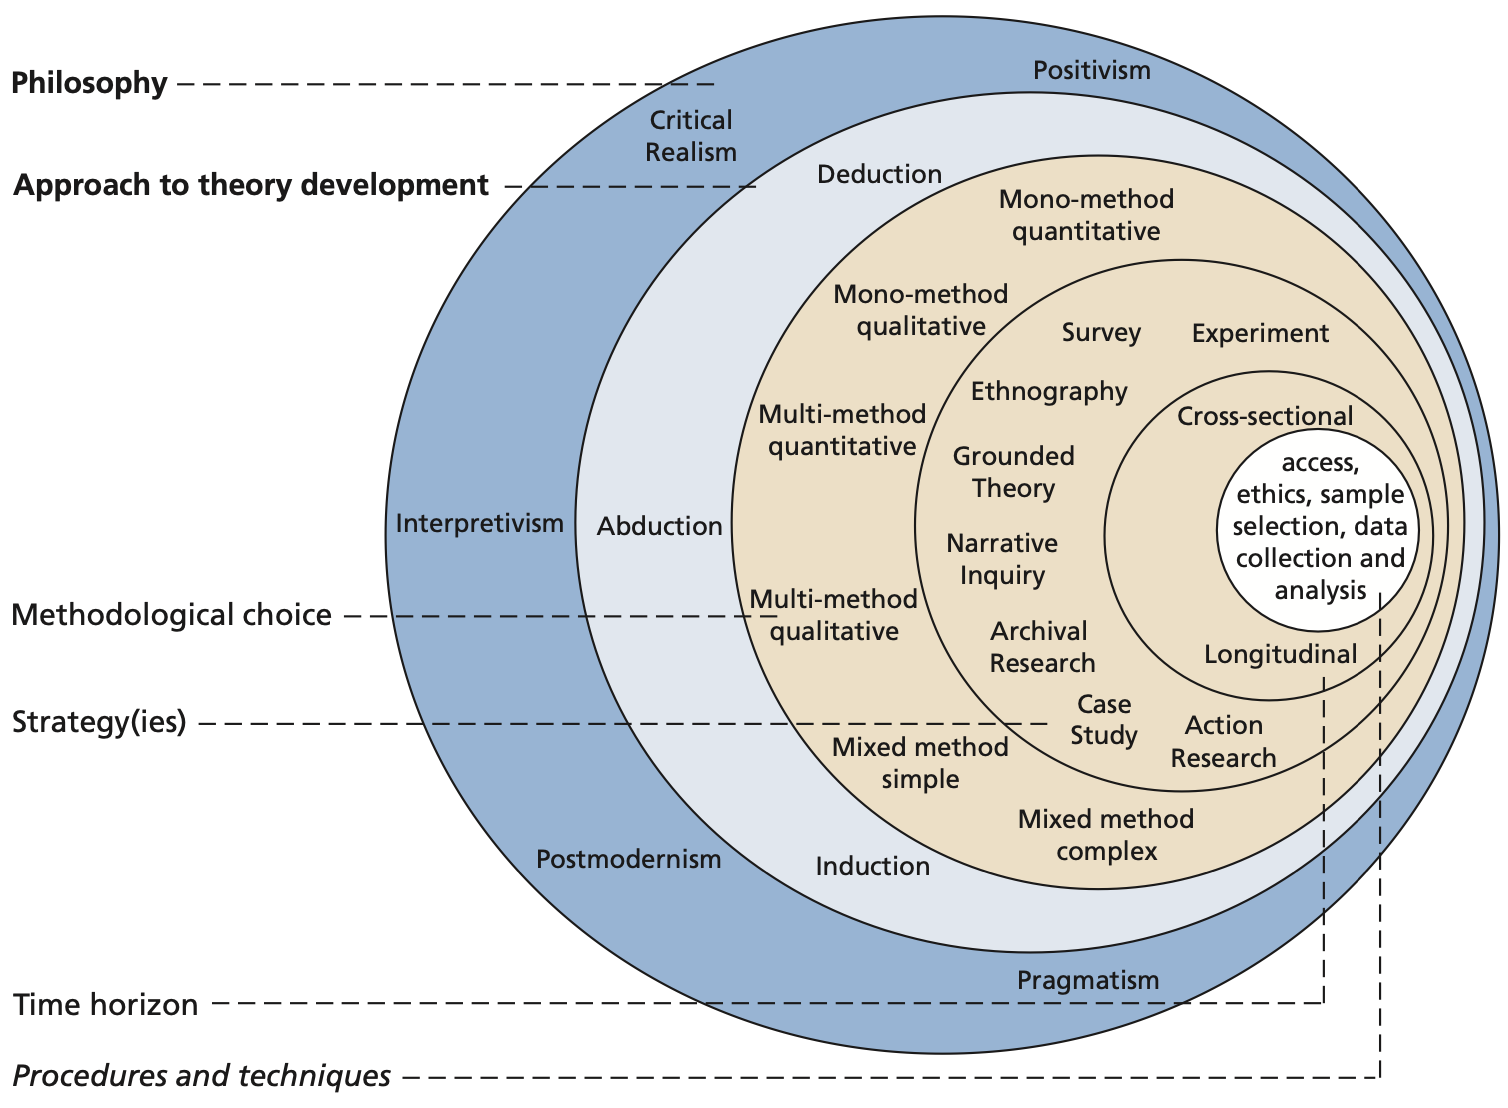
\includegraphics[width=.9\textwidth]{figures/research-design/research-onion.png}
     \rule{35em}{0.5pt}
    \caption{The Research onion (\textcite{SaundersMark2023})} 
 \label{fig:research-onion}
\end{figure}

\section{Research Philosophy}\label{sec:research-philosophy}
Research philosophy is the first layer of the research onion and refers to the set of beliefs and assumptions that establish the research process.
Following the research onion \cite{SaundersMark2023}, the main philosophies that a researcher can adopt are positivism, critical realism, interpretivism, postmodernism, and pragmatism.

\textit{Positivism} is based on the idea of working with an observable social reality and that the end product of such research can be generalisations similar to those produced by physical and natural scientists.
Since it argues for an objective reality that can be measured by quantitative methods, this thesis does not follow this approach as the main objective is not to generalise the findings.
\textit{Critical realism} is based on the idea that the social world is not a direct reflection of the physical world, but that it is constructed by individuals based on their experiences and perceptions.
This approach is also not followed in this study as it is more focused on understanding the social world as it is perceived by the participants.
\textit{Interpretivism} emphasizes the importance of understanding the differences among human beings in their roles as social actors.
It highlights the distinction between conducting research involving people, who interpret and assign meaning to their experiences, as opposed to research involving inanimate objects.
This thesis does not follow this philosophy because it does not explore subjective human experiences and social constructs.
\textit{Postmodernism} challenges established ideas by emphasizing the role of language, power, and cultural context in shaping reality.
It rejects the notion of a single objective truth, arguing instead for multiple, evolving perspectives influenced by social constructs.
This philosophy is not followed in this thesis as it does not aim to challenge established ideas or explore the role of language, power, and cultural context in shaping reality.
Finally, \textit{pragmatism} focuses on practical solutions, asserting that research should be guided by the problem at hand rather than rigid philosophical stances.
It promotes flexibility by combining qualitative and quantitative methods to achieve useful and actionable outcomes.

This thesis follows a pragmatic approach in that it aims to address the problem of finding collaborators for a given research project.
%
\section{Research Approach}\label{sec:research-approach}
According to \textcite{SaundersMark2023}, the second layer of the research onion is the research approach, which is the strategy that the researcher can use to start the research.
There are three main research approaches.
\textit{Deductive} approach, that begins with established theories or hypotheses and tests them through empirical data collection, following a structured and logical progression to confirm or refute existing concepts.
In contrast, \textit{inductive} approach involves deriving theories from observed data, allowing patterns and relationships to emerge without predefined expectations.
\textit{Abductive} approach combines elements of both, iteratively moving between theory and data to refine explanations and generate new insights based on surprising observations.

This thesis follows the inductive approach because the aim is to design and develop a system that is based on a data domain, the European research domain.
The data collection to provide this recommendation of collaborators starts with the research questions for analysis, experiments and evaluation of a prototype.
This prototype will be based on a hybrid \gls{ai} approach, the performance of which will be measured by certain evaluation metrics.
The results obtained will be used to prove the thesis statement.
%
\section{Methodological Choice}\label{sec:methodological-choice}
The third layer of the research onion is the methodological choice, which refers to the specific techniques and procedures used to collect and analyze data.
According to \textcite{SaundersMark2023}, the methodological choice is influenced by the research philosophy and approach.

Research can be conducted using either a quantitative or qualitative approach, depending on the objectives pursued.
Quantitative research is primarily concerned with hypothesis testing through a deductive approach or pattern discovery when adopting an inductive perspective.
In both cases, the analysis relies on a large volume of data to ensure statistical significance.
In contrast, qualitative research focuses on smaller datasets, aiming to capture the underlying characteristics within them.

This thesis use a qualitative research approach, as the primary goal is to understand the research domain and the challenges faced by researchers in finding collaborators.
%
\section{Research Strategy}\label{sec:research-strategy}
The research strategy defines how the research goal is to be achieved \cite{SaundersMark2023}.
This aspect of the research design is crucial as it outlines the steps to be taken to address the research questions effectively.
Several research strategies have been defined including: Experiment, Survey, Case study, Action research, Grounded theory, Ethnography and Archival research.
Each of these strategies is designed with a specific purpose in mind and is best suited to achieving the intended research objective.

Since the primary goal of this thesis is to design and develop an artefact, the research strategy used is the \gls{dsr} \cite{Hevner2010}.
\gls{dsr} is a research methodology that focuses on what is called ``relevance'', which is the creation and evaluation of an artifact to solve complex real-world problems.
Moreover, the research should enhance the existing body of knowledge, a principle referred to as ``rigor''.
This duality emerges from the fundamental idea that \gls{dsr} combines two distinct research paradigms: behavioral science and design science, each serving unique objectives to achieve the overall research goals.
A proposed Information Systems Research framework (Fig.~\ref{fig:information-system-research-framework}) illustrates this dual nature, emphasizing the necessity of addressing both a practical business need and the application of relevant knowledge in the research process.

\begin{figure}[htbp]
    \centering
 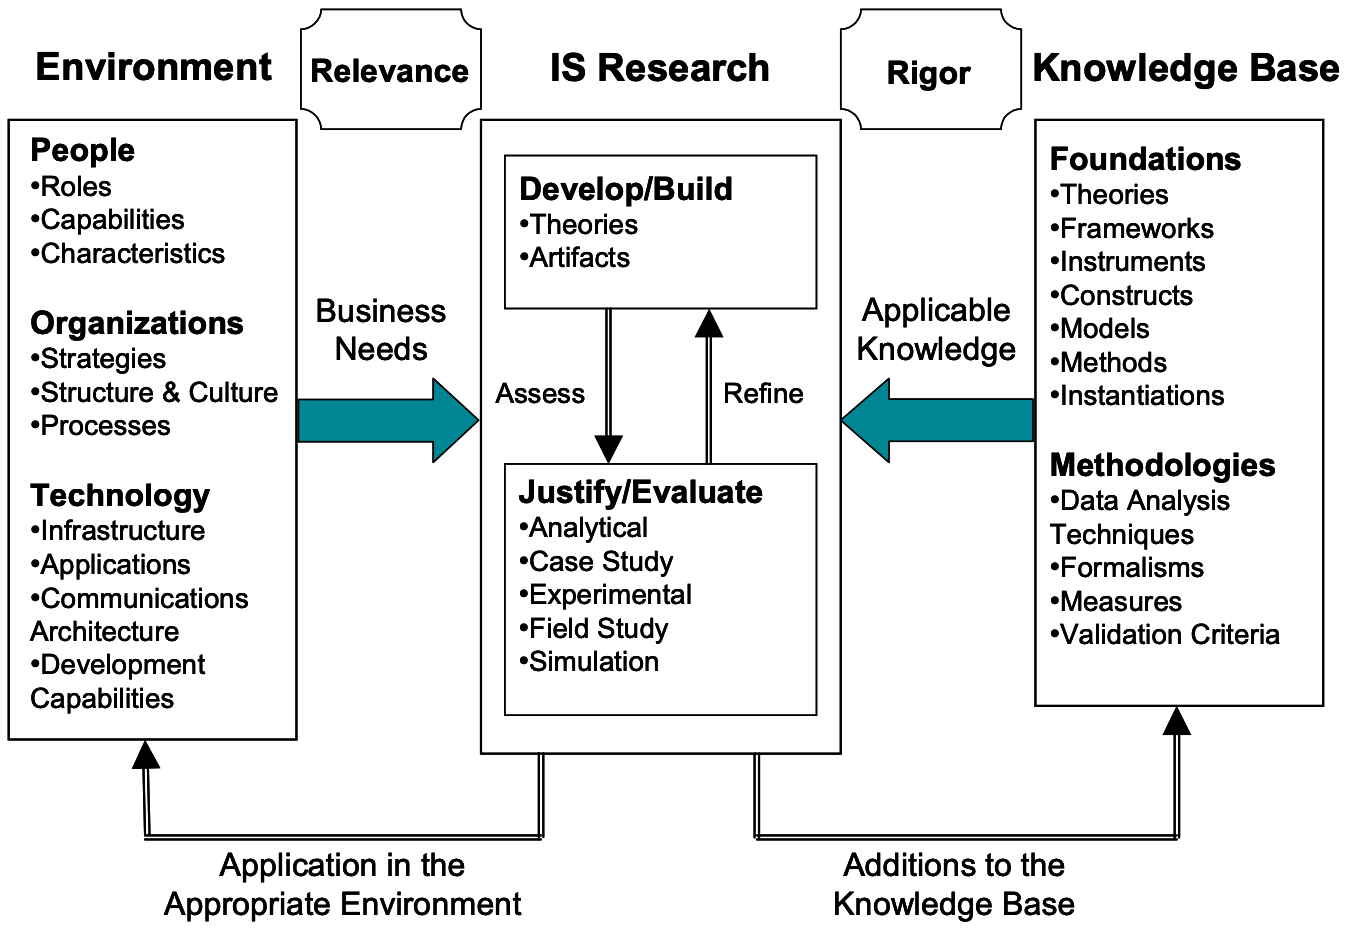
\includegraphics[width=.9\textwidth]{figures/research-design/information-system-research-framework.png}
     \rule{35em}{0.5pt}
    \caption{Information Systems Research Framework (\textcite{Hevner2010})} 
 \label{fig:information-system-research-framework}
\end{figure}

As already mentioned, the \gls{dsr} focuses on the creation and evaluation of an artifact to solve complex real-world problems.
The \gls{dsr} process is iterative, involving multiple cycles of development and evaluation, as illustrated in Fig.~\ref{fig:design-science-research-cycles}.

\begin{figure}[htbp]
    \centering
 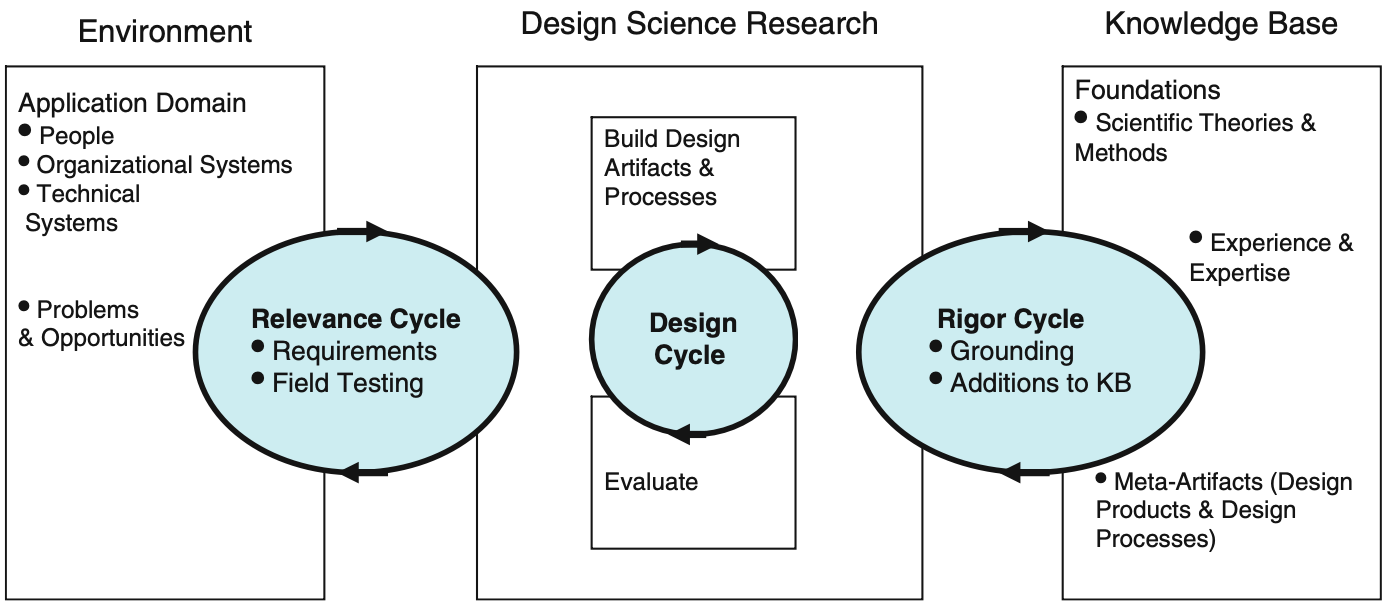
\includegraphics[width=.9\textwidth]{figures/research-design/design-science-research-cycles.png}
     \rule{35em}{0.5pt}
    \caption{\acrlong{dsr} Cycles (\textcite{Hevner2010}) } 
 \label{fig:design-science-research-cycles}
\end{figure}

On the right side, the Rigor Cycle focuses on existing knowledge, incorporating theories, methodologies, and expert experiences.
In the context of this thesis, it represents the literature review.
On the left side, the Relevance Cycle highlights the application domain, encompassing the people, organizations, systems, and the challenges or opportunities they face.
At the center, there is the Design Cycle, which addresses research through the development and evaluation of the artifact.
These three components are interconnected, forming a continuous \gls{dsr} cycle that ensures the integration of knowledge, practical relevance, and iterative refinement.

According to \textcite{Hevner2010}, the \gls{dsr} is defined in five process steps: awareness of problem, suggestion, development, evaluation, and conclusion.
\textcite{Hevner2010} modified a framework originally proposed by \textcite{Vaishnavi2007}, illustrating the five process steps along with the expected outputs and knowledge flows, as illustrated in Fig.~\ref{fig:design-science-research-framework}.

\begin{figure}[htbp]
    \centering
 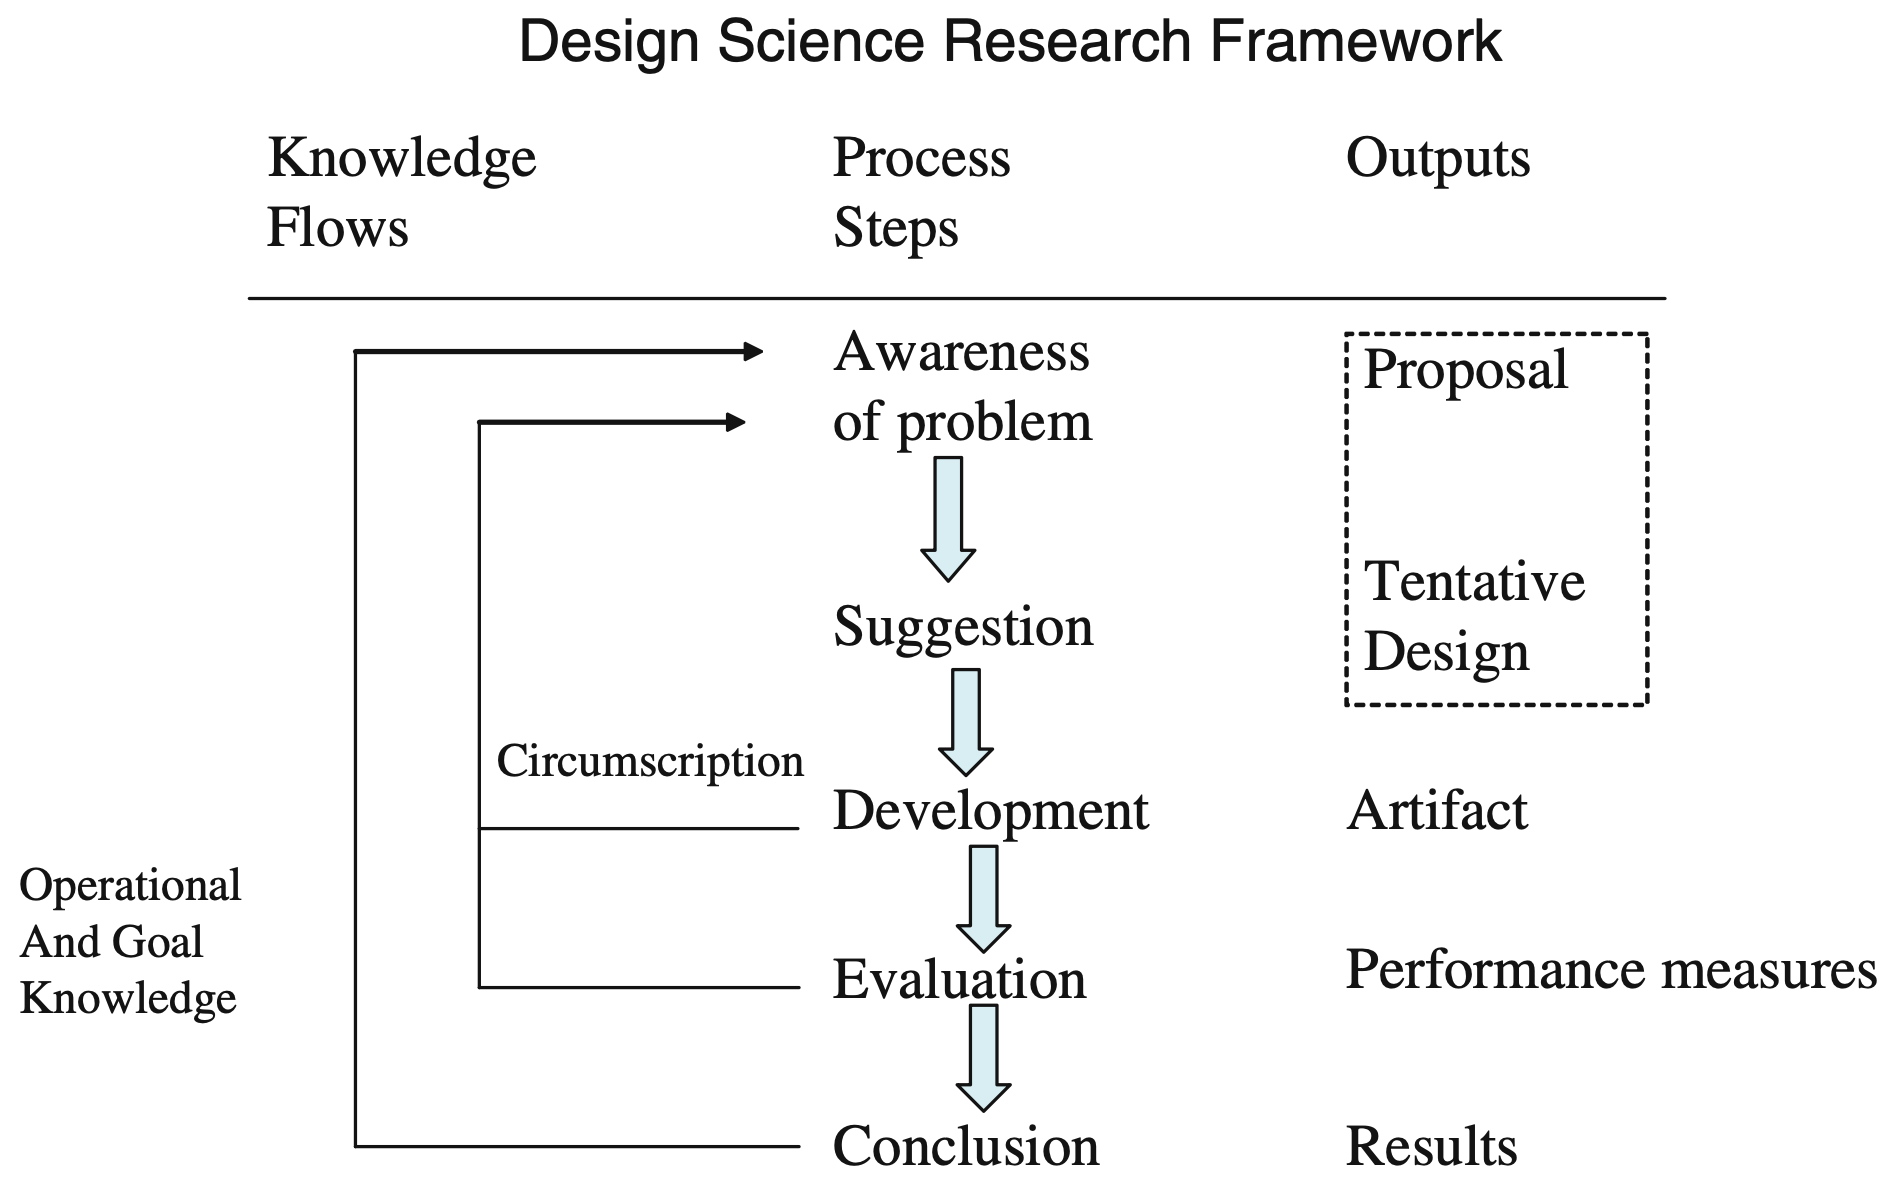
\includegraphics[width=.9\textwidth]{figures/research-design/design-science-research-framework.png}
     \rule{35em}{0.5pt}
    \caption{\acrlong{dsr} Framework (\textcite{Hevner2010}) adapted from (\textcite{Vaishnavi2007})} 
 \label{fig:design-science-research-framework}
\end{figure}

The research of this thesis will follow the \gls{dsr} methodology, in accordance with the five steps of the framework proposed by \textcite{Hevner2010}.

The Awareness Phase involves researchers identifying and recognizing a specific problem or opportunity that requires attention.
During this initial stage, they gain a clear understanding of existing challenges or gaps in current systems or processes, laying the groundwork for the subsequent phases of the design cycle.

In the Suggestion Phase, researchers propose potential solutions to address the identified problem or opportunity.
This stage focuses on generating innovative ideas and design concepts that serve as the foundation for developing artifacts aimed at resolving the issue.

The Development Phase is where researchers build and implement the designed artifacts or solutions based on the proposals from previous phases.
This stage transforms conceptual designs into functional prototypes, bringing the ideas to life.

During the Evaluation Phase of \gls{dsr}, researchers analyze and assess the developed artifacts to determine their effectiveness and performance.
This stage involves rigorous testing, validation, and evaluation of the solutions against predefined criteria and objectives.
Stakeholder feedback may also be collected to refine and enhance the artifacts further.
The primary goal of this phase is to ensure that the designed solutions effectively address the identified problem and meet the intended requirements.

Finally, the Conclusion Phase involves drawing insights and summarizing findings based on the outcomes of the evaluation phase.
Researchers reflect on the effectiveness of the designed artifacts, assess their impact on solving the identified problem, and evaluate their overall contribution to the research objectives.

Fig.~\ref{fig:design-science-research-framework-adapted-by-author} illustrates the \gls{dsr} framework adapted by the author, which will be used to guide the research process in this thesis.
Each of these \gls{dsr} steps applied to this thesis is mapped and described in the following chapters.
\begin{figure}[htbp]
    \centering
 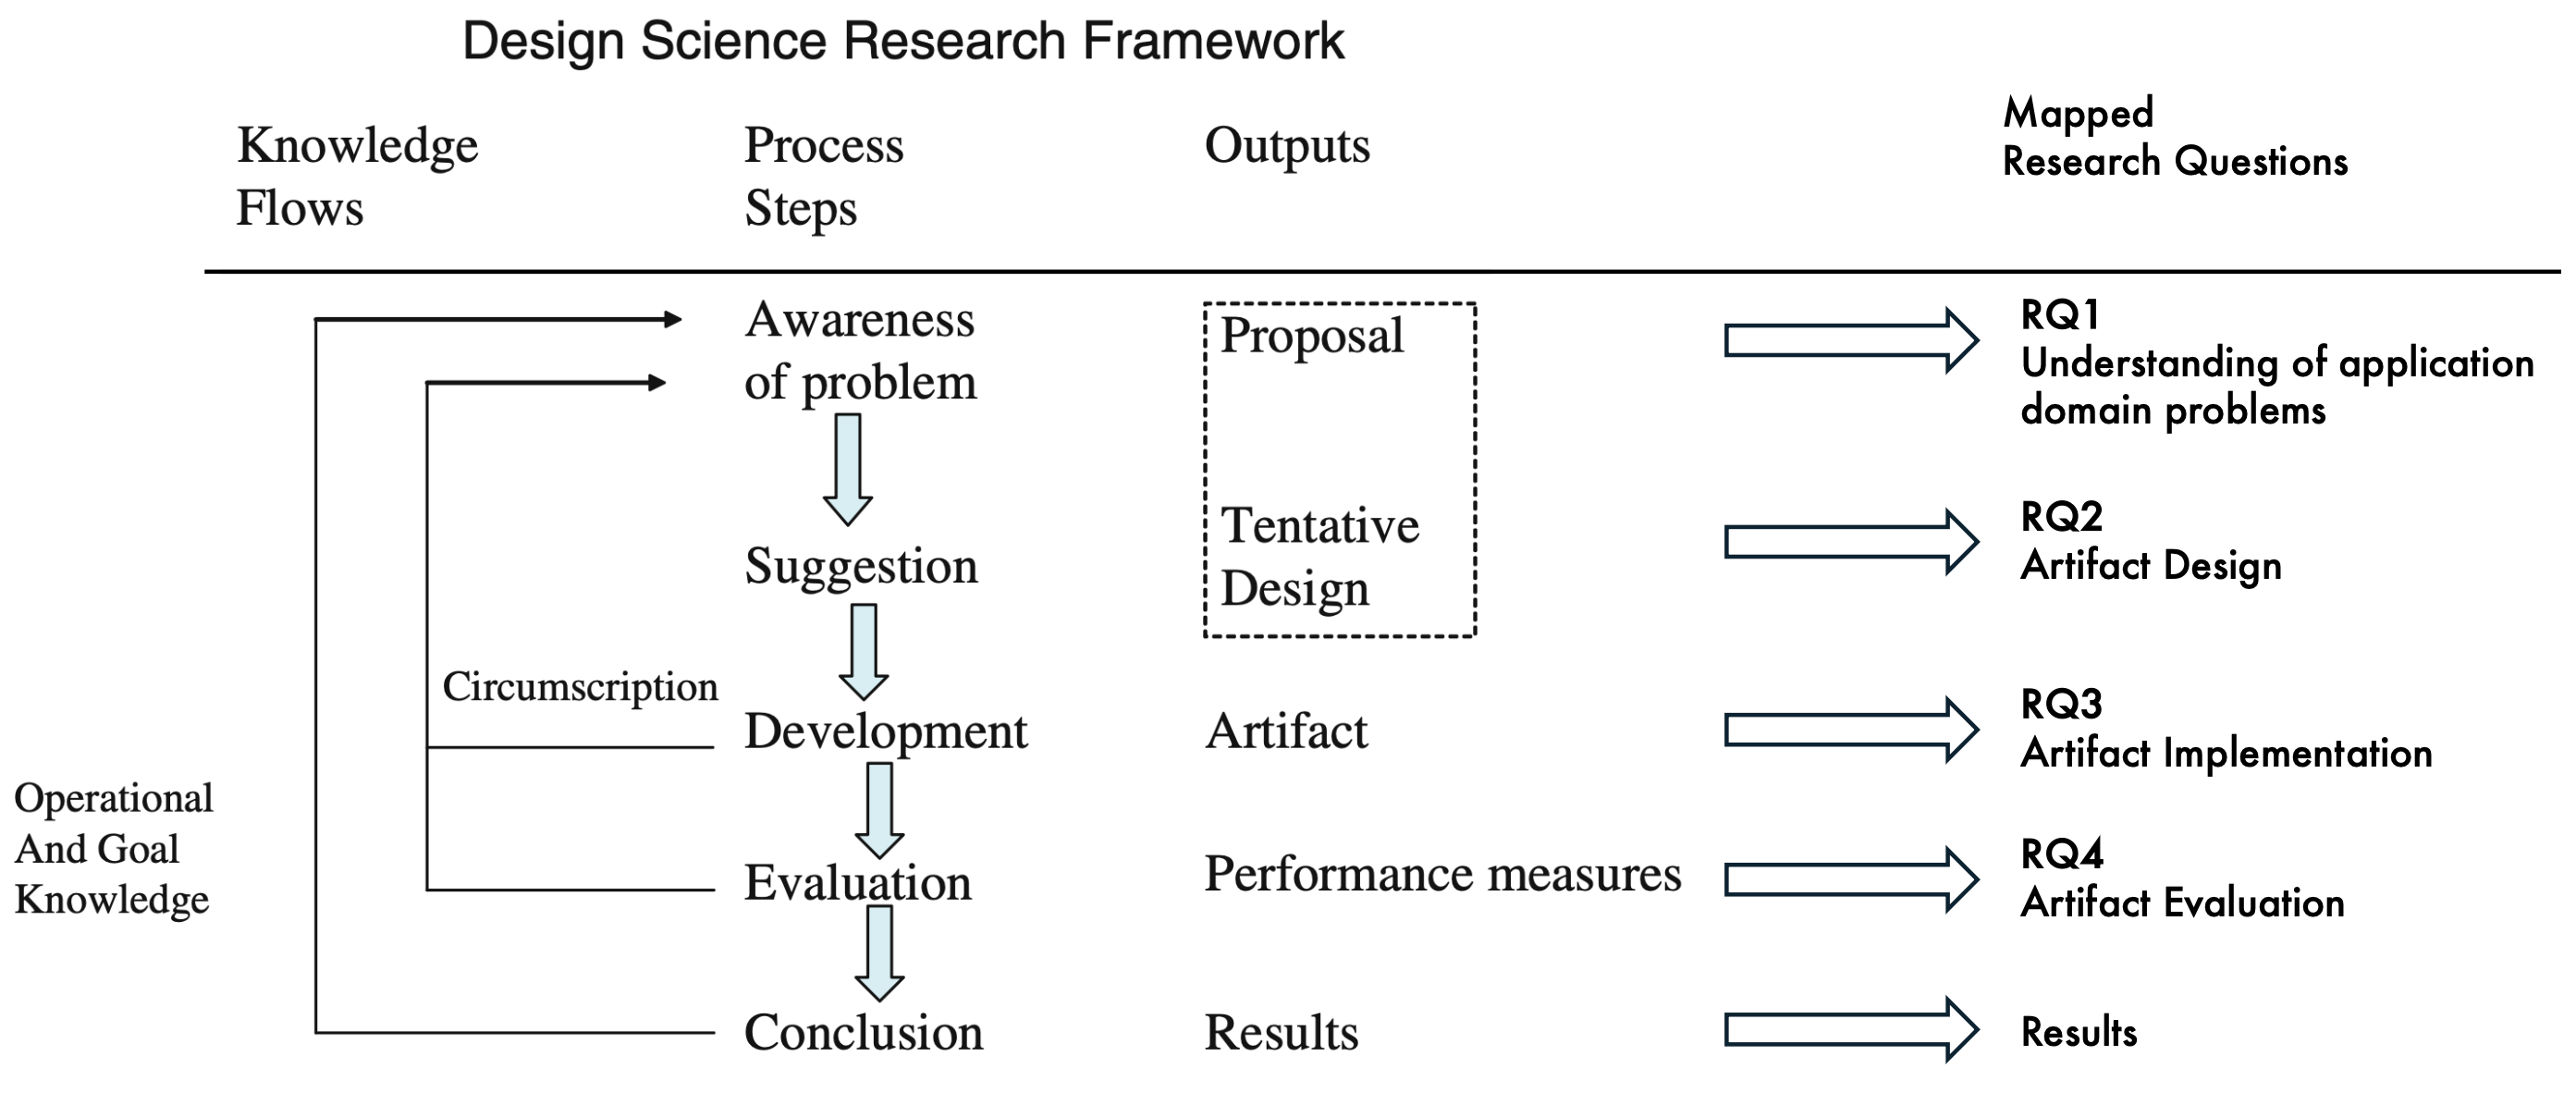
\includegraphics[width=.9\textwidth]{figures/research-design/design-science-research-framework-by-author.png}
     \rule{35em}{0.5pt}
    \caption{\acrlong{dsr} Framework adapted by the author} 
 \label{fig:design-science-research-framework-adapted-by-author}
\end{figure}


%
\section{Time Horizon}\label{sec:time-horizon}
This layer of the research onion focuses on the research's time horizon, distinguishing between longitudinal and cross-sectional approaches \cite{SaundersMark2023}.
Longitudinal research extends over an extended period, capturing multiple snapshots throughout the study.
In contrast, a cross-sectional approach examines a single snapshot within a specific, typically shorter, timeframe.
Given time constraints, this thesis adopts a cross-sectional time horizon, namely the duration of the thesis development.
%
\section{Data Collection and Data Analysis}\label{sec:data-collectiom-and-data-analysis}
Data collection is the systematic process of gathering and measuring information on specific variables to answer relevant questions and assess outcomes.
According to \textcite{SaundersMark2023}, there are four primary methods of data collection:
\begin{itemize}
    \item Questionnaires: these are an efficient way to collect data as they consist of fixed-response questions that can be easily analyzed and compared. However, a key limitation is that participants cannot clarify their answers, which may lead to misinterpretations.
    \item Interviews: interviews can be structured like questionnaires, semi-structured with a mix of predefined and open-ended questions, or unstructured, allowing the interviewer to guide the conversation. While interviews are typically conducted one-on-one, they can also be held in group settings. A major challenge is finding suitable interview participants, and there is always a risk of bias. Additionally, conducting multiple interviews can be time-consuming.
    \item Observation: in observational research, a researcher studies participants' behavior to identify patterns. While this method provides real-world insights, interpreting observations correctly and selecting appropriate subjects for observation can be challenging.
    \item Archival Research: this method involves analyzing historical documents and textual materials from organizations or institutions. It provides valuable insights from past data but may require extensive interpretation and verification.
\end{itemize}

Data analysis refers to the process that takes place after data collection, aiming to extract meaningful insights and patterns from the gathered information.

In this thesis, no questionnaires, interviews, observations, or archival research methods were employed, as the focus was strictly on the European research domain.
Given that the dataset used, detailed in the next chapter (Sec.~\ref{sec:dataset}), specifically pertains to EU-funded research projects, the analysis was conducted solely within this structured data framework, ensuring relevance to the scope of European research.
\fillingPage{}
\chapter{Scenarios Analysis}\label{chap:scenarios-analysis}
This chapter presents the scenarios used to design the proposed research collaboration recommendation system.
The scenarios are based on real data from the \gls{cordis} dataset, which contains information on EU-funded research projects.
The CORDIS dataset is described in Sec.~\ref{sec:dataset}, while Sec.~\ref{sec:scenarios} illustrates the scenario analysis of the selected European projects.
The scenarios are also used to define the application requirements (see Sec.~\ref{sec:application-requirements}) that the system must fulfil to be useful to researchers.

\section{Dataset}\label{sec:dataset}
In this study, the \gls{cordis} dataset \cite{CORDIS_FP7_2015,CORDIS_H2020_2015,CORDIS_RefData_2018} was chosen as the primary data source.
\gls{cordis}\footnote{\url{https://cordis.europa.eu}} serves as the European Commission's primary public repository for distributing information about EU-funded research projects.
This dataset is a critical resource for analyzing research trends, understanding research project collaborations, and identifying potential research partners.
The chosen dataset consists of data representations of projects funded under two major European Union research initiatives:
\begin{itemize}
    \item The \gls{fp7} for Research and Technological Development\footnote{\url{https://cordis.europa.eu/programme/id/FP7}}, covering projects funded from 2007 to 2013.
    \item The \gls{h2020} Programme for Research and Innovation\footnote{\url{https://cordis.europa.eu/programme/id/H2020}}, covering projects funded from 2014 to 2020.
\end{itemize}

The part of \gls{cordis} dataset of EU research projects under \gls{fp7}, consists of the public grant details for each project, including the following information: Record Control Number, project ID (grant agreement number), project acronym, project status, funding program, research topic, project title, start and end dates, project objectives, total project cost, maximum EC contribution (commitment), call ID, funding scheme (type of action), coordinating entity, coordinator's country, participants (listed in a semi-colon separated format), and participant countries (also in a semi-colon separated format).
\gls{fp7} organisations contains a list of participating organizations, including the following details: project Record Control Number, project ID, project acronym, organization role, organization ID, organization name, organization short name, organization type, participation status (ended: true/false), EC contribution, and the organization's country.

The part of \gls{cordis} dataset of EU research projects under \gls{h2020}, consists of six distinct subsets available in various formats:
\begin{itemize}
    \item \gls{h2020} projects: containing details on participating organisations, legal frameworks, topic classifications, project URLs, and categorization using the European Science Vocabulary.
	\item \gls{h2020} project Intellectual Property Rights: includes patent data only for granted patents that are available in the European Patent Office database.
	\item \gls{h2020} project deliverables: metadata and links to deliverables, with entries available since May 2019.
	\item \gls{h2020} project publications: metadata and links to scientific publications, included since May 2019.
	\item \gls{h2020} report summaries: periodic or final public summaries of projects, added since September 2018.
	\item Principal Investigators in \gls{h2020} ERC projects: listing key researchers involved in European Research Council projects.
\end{itemize}

\subsubsection*{Dataset Limitations}
Although the CORDIS dataset is a valuable resource for analysing research trends, project collaborations and the distribution of funding, certain limitations must be taken into account:

\begin{itemize}
	\item Data Integration Challenges: the dataset is distributed across multiple files in different formats (JSON, XML, CSV, XLSX), requiring careful preprocessing and linkage before meaningful insights can be extracted.
	Establishing relationships between different files (e.g., linking projects to participants and deliverables) is not straightforward and necessitates additional data processing steps.
	\item Inconsistent Data Representations: some fields are formatted differently in the various subsets of the data set.
	For example, project participants may be listed as semicolon-separated values in some files, while in others they appear as separate records.
	This complicates data consistency and automatic processing.
	\item Missing or Incomplete Data: some projects lack details on funding schemes, research topics, or coordinator organizations.
	Not all participant organizations have standardized names or unique identifiers, making entity resolution difficult when merging data.
	Certain project deliverables or publications might be unavailable due to proprietary restrictions or missing metadata.
\end{itemize}

\section{Scenarios}\label{sec:scenarios}
Using data from \gls{cordis}, the structures of five European research projects that are part of the \gls{h2020} programme were analysed.
The selected projects are:
\begin{enumerate}
    \item ``BIM-based holistic tools for Energy-driven Renovation of existing Residences''\label{project1}
    \item ``Integrated and Replicable Solutions for Co-Creation in Sustainable Cities''
    \item ``New integrated methodology and Tools for Retrofit design towards a next generation of ENergy efficient and sustainable buildings and Districts''
    \item ``Proactive synergy of inteGrated Efficient Technologies on buildings' Envelopes''
    \item ``Adaptive Multimodal Interfaces to Assist Disabled People in Daily Activities'' 
\end{enumerate}

All five projects analyzed follow the same structural format, including their data organization, key components, and reporting style.
Due to this uniformity, providing a detailed analysis for each project would be redundant.
Therefore, to avoid repetition and ensure clarity, only the analysis of Project \ref{project1} is presented below as a representative example.

\subsubsection*{BIM-based holistic tools for Energy-driven Renovation of existing Residences}

The BIMERR project, funded under the Horizon 2020 program, aims to develop BIM-based holistic tools for energy-driven renovation of existing residential buildings.
This research initiative focuses on digital transformation in the construction sector, particularly in building renovation, by enhancing \gls{bim} interoperability and streamlining the renovation workflow.
The project is structured around three main pages: Fact Sheet, Reporting, and Results, each of which has a distinct purpose in presenting project details, progress, and outcomes.

\paragraph*{Fact Sheet.}
It provides an overview of the BIMERR project, including its duration, objectives, keywords, programmes, topics, call for proposal, sub call, funding schemes, and consortium partners.
The project, officially titled ``BIM-based holistic tools for Energy-driven Renovation of existing Residences'', as shown in Fig.~\ref{fig:bimerr-fact-sheet}, was coordinated by Fraunhofer Gesellschaft zur F\"orderung der Angewandten Forschung EV in Germany.

\begin{figure}[htbp]
    \centering
 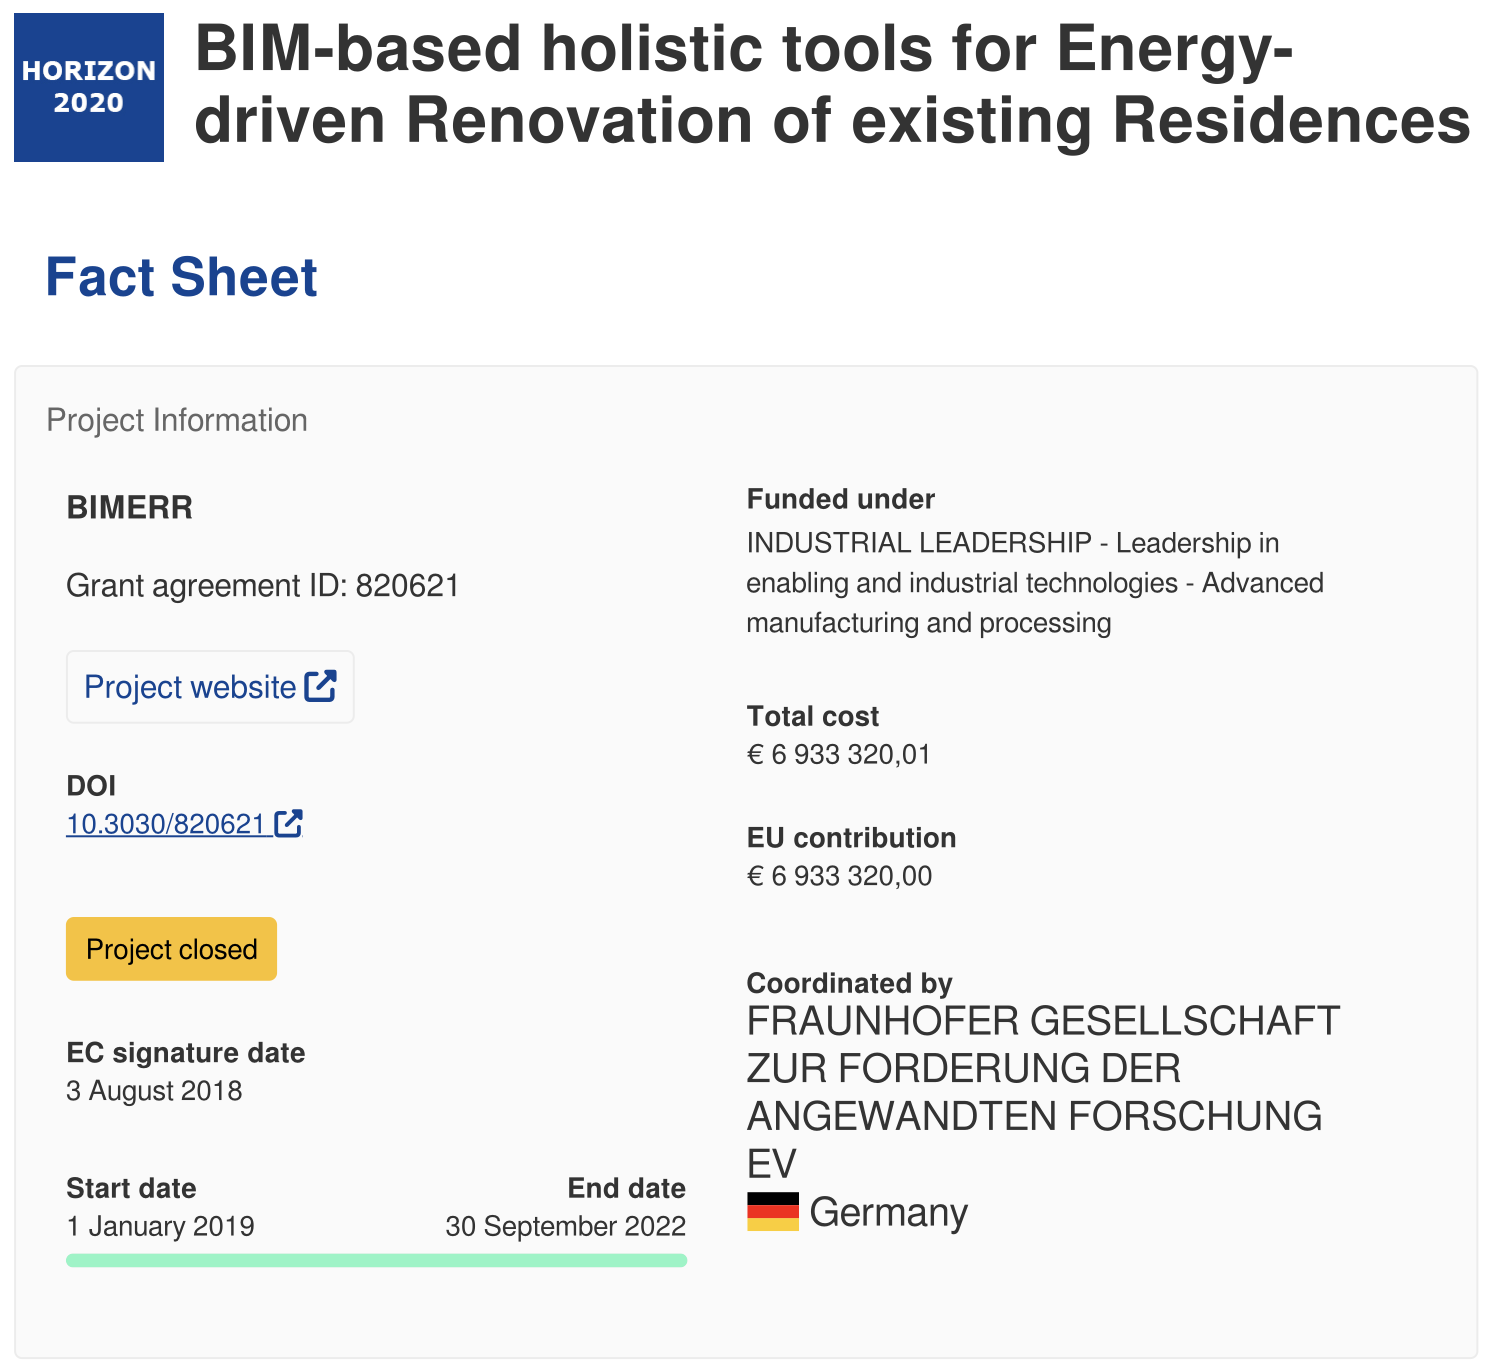
\includegraphics[width=.9\textwidth]{figures/scenario-analysis/bimerr-fact-sheet.png}
     \rule{35em}{0.5pt}
    \caption{BIMERR Project Fact Sheet}
 \label{fig:bimerr-fact-sheet}
\end{figure}

The project ran from January 1, 2019, to September 30, 2022, with a total cost of \euro 6,933,320.01, fully funded by the EU.
The Fact Sheet highlights BIMERR's key mission: developing an ICT-enabled Renovation 4.0 framework, which includes enhanced digital models of existing buildings that integrate geometrical, material, and operational data.
These models support automated scan-to-BIM, workflow modeling, and renovation decision-making.
The project aligns with the EU's energy efficiency goals by accelerating the renovation rate of buildings and improving data interoperability across various construction industry standards.
The consortium for this research project consists of 20 participants from various countries, each contributing expertise in different domains.
First of all, the coordinator, ``Fraunhofer Gesellschaft zur F\"orderung der Angewandten Forschung EV'', is based in Germany.
From Greece, the consortium includes ``Anonymos Etairia Kataskevon-Technikon Ergon, Emporikon, Viomichanikonkai Nautiliakon Epicheiriseon Kon'Kat'', ``Ethniko Kentro Erevnas Kai Technologikis Anaptyxis'', ``Hypertech (Chaipertek) Anonymos Viomichaniki Emporiki Etairia Pliroforikis Kai Neon Technologion'', ``Merit Consulting House - Olokliromenes Symvouleftikes Ipiresies Epixeiriseon Idiotiki Kefalaiouxiki Etairia'', and the ``University of Peloponnese''.
Austria is represented by ``BOC Asset Management GmbH'', and ``Xylem Science and Technology Management GmbH''.
From Poland, ``Budimex Spolka Akcyjna'' is part of the consortium.
The United Kingdom has several participants, including ``Exergy Ltd'', ``Heriot-Watt University'', ``The University of Edinburgh'', and ``University College London''.
Spain is represented by ``Ferrovial Construccion SA'' and ``Universidad Politecnica de Madrid''.
Cyprus contributes with ``Suite5 Data Intelligence Solutions Limited'' and ``Ubitech Limited''.
Belgium is represented by ``Merit Consulting House'', while Slovakia is represented by ``Novitech AS''.
Lastly, Italy is represented by ``Glassup SRL''.

\paragraph*{Reporting.}
This section documents the progress of the BIMERR project, summarizing the methodology, key objectives, and results.
The project focused on five primary objectives:
\begin{enumerate}
    \item Accelerating renovation trends through real-world pilot demonstrations in Poland and Spain.
    \item Ensuring semantic interoperability between different \gls{bim} and construction data models.
    \item Developing automated tools for converting real-world buildings into digital \gls{bim} models.
    \item Providing decision-support tools for various renovation stakeholders.
    \item Encouraging the adoption of BIMERR technologies through outreach and standardization efforts.
\end{enumerate}

The tangible outputs of BIMERR include:
\begin{itemize}
    \item BIMERR Data Models and Ontologies, ensuring compatibility with industry standards.
    \item BIMERR Middleware, enabling seamless communication between renovation tools.
    \item Scan-to-BIM Tools, supporting automatic conversion of physical buildings into digital \gls{bim} models.
    \item Augmented Reality Applications, tools such as ARIBFA for onsite \gls{bim} model visualization and BICA, a smartphone application for building residents to contribute renovation insights.
    \item Renovation Decision Support System, assisting stakeholders in selecting energy-efficient renovation strategies.
    \item Process and Workflow Management Toolkit, tools for modeling, simulation, and automation of renovation tasks.
\end{itemize}
	
The Reporting page also details BIMERR's evaluation and commercialization strategy, outlining efforts to transition project outputs into market-ready solutions (TRL9).
A preliminary business plan and financial model were developed to explore commercialization via joint ventures and external funding sources.

\paragraph*{Results.}
The last section provides access to deliverables, reports, and demonstrators generated during the project.
The page links to 22 project reports, including:
\begin{itemize}
    \item BIMERR System Architecture
    \item Best practice examples of BIMERR use
    \item Pilot site evaluations
    \item Standardization and interoperability reports
    \item Stakeholder engagement reports
    \item Impact assessments and performance evaluations
\end{itemize}

Additionally, the Results page features demonstrators, pilots, and prototypes of the BIMERR tools, including:
\begin{itemize}
    \item BIMERR Interoperability Framework, a cloud-based platform facilitating seamless data exchange.
    \item AI-Enabled Scan-to-BIM Tools, using smart glasses for on-site digital building model annotation.
    \item Adaptive Workflow Management Tools, automating and optimizing renovation processes.
    \item Building Energy Modeling and Life Cycle Assessment Modules, estimating energy efficiency and cost-effectiveness of renovations.
    \item Urban Planning Modules, integrating renovation decisions with broader urban development plans.
\end{itemize}

Furthermore, the publications and dissemination materials produced by the BIMERR consortium include:
\begin{itemize}
    \item 19 peer-reviewed articles
    \item Conference papers and workshop presentations
    \item Social media outreach and newsletters
    \item Training materials for industry adoption
\end{itemize}

\section{Application Requirements}\label{sec:application-requirements}
As an output of this analysis a list of \glspl{appr} has been derived.
Each project was part of the Research and Innovation Action funding scheme and focused on \gls{bim} as the main topic.
In the following we report a short list of the main \glspl{appr}: the project description (\gls{appr}1), objectives (\gls{appr}2), field of science, programmes, topics, proposal call, funding scheme, and keywords (\gls{appr}3).
In addition, there are the most important details concerning the coordinating organisation (\gls{appr}4) of the project, and all the organisations participating (\gls{appr}5) in that project.
Each organisation presents secondary information such as postal address, location (\gls{appr}6), and main type of activity.
The available information only concerns organisations.
However, for the recommendation of collaborators it is important to also know which people from the relevant organisations are involved in the projects, therefore we considered it as an additional requirement (\gls{appr}7).
Table \ref{tab:application-requirements} shows the list of \glspl{appr} and their corresponding description.

\begin{table}[htbp]
    \centering
    \scriptsize
    \begin{tabularx}{\textwidth}{|>{\centering\arraybackslash}p{2cm}|X|}
      \hline
      \textbf{Application Requirement} & \textbf{Description}\\
        \hline
        \gls{appr}1 & Project Description \\
        \gls{appr}2 & Objectives \\
        \gls{appr}3 & Field of Science, Programmes, Topics, Proposal Call, Funding Scheme, Keywords \\
        \gls{appr}4 & Coordinating Organisation \\
        \gls{appr}5 & Participating Organisations \\
        \gls{appr}6 & Postal Address, Location, Main Type of Activity \\
        \gls{appr}7 & People involved in the projects \\
        \hline
    \end{tabularx}
    \caption{List of \acrfullpl{appr} and their corresponding description}
    \label{tab:application-requirements}
\end{table}
        
\fillingPage{}
\chapter{A Knowledge-Driven and Hybrid AI Architecture for Research Collaboration}\label{chap:Knowledge-DrivenArchitecture}
This chapter presents the architecture of the research collaboration recommender system, which is based on a hybrid \gls{ai} approach.
First of all, the ontology selection process is described in Sec.~\ref{sec:ontology-selection}.
Then, the recommendation strategy is presented in Sec.~\ref{sec:recommendation-strategy}.
Finally, the architecture design is detailed in Sec.~\ref{sec:architecture-design}.


\section{Ontology Selection}\label{sec:ontology-selection}
In the problem awareness phase, we addressed the first sub-research question:
\begin{center}
    \rqOne
\end{center}
To establish a foundation for this study, we conducted a comprehensive literature review covering key areas such as research collaboration (Sec.~\ref{sec:research-collaboration}), the role of \acrlongpl{kg} and ontologies in the research domain (Sec.\ref{sec:knowledge-graphs}), \acrlongpl{llm} and their applications (Sec.~\ref{sec:large-language-models}), \acrlongpl{rag} concepts and approaches (Sec.~\ref{sec:retrieval-augmented-generation}), recommender systems tailored for research contexts (Sec.~\ref{sec:recommender-systems-in-research-field}), and the emerging field of Retrieval-Augmented Recommender Systems (Sec.~\ref{sec:retrieval-augmented-recommender-systems-in-research-field}).
From the literature review conducted, existing \glspl{kg} in the research field, such as \gls{mag}, \gls{s2ag}, Wikidata, \gls{orkg}, and VIVO ontology, were analyzed.
However, these \glspl{kg} and ontologies, present several limitations that impact their effectiveness in research collaborator recommendation such as:
\begin{itemize}
    \item Lack of granular and up-to-date data: many of these \glspl{kg} rely on static datasets or periodic updates, making it challenging to capture evolving research trends, emerging collaborations, and newly published work in real time.
    \item Limited contextual understanding: while these \glspl{kg} store structured information about authors, affiliations, and citations, they often lack deeper semantic connections, such as researchers' interdisciplinary expertise, project alignments, or implicit collaboration potential.
    \item Explainability and interpretability issues: many existing \glspl{kg} focus on metadata-level relationships rather than explaining why certain collaborations might be beneficial. This limits their ability to support explainable \gls{ai}-driven recommendations.
    \item Integration challenges: despite leveraging \gls{lod} principles, these \glspl{kg} are often designed with distinct schemas and ontologies, leading to interoperability challenges when combining multiple sources for enriched recommendations.
\end{itemize}

Given these limitations, the \gls{eurio} \gls{kg} was identified as particularly suitable for modeling European projects, making it an excellent choice for this thesis.
\gls{eurio} provides structured, rich metadata on European-funded projects, including participants, topics, and collaborations.
By leveraging \gls{eurio}, this thesis aims to overcome the limitations of existing \glspl{kg}, enabling a more dynamic, explainable, and semantically enriched recommendation framework.
The \gls{eurio} ontology and \gls{kg} are described in the following subsections.

Moreover, we found that most of the papers analyzed on recommender systems in the research domain, are designed to suggest research papers or to recommend collaborators.
In both cases, the most relevant aspects on which the recommender algorithms are based are influences on the number of citations, and abstracts of the papers.
Despite their advancements, recommender systems face significant limitations, particularly in complex domains like research collaboration.
Traditional methods such as \gls{cbf} and \gls{cf} suffer from data sparsity, making accurate recommendations difficult when user interaction data is limited.
The cold-start problem further complicates this by preventing effective suggestions for new users or items.
Additionally, many systems lack explainability, reducing user trust and interpretability, especially in critical decision-making contexts.
Another challenge is the tendency to prioritize historical patterns over novel discoveries, restricting interdisciplinary connections.
These limitations underscore the need for knowledge-aware recommender systems that integrate domain-specific semantics, contextual understanding, and explainable \gls{ai} techniques to enhance recommendation quality, fairness, and effectiveness.
We will focus on the identified research gap, which is in the limitations of \gls{dl}-based recommendation systems in capturing users' preferences, handling diverse textual information, and providing explainable recommendations.
These models often struggle to generalize to unseen scenarios and lack interpretability, making them less effective for tasks that require complex reasoning, such as recommendations from research collaborators.

\subsection*{EURIO: EUropean Research Information Ontology}
The \gls{eurio} ontology, developed by the Publications Office of the European Union\footnote{\url{https://op.europa.eu/en/}}, is a data model which conceptualizes, formally encodes, and makes available in an open, structured, and machine-readable format data about research projects funded by the EU's framework programmes for research and innovation.
\gls{cordis}, as described in Sec.~\ref{sec:dataset}, is responsible for publishing the results of these projects, while \gls{eurio} provides a semantic model that enhances transparency, reusability, and accessibility.
\gls{eurio} is built on top of well-known ontologies and vocabularies to ensure interoperability and semantic richness.
These include:
\begin{itemize}
    \item \gls{dc}: used for metadata elements such as titles, descriptions, and identifiers.
    \item \gls{dcat}: an \gls{rdf} vocabulary designed to facilitate interoperability between data catalogs published on the Web.
    \item \gls{dingo}: an ontology expressly designed to provide an extensible interoperable framework for formally conceptualizing and expressing the relevant parts of the research/cultural landscape in relation to funding, such that they can easily be shared between different actors and platforms.
    \item \gls{fabio}: facilitates the description of bibliographic entities and their relationships.
    \item \gls{frapo}: an ontology for describing the administrative information of research projects, e.g., grant applications, funding bodies, project partners, etc.
    \item \gls{foaf}: defines relationships between people and organizations.
    \item \gls{skos}: facilitates controlled vocabularies and classification schemes.
\end{itemize}

The \gls{eurio} ontology also incorporates reference data, such as countries, funding schemes, types of action, the EuroSciVoc taxonomy, and the NUTS classification, to enhance the semantic representation of research information.
It leverages the \gls{owl} 2 to formally define the semantics of domain-specific terms used to describe \gls{cordis} entities (e.g., projects, organizations, etc.), their attributes (e.g., title, acronym, legal name, etc.), and their interrelations (e.g., the connection between a project and its participating organizations, etc.).

\gls{eurio} defines multiple classes representing different concepts such as projects, organizations, funding schemes, grants, publications, and roles, along with associated data properties and object properties that define their relationships.
Each class has a set of data properties that describe its attributes, and a set of object properties that define its connections to other classes.
Each class, data property, and object property has several annotations but in general the main annotations for those are \textit{rdfs:label}, which provides a human-readable label for the entity, \textit{rdfs:comment}, which provides a human-readable description of the entity, and \textit{rdfs:isDefinedBy}, which provides a link to the ontology where the entity is defined.

For example, the title, description, start date, end date, and funding amount are data properties of the \textbf{Project} class.
The ontology also defines relationships between classes, such as \textbf{is funded by}, the association between a project and its grant (Fig.~\ref{fig:is-funded-by}).

\begin{figure}[htbp]
    \centering
 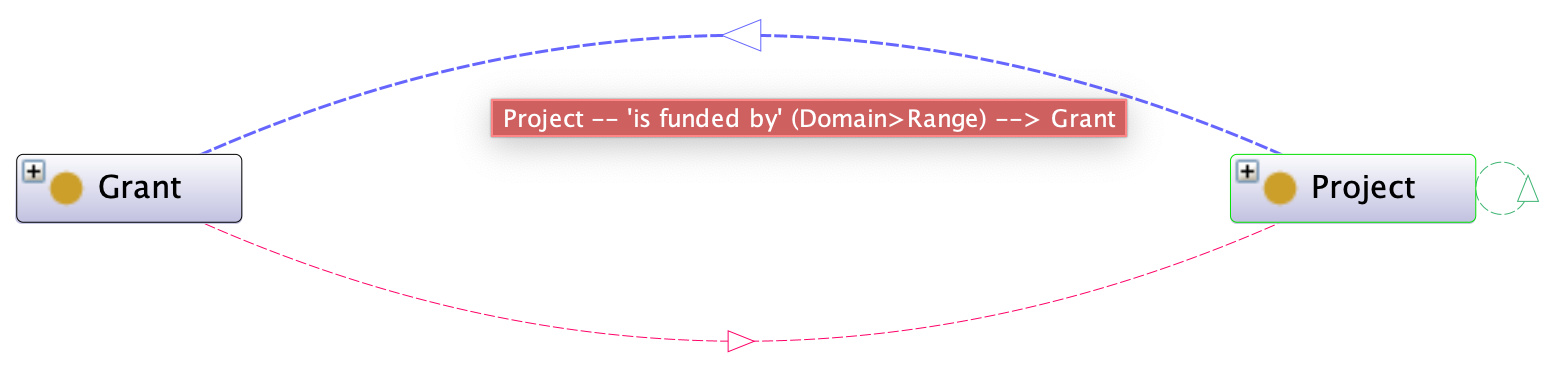
\includegraphics[width=.9\textwidth]{figures/architecture/is-funded-by.png}
     \rule{35em}{0.5pt}
    \caption{The ``is funded by'' relationship between a project and its grant}
 \label{fig:is-funded-by}
\end{figure}

Another example or relationship is \textbf{is employed by}, which links a person, in particular a \textbf{Person Role} to an \text{Organisation}.
The ontology also provides object property descrptions, for example the \textbf{has involved party} relationship, which links a \textbf{Project} to a \textbf{Role}, is inverse of \textbf{is involved in}, which links a \textbf{Role} to a \textbf{Project} (Fig.~\ref{fig:is-involved-in-has-involved-party}).

\begin{figure}[htbp]
    \centering
 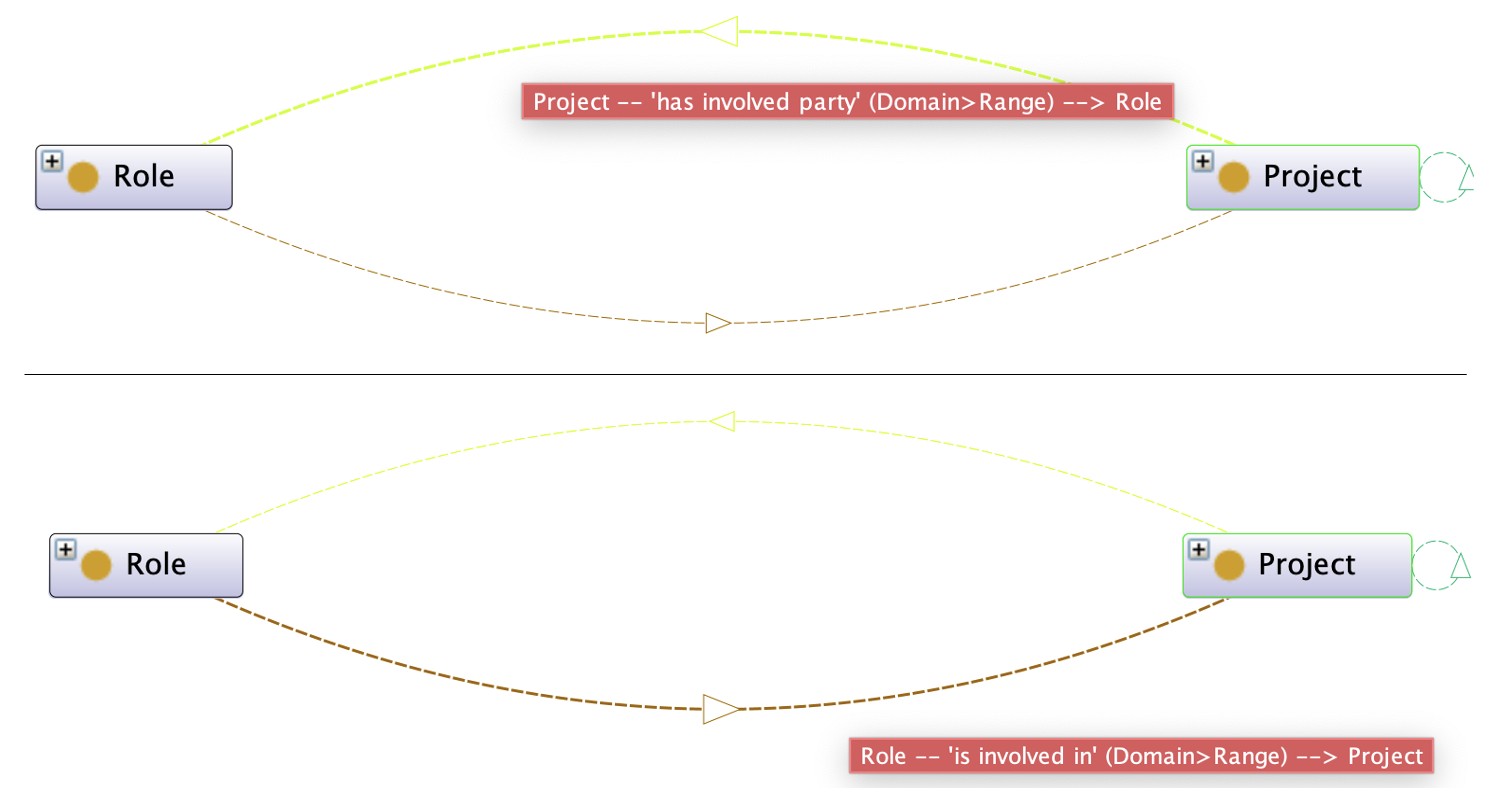
\includegraphics[width=.9\textwidth]{figures/architecture/has-involved-party-is-involved-in.png}
     \rule{35em}{0.5pt}
    \caption{The ``has involved party'' and ``is involved in'' relationships}
 \label{fig:is-involved-in-has-involved-party}
\end{figure}
\newpage
This object property descriptions can be very useful for querying the \gls{kg} to extract relevant information in a structured manner.
Moreover, the ontology defines a hierarchy of classes.
For example, the \textbf{Organisation} class is a superclass of several subclasses such as \textbf{For Profit Organisation}, \textbf{Funding Agency}, \textbf{Higher Or Secondary Education}, \textbf{Research Organisation}, and \textbf{SME} (Small and Medium Enterprise) (Fig.~\ref{fig:organisation-class-hierarchy}).

\begin{figure}[htbp]
    \centering
 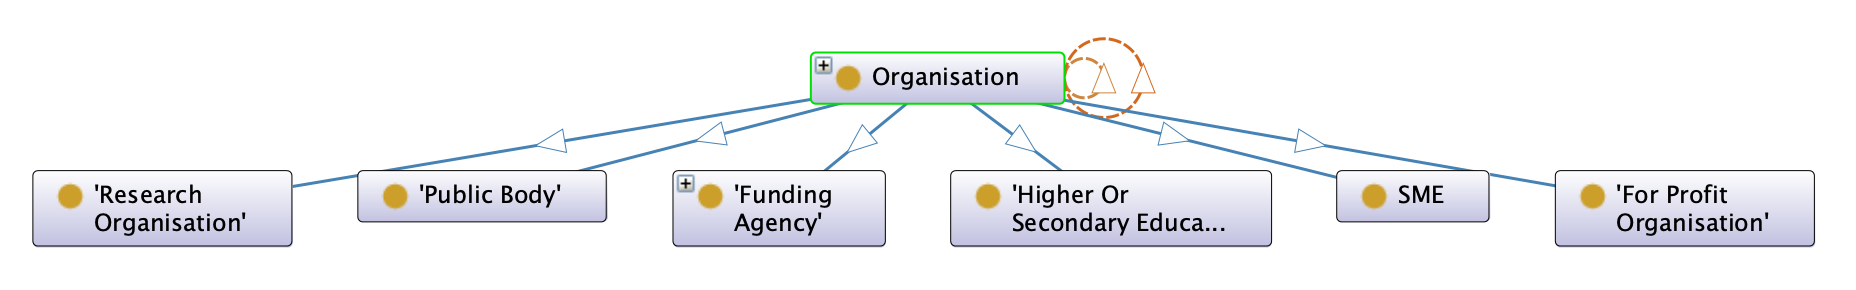
\includegraphics[width=.9\textwidth]{figures/architecture/organisation-class-hierarchy.png}
     \rule{35em}{0.5pt}
    \caption{The ``Organisation'' class hierarchy}
 \label{fig:organisation-class-hierarchy}
\end{figure}

An overview of the \gls{eurio} ontology is shown in the UML diagram in Fig.~\ref{fig:eurio-ontology}.

\begin{figure}[htbp]
    \centering
 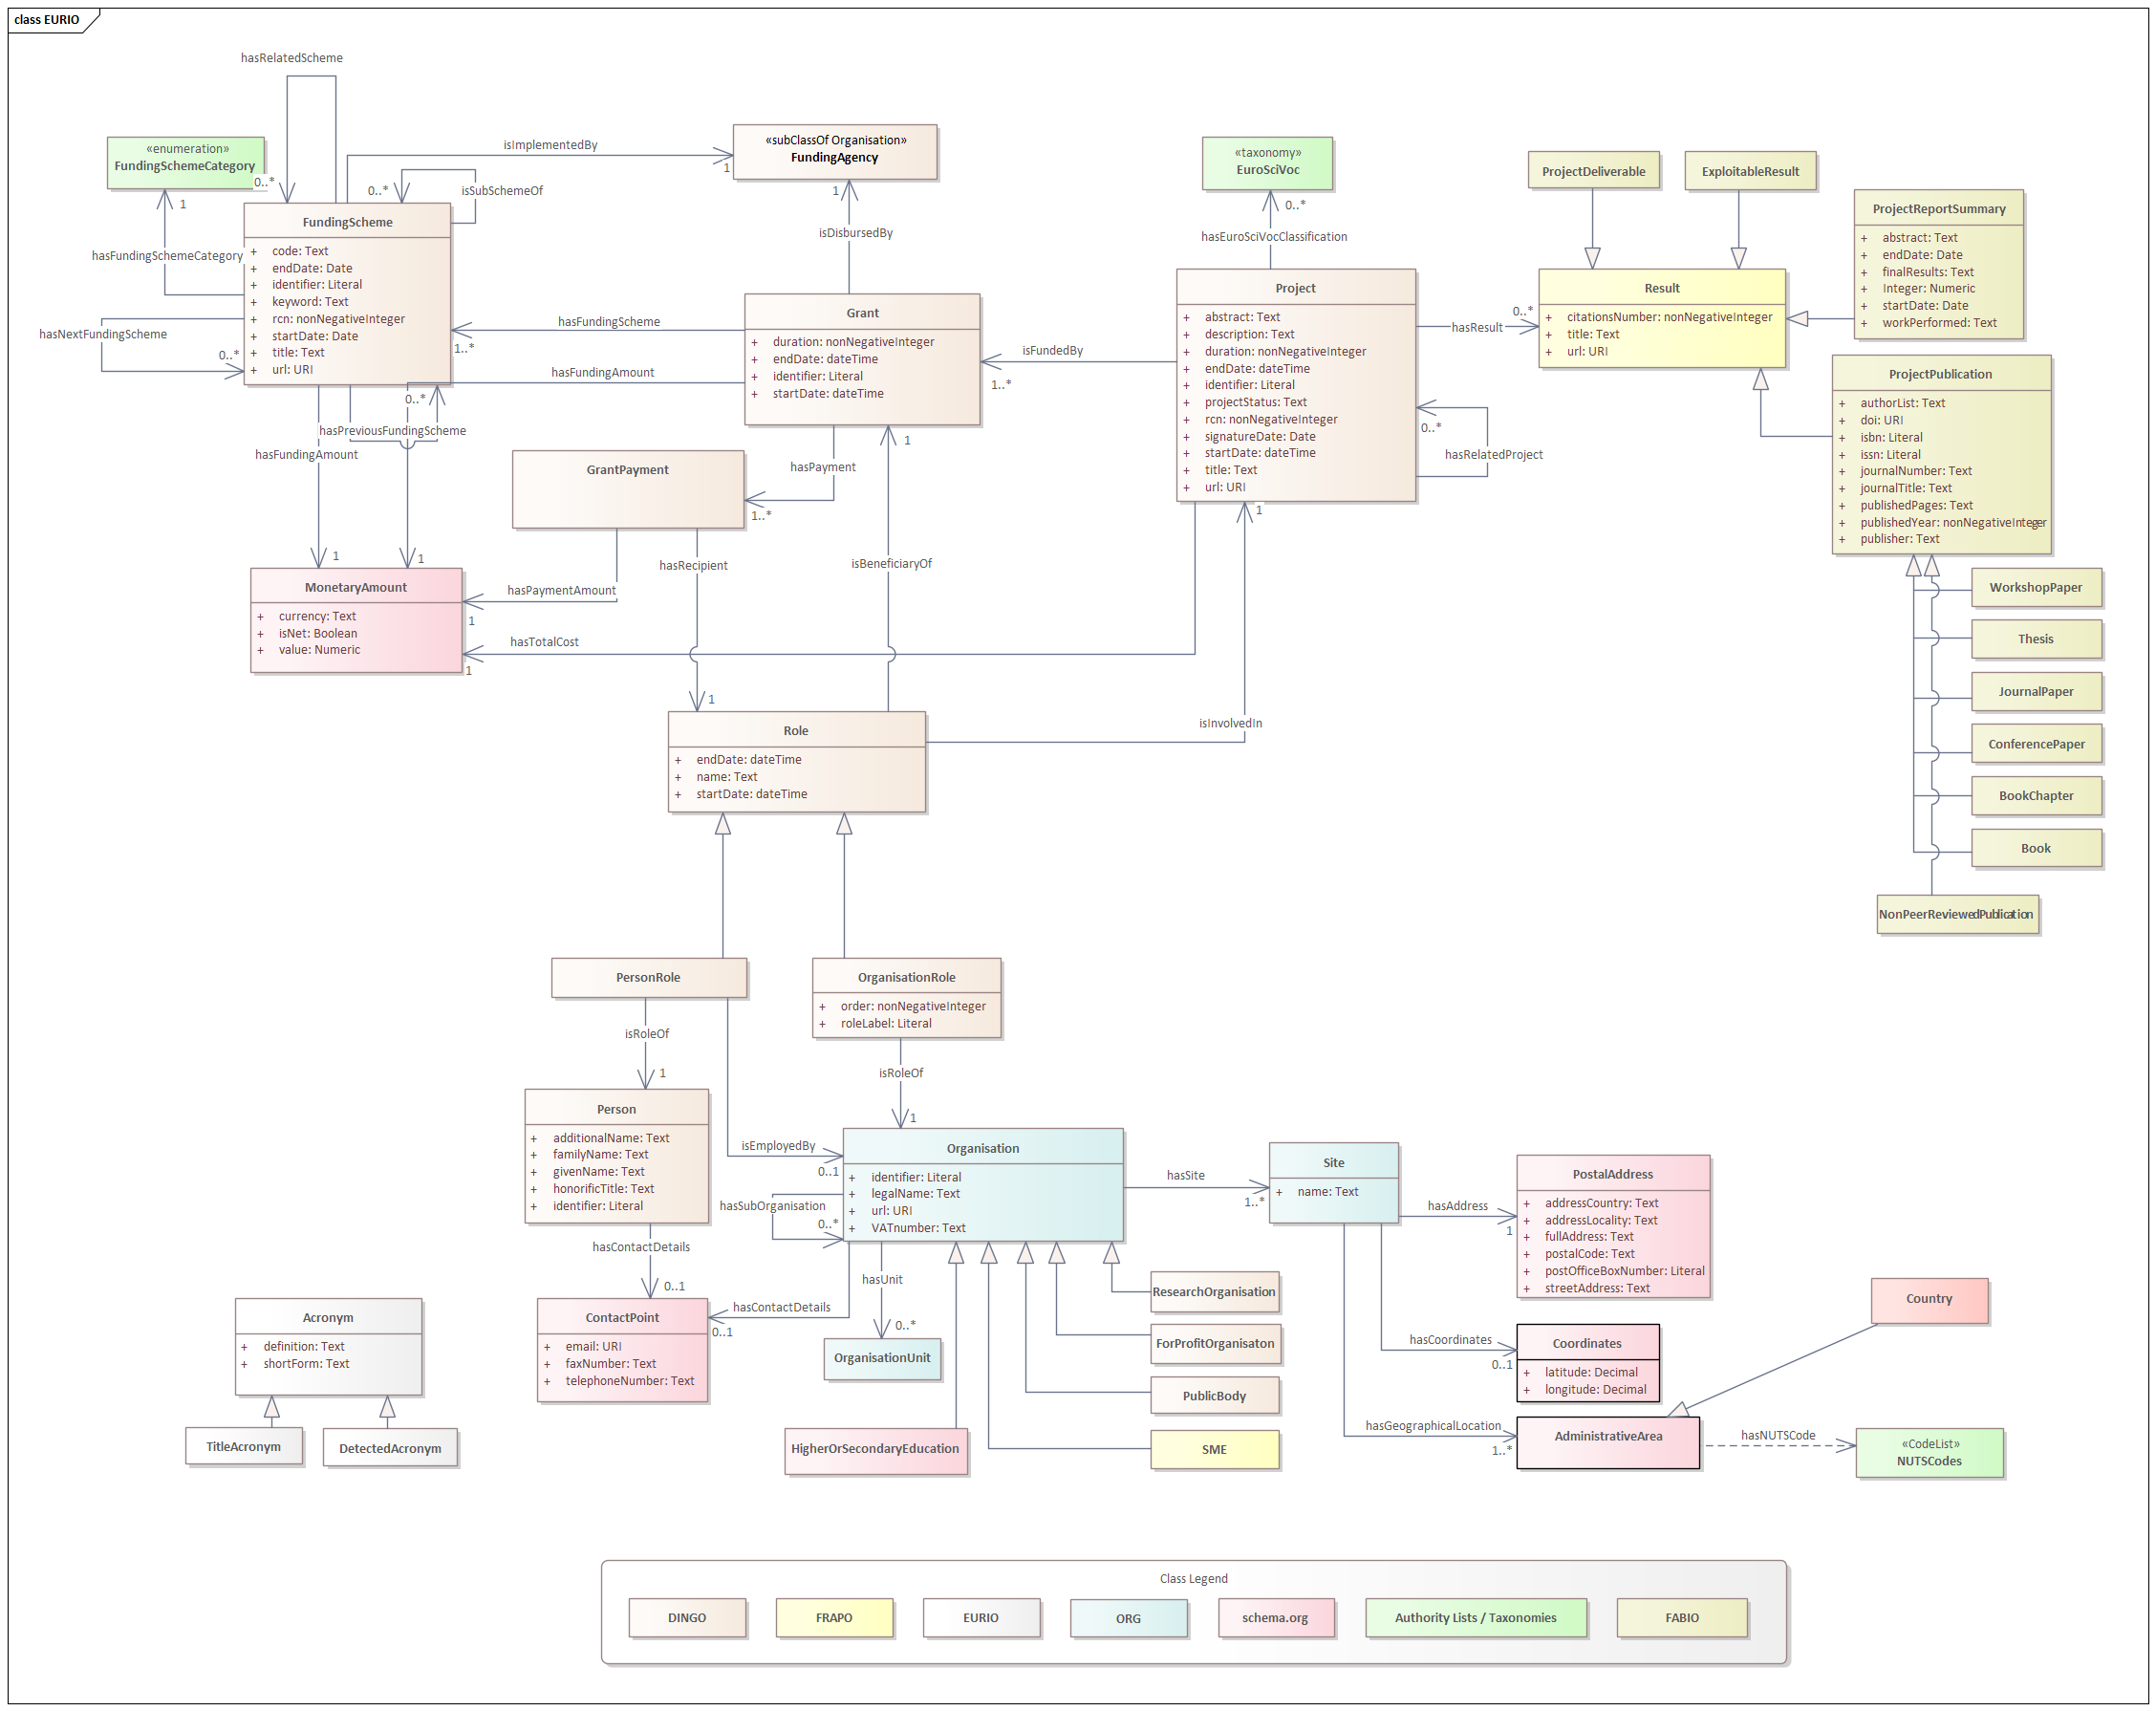
\includegraphics[width=\textwidth]{figures/architecture/EURIO_V2.4.png}
     \rule{35em}{0.5pt}
    \caption{A graphical representation of the \gls{eurio} ontology (from \url{https://op.europa.eu/en/web/eu-vocabularies/eurio})}
 \label{fig:eurio-ontology}
\end{figure}
\newpage

\subsection*{Data Availability and Formats}
The dataset is structured in \gls{rdf} format and contains over 18 million \gls{rdf} triples, with a total size of approximately 5GB when serialized in the N-Quad Triples \gls{rdf} format.
These structured triples enable the representation of relationships between projects, organizations, researchers, project publications, funding schemes, grants, countries, and other relevant entities making, the dataset a rich resource for \gls{kg}-based research.

The \gls{eurio} \gls{kg} is available in multiple formats to ensure accessibility and ease of integration into different research workflows.
Supported formats include \gls{rdf}, \gls{ttl}, \gls{nq}, \gls{jsonld}, and \gls{nt}.
The \gls{eurio} \gls{kg} used in this thesis is the latest version updated by the European Union on 08.11.2023, ensuring that the data remains relevant and accurate up to this date.

\section*{Knowledge Graph Exploration}
As previously explained, the \gls{eurio} \acrlong{kg} \cite{CORDIS_EURIO_2022} is built upon \gls{cordis} data and serves as a structured \gls{kg} that encapsulates information about research projects funded under the \gls{fp7} and \gls{h2020} framework programmes.
The \gls{eurio} \gls{kg} can be accessed via a \gls{sparql} endpoint at \url{https://cordis.europa.eu/datalab/sparql-endpoint/en}.
The \gls{kg} provides both database dumps and subsets of \gls{eurio} data in the form of named graphs.
The structure and organization of these named graphs are defined by the \gls{eurio} ontology, which is publicly available at: \url{https://op.europa.eu/en/web/eu-vocabularies/eurio}.

As part of this study, we conducted an exploration of the \gls{eurio} \gls{kg}, focusing on analyzing and understanding its ontology schema by identifying and examining the most important concepts, relationships, and structural elements.
This initial exploration allowed us to gain insights into the way projects, organizations, researchers, and related entities are modeled within the dataset.
For example, the Fachhochschule Nordwestschweiz and University of Camerino  subgraphs were extracted from the \gls{eurio} \gls{kg} to understand their properties and relationships.
Figures~\ref{fig:fhnw-graphdb} and~\ref{fig:unicam-graphdb} show the subgraphs for Fachhochschule Nordwestschweiz and University of Camerino, respectively, highlighting the connections between other entities.

\begin{figure}[htbp]
    \centering
 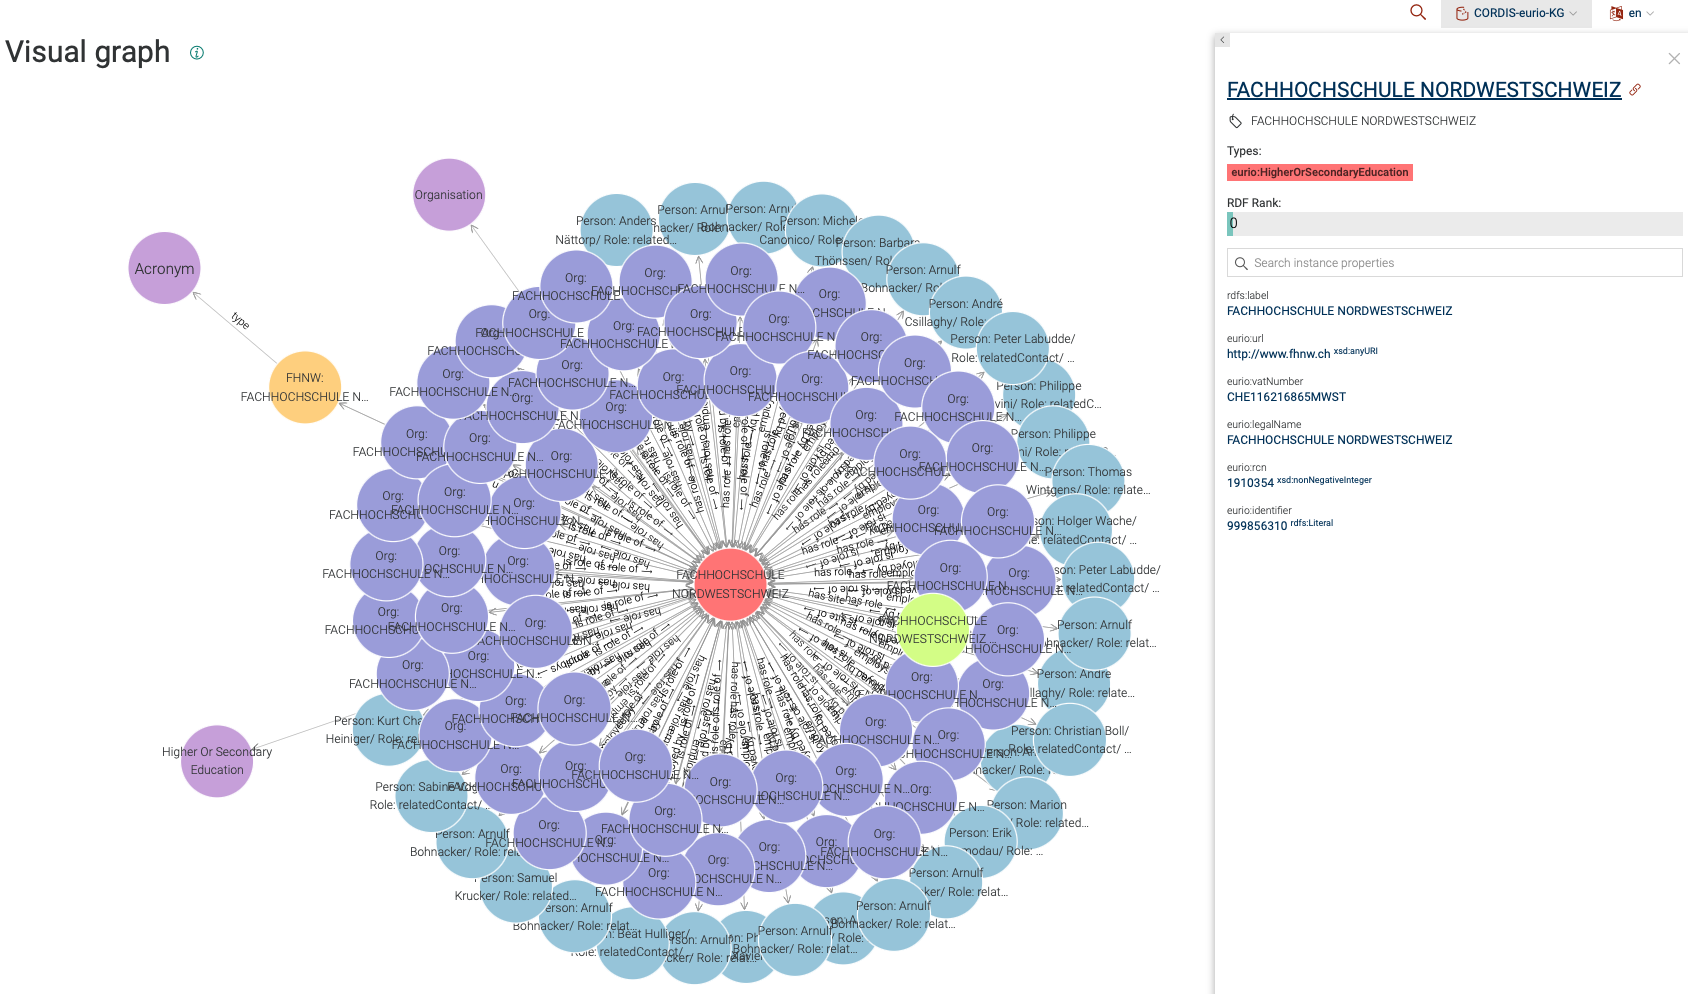
\includegraphics[width=.9\textwidth]{figures/architecture/graphdb-fhnw.png}
     \rule{35em}{0.5pt}
    \caption{FACHHOCHSCHULE NORDWESTSCHWEIZ subgraph in the \gls{eurio} \gls{kg}}
 \label{fig:fhnw-graphdb}
\end{figure}

\begin{figure}[htbp]
    \centering
 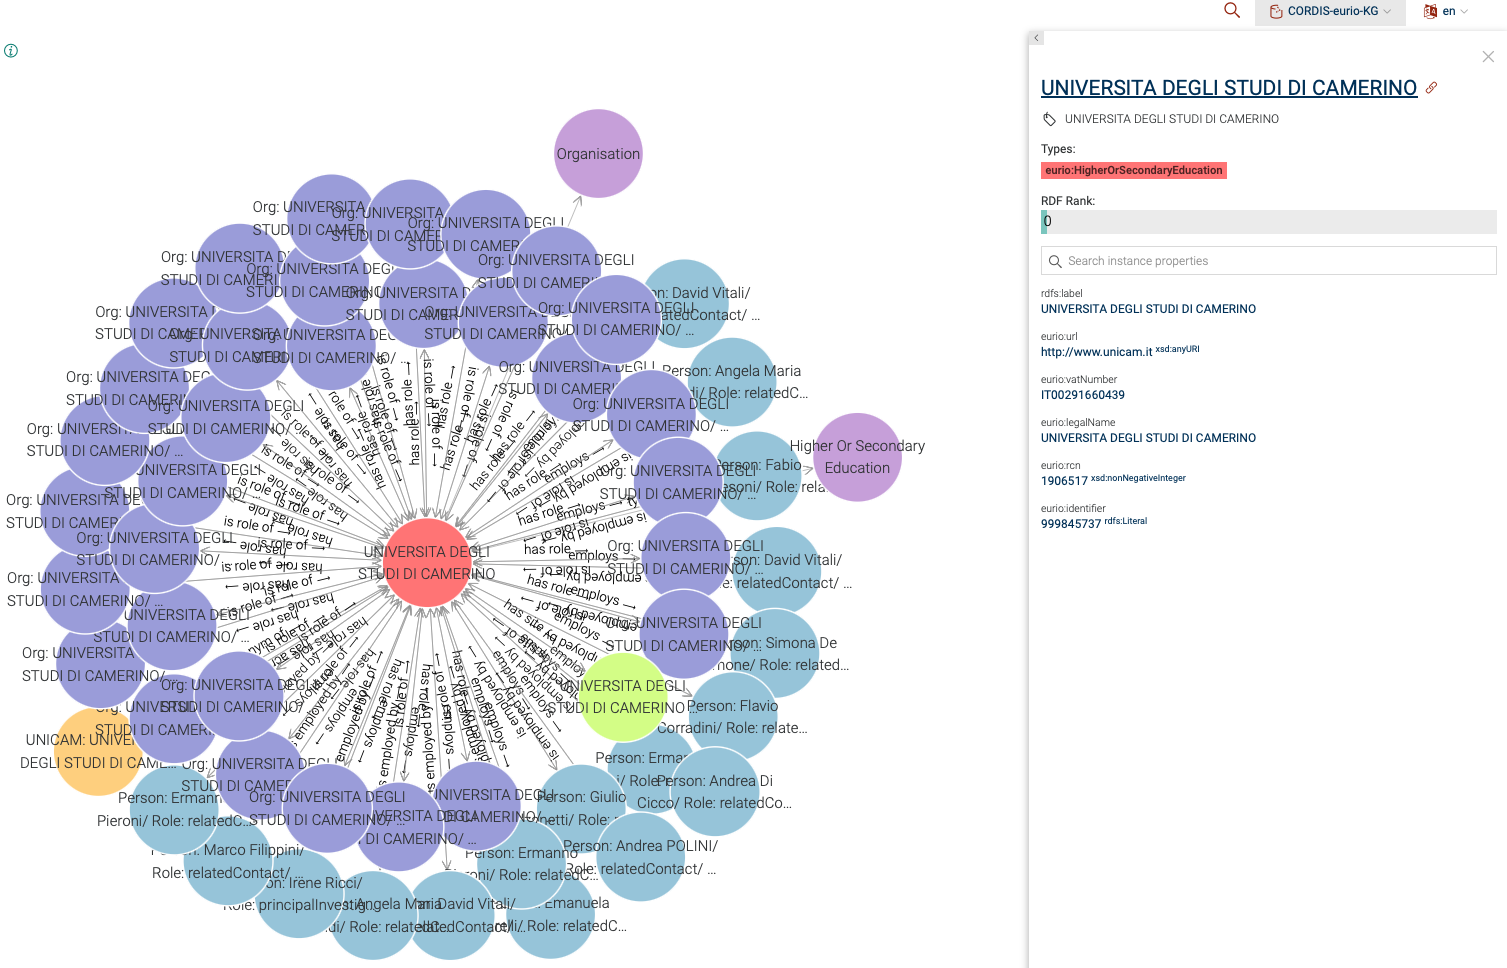
\includegraphics[width=.9\textwidth]{figures/architecture/graphdb-unicam.png}
     \rule{35em}{0.5pt}
    \caption{University of Camerino subgraph in the \gls{eurio} \gls{kg}}
 \label{fig:unicam-graphdb}
\end{figure}
\newpage
As can be seen from both figures, both the Fachhochschule Nordwestschweiz and the University of Camerino are instances of the \textbf{eurio:HigherOrSecondaryEducation} class and have the following six data properties: \textit{rdfs:label}, \textit{eurio:url}, \textit{eurio:vatNumber}, \textit{eurio:legalName}, \textit{eurio:rcn}, and \textit{eurio:identifier}.
Furthermore, we can see that, taking Fachhochschule Nordwestschweiz as an example, it has several \textit{eurio:hasRole} relationships with different ``Org: FACHHOCHSCHULE NORDWESTSCHWEIZ'' entities.
The \gls{kg} contains several such redundancies, also for other types of classes.
Each entity of type \textbf{eurio:Organisation} has several relationships with the entity of type \textbf{eurio:OrganisationRole}.
This type of relationship implies a lot of redundancy in the nodes of the \gls{kg}, but is deduced to be necessary to represent the project-related organisation role.
For example, as illustrated in Fig.~\ref{fig:fhnw-organisationRole-example}, the Fachhochschule Nordwestschweiz node is linked via the \textit{euro:hasRole} relationship, to the node ``Org: FACHHOCHSCHULE NORDWESTSCHWEIZ/ Role: participant/ Project: 53135'', which semantically represents the participation of the Fachhochschule Nordwestschweiz in the project with project ID 53135.
From the data properties of this node, we can easily see that the role of the FHNW in this project was participant, and that the project duration was from April 4, 2018, to September 30, 2021.

\begin{figure}[htbp]
    \centering
 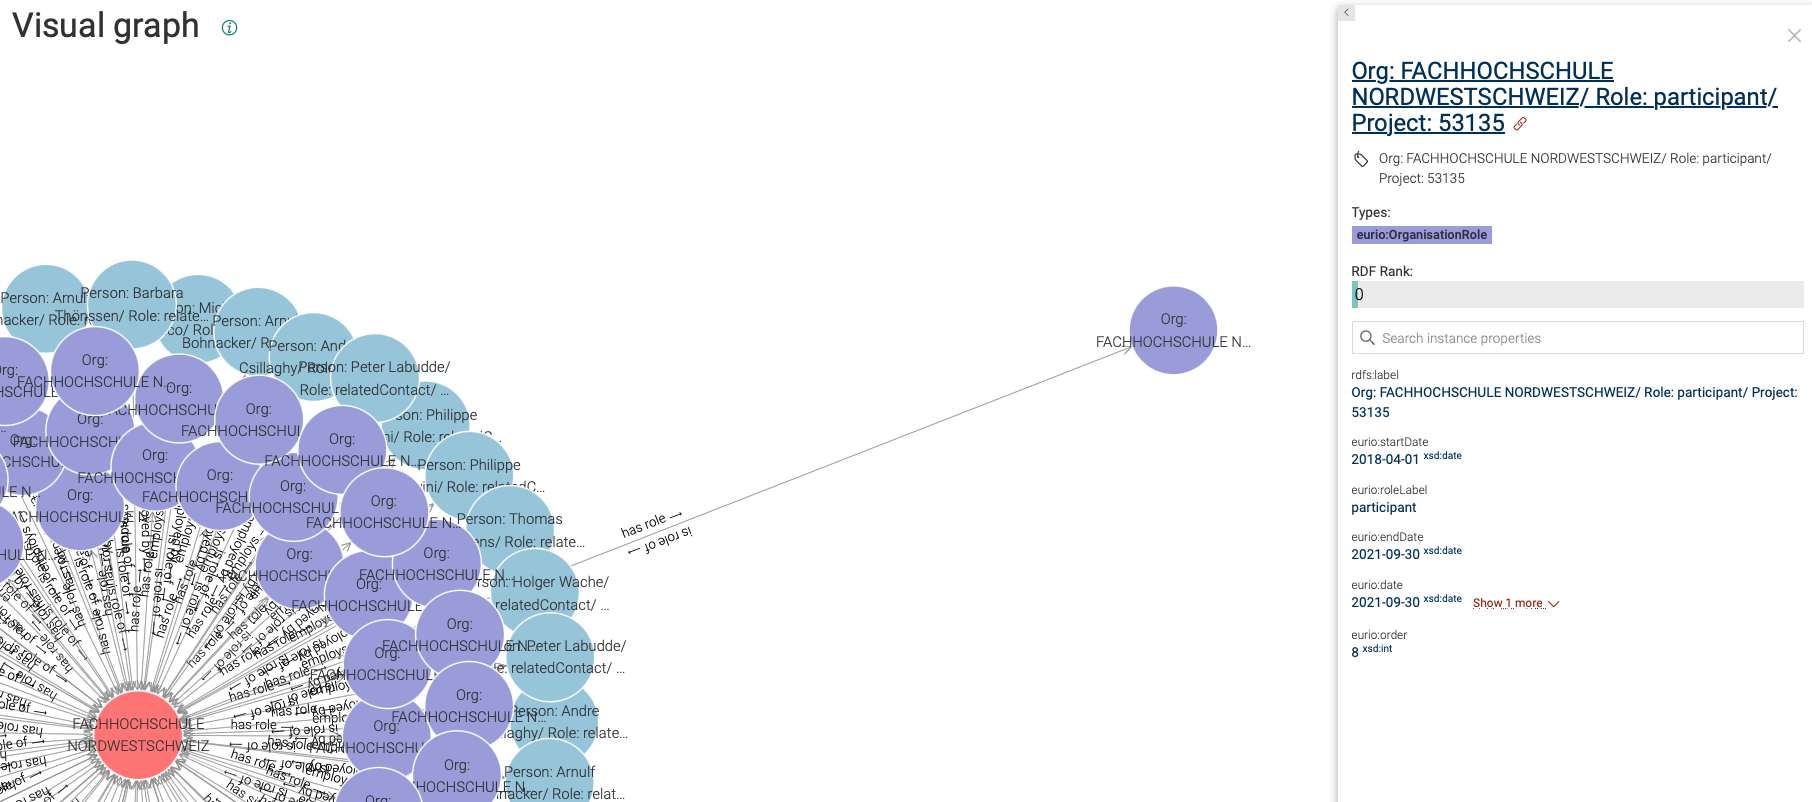
\includegraphics[width=.9\textwidth]{figures/architecture/graphdb-fhnw-organisationRole-example.png}
     \rule{35em}{0.5pt}
    \caption{An example of an OrganisationRole entity in the FHNW subgraph}
 \label{fig:fhnw-organisationRole-example}
\end{figure}

Following this, we performed a more in-depth exploration using \gls{sparql} queries to retrieve and analyze various aspects of the \gls{kg}.
This included examining the metadata of research projects, their abstract, start and end dates, project status, as well as the organizations involved, their roles, and the researchers affiliated with them.
For example, Listing~\ref{lst:sparql_example_project1_data_properties} shows a \gls{sparql} query that retrieves the abstract, status, start date, and end date of a specific project titled ``BIM-based holistic tools for Energy-driven Renovation of existing Residences'', which was selected as a scenario example (Project \ref{project1}) for this study in Sec.~\ref{sec:scenarios}.
The results of this query are shown in Fig.~\ref{fig:sparql_example_project1_data_properties}, providing detailed information about some project data properties.

\begin{lstlisting}[language=SPARQL, caption={\gls{sparql} query for getting the abstract, status, start date, and end date of a project titled ``BIM-based holistic tools for Energy-driven Renovation of existing Residences''}, label=lst:sparql_example_project1_data_properties]
    PREFIX eurio: <http://data.europa.eu/s66#>
    SELECT ?abstract ?status ?start_date ?end_date
    WHERE {
        ?project a eurio:Project ; 
            eurio:title "BIM-based holistic tools for Energy-driven Renovation of existing Residences" ;
            eurio:abstract ?abstract ;
            eurio:startDate ?start_date ;
            eurio:endDate ?end_date ;
            eurio:projectStatus ?status .
    }
\end{lstlisting}

\begin{figure}[htbp]
    \centering
 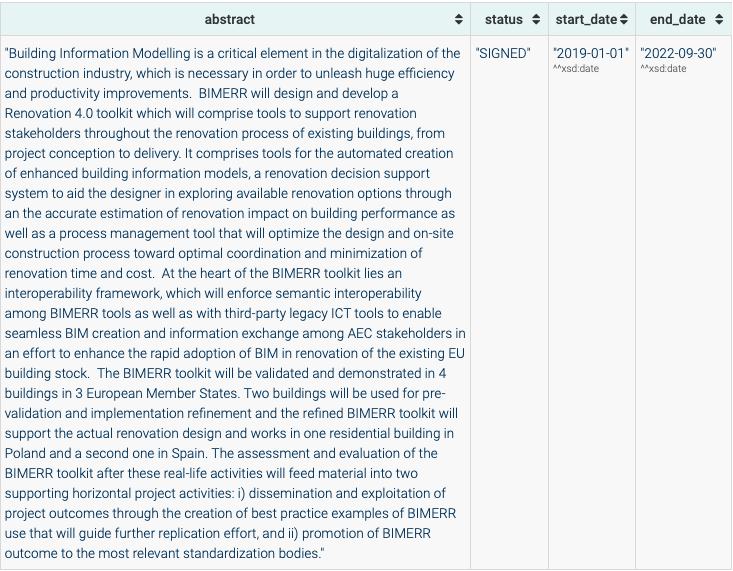
\includegraphics[width=.8\textwidth]{figures/architecture/sparql_example_project1_data_properties.png}
     \rule{35em}{0.5pt}
    \caption{\gls{sparql} query results for getting the abstract, status, start date, and end date of a project titled ``BIM-based holistic tools for Energy-driven Renovation of existing Residences''}
 \label{fig:sparql_example_project1_data_properties}
\end{figure}

We also explored the consortium participants involved in the selected project by querying the \gls{kg} to retrieve the organizations and their roles in the project.
Listing~\ref{lst:sparql_example_project1_consortium_participants} shows the \gls{sparql} query used to extract the consortium participants involved in the project \ref{project1}.
The results of this query are shown in Fig.~\ref{fig:sparql_example_project1_consortium_participants}, providing detailed information about the organizations and their roles in the project.
As we can see, the consortium participants are the same as the ones listed in the scenario analysis in Sec.~\ref{sec:scenarios}.

\begin{lstlisting}[language=SPARQL, caption={\gls{sparql} query for getting the consortium participants involved in a project titled ``BIM-based holistic tools for Energy-driven Renovation of existing Residences''}, label=lst:sparql_example_project1_consortium_participants]
    PREFIX eurio: <http://data.europa.eu/s66#>
    PREFIX rdfs: <http://www.w3.org/2000/01/rdf-schema#>
    SELECT DISTINCT (COALESCE(?org, STRBEFORE(STRAFTER(?party_title, "Org: "), "/ Role:")) AS ?organisation) ?role_label
    WHERE {
        ?project a eurio:Project .
        ?project eurio:title "BIM-based holistic tools for Energy-driven Renovation of existing Residences".
        ?project eurio:title ?project_title.
        ?project eurio:hasInvolvedParty ?party .
        ?party a eurio:OrganisationRole.
        ?party eurio:roleLabel ?role_label.
        ?party rdfs:label ?party_title.
        OPTIONAL { ?party eurio:isRoleOf ?role . ?role rdfs:label ?org. }
    }
\end{lstlisting}

\begin{figure}[htbp]
    \centering
 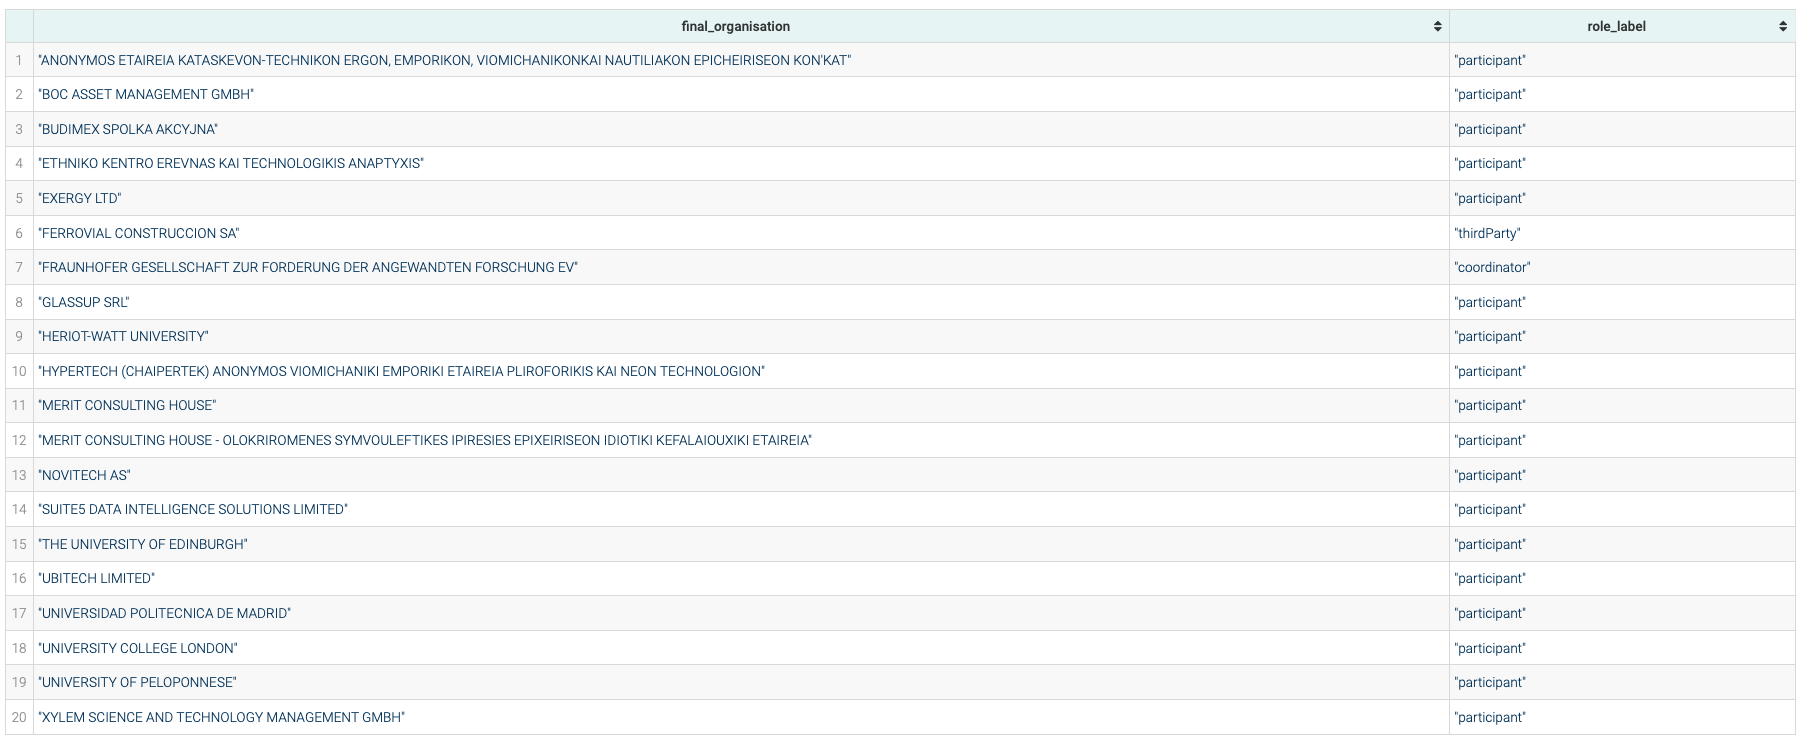
\includegraphics[width=.8\textwidth]{figures/architecture/sparql_example_project1_consortium_participants.png}
     \rule{35em}{0.5pt}
    \caption{\gls{sparql} query results for getting the consortium participants involved in a project titled ``BIM-based holistic tools for Energy-driven Renovation of existing Residences''}
 \label{fig:sparql_example_project1_consortium_participants}
\end{figure}

During the exploration, we also investigated people involved in research projects.
In the \gls{eurio} \gls{kg}, every project includes information about the organizations involved.
Unfortunately, not all projects have the \textit{eurio:isEmployedBy} relationship linking a \textbf{eurio:Role} to a \textbf{eurio:Organisation}.
As a result, it is not always possible to retrieve details about the individuals associated with a given project, since their employment or involvement is not explicitly represented in all cases.
The selected project \ref{project1}, is an example of a project where the people involved are not explicitly linked to the project.
Running the query in Listing~\ref{lst:sparql_example_project1_people} on the \gls{eurio} \gls{kg} did not return any results, indicating that the people involved in the project are not explicitly linked to the project.

\begin{lstlisting}[language=SPARQL, caption={\gls{sparql} query for getting full name, organisation, telephone, and fax of the people involved in a project titled ``BIM-based holistic tools for Energy-driven Renovation of existing Residences''}, label=lst:sparql_example_project1_people]
    PREFIX eurio: <http://data.europa.eu/s66#>
    PREFIX rdfs: <http://www.w3.org/2000/01/rdf-schema#>
    SELECT ?person_label ?org_name ?telephone ?fax
    WHERE {
        ?person a eurio:Person .
        ?person rdfs:label ?person_label .
        ?person eurio:hasContactDetails ?contact_details.
        ?contact_details eurio:telephone ?telephone.
        ?contact_details eurio:faxNumber ?fax.
        ?person eurio:hasRole ?role.
        ?role eurio:isEmployedBy ?org.
        ?org rdfs:label ?org_name.
        ?role eurio:isInvolvedIn ?project.
        ?project a eurio:Project.
        ?project eurio:title "BIM-based holistic tools for Energy-driven Renovation of existing Residences".
    }
\end{lstlisting}

Listing~\ref{lst:sparql_example_merelli_project_people} is the same query as Listing~\ref{lst:sparql_example_project1_people}, but for a different project titled ``Topology driven methods for complex systems''.
The results of this query are shown in Fig.~\ref{fig:sparql_example_merelli_project_people}, providing detailed information about the people involved in the project, including their full name, organization, telephone, and fax.

\begin{lstlisting}[language=SPARQL, caption={\gls{sparql} query for getting full name, organisation, telephone, and fax of the people involved in a project titled ``Topology driven methods for complex systems''}, label=lst:sparql_example_merelli_project_people]
    PREFIX eurio: <http://data.europa.eu/s66#>
    PREFIX rdfs: <http://www.w3.org/2000/01/rdf-schema#>
    SELECT ?person_label ?org_name ?telephone ?fax
    WHERE {
        ?person a eurio:Person .
        ?person rdfs:label ?person_label .
        ?person eurio:hasContactDetails ?contact_details.
        ?contact_details eurio:telephone ?telephone.
        ?contact_details eurio:faxNumber ?fax.
        ?person eurio:hasRole ?role.
        ?role eurio:isEmployedBy ?org.
        ?org rdfs:label ?org_name.
        ?role eurio:isInvolvedIn ?project.
        ?project a eurio:Project.
        ?project eurio:title "Topology driven methods for complex systems".}
\end{lstlisting}

\begin{figure}[htbp]
    \centering
 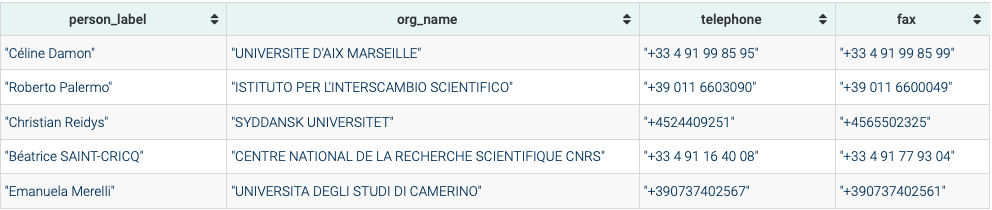
\includegraphics[width=.9\textwidth]{figures/architecture/sparql_example_merelli_project_people.png}
     \rule{35em}{0.5pt}
    \caption{\gls{sparql} query results for getting full name, organisation, telephone, and fax of the people involved in a project titled ``Topology driven methods for complex systems''}
 \label{fig:sparql_example_merelli_project_people}
\end{figure}

The last person in the results of the query in Listing~\ref{lst:sparql_example_merelli_project_people} is Prof. Emanuela Merelli, who is affiliated with the University of Camerino, and Fig.~\ref{fig:example-person-prof-merelli} presents a visual representation of the \gls{eurio} \gls{kg}, specifically focusing on her class type as a \textbf{eurio:Person}.

At the center of the graph, her node connects to multiple entities representing affiliations, roles, projects, and contact details.
The right panel provides metadata about her, including her given name, family name, research control number, and honorific title, indicating her academic status as ``Prof.''.
From Emanuela Merelli's node, one connection leads to a contact details node, which contains her telephone number (+390737402567) and fax number (+390737402561), establishing the \textit{eurio:hasContactDetails} relationship.

\begin{figure}[htbp]
    \centering
 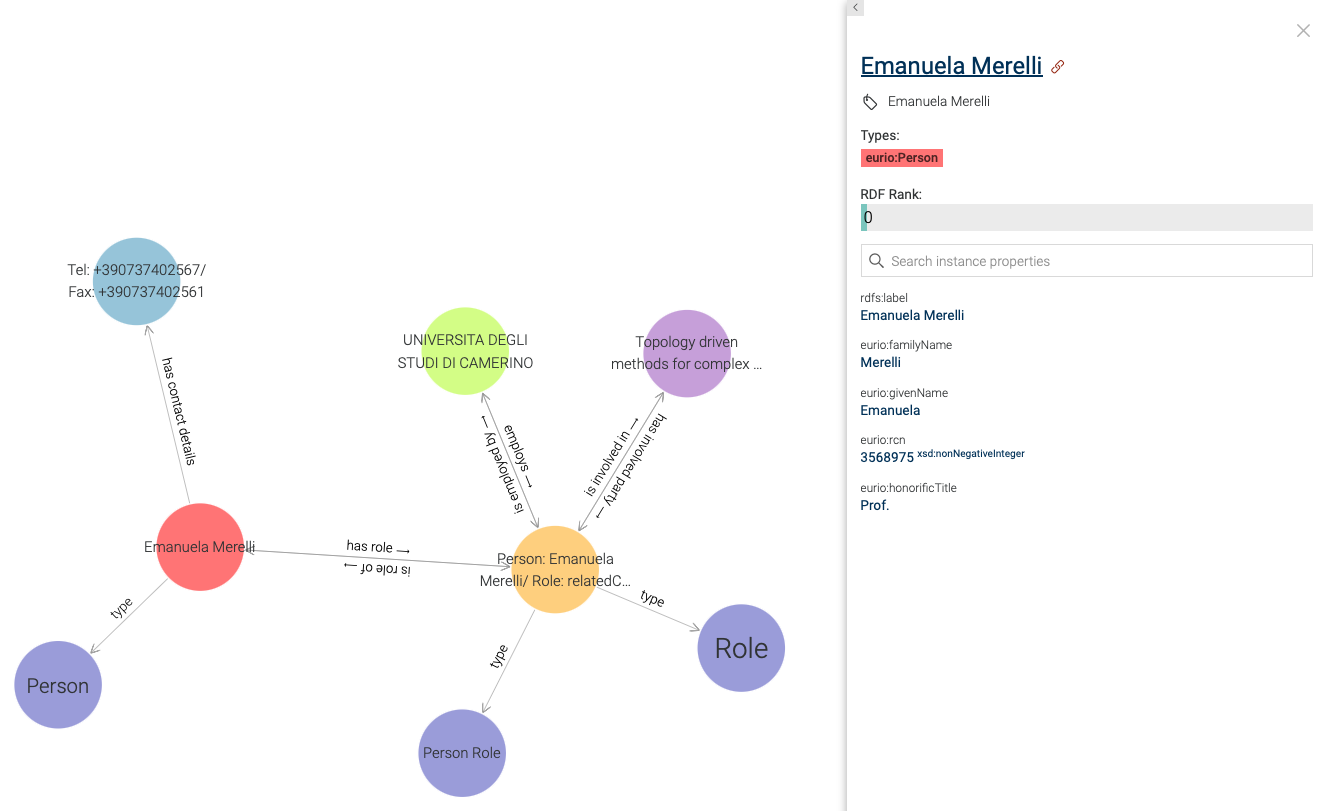
\includegraphics[width=.9\textwidth]{figures/architecture/example-person-prof-merelli.png}
     \rule{35em}{0.5pt}
    \caption{An example of a person's profile in the \gls{eurio} \gls{kg}}
 \label{fig:example-person-prof-merelli}
\end{figure}

Another key connection links her to the ``Universit\`a degli Studi di Camerino'', represented as a green node, with the \textit{eurio:isEmployedBy} relationship, signifying her affiliation with this institution.
Her professional involvement is further detailed through an orange node representing her role, which is bidirectionally linked to her node through the \textit{eurio:hasRole} and \textit{eurio:isRoleOf} relationships.
This \textbf{eurio:PersonRole} node serves as an intermediary between her and the projects she is involved in.
Another significant connection in the graph extends from the role node to a purple node, which is an instance of \textbf{eurio:Project} class, and represents a research project titled ``Topology driven methods for complex systems'', indicating her involvement.
The connection between the role and the project is represented by the \textit{eurio:isInvolvedIn} relationship, confirming her participation in the research activity.
Additional purple nodes represent the classification of roles, distinguishing between general role types and specific person roles.


Through this query-based investigation, we were able to extract detailed information on how projects are interconnected, how participants are structured, and how different elements contribute to the overall knowledge representation within \gls{eurio}.
This \gls{kg} exploration provided a comprehensive understanding of the dataset's richness and limitations, enabling a more informed approach in leveraging the \gls{kg} for our study.

Leveraging the \gls{eurio} ontology, we can effectively address the first sub-research question by structuring and representing data on researchers and research projects within a \gls{kg}.

\section{Recommendation Strategy}\label{sec:recommendation-strategy}


The recommendation strategy in this study was designed to leverage the structured data and relationships within the \gls{eurio} \gls{kg} to generate meaningful and context-aware recommendations.
Given the rich metadata and interconnected entities in \gls{eurio}, we exploited its data properties and relationships to extract the most relevant information about researchers, organizations, and projects.
To facilitate the efficient retrieval of information, we developed a mechanism to query and extract the most meaningful and useful relationships for our purposes, enabling the identification of essential project details, such as the participants in a project, a person's employing organisation, and the organisation's role in a project.
Other useful information to be retrieved is the abstract, duration, status, and url of a project given its title.


\subsection*{Types of Recommendations}
Based on this structured data retrieval, we designed the two following primary types of recommendations.
By integrating these structured recommendations, this strategy enhances the discoverability of research partnerships and collaboration opportunities, leveraging the semantic richness of the \gls{eurio} \gls{kg} to provide personalized and explainable suggestions. The approach ensures that both individual researchers and research organizations receive tailored recommendations based on contextual relevance and domain-specific alignment, making the system an effective tool for fostering research collaboration.

\subsubsection*{Research Collaborator Recommendations}
The first approach focuses on recommending potential research collaborators based on a given project description and its objectives.
By analysing the key attributes of a project, including the title, description and research objectives, the system identifies researchers with expertise in similar fields, ensuring that recommended collaborators are in line with the project's needs, and that they can contribute through their expertise in one or more specific areas, useful for achieving the project's objectives.
In this type of recommendation, it is also useful to refer to projects similar to the one given as input, in which the suggested individual has been involved.

\subsubsection*{Research Consortium Recommendations}
The second approach aims to suggest potential organizations suitable for forming a research consortium, given a project description and objectives.
This recommendation process considers organizational expertise, prior involvement in similar research initiatives, and institutional capabilities, ensuring that the suggested consortium members complement the project's goals.
This type of recommendation is similar to the first one, but here unlike suggesting a list of researchers who are suitable to collaborate on the project, one or more consortia are suggested.
A suggested consortium consists of a group of organisations, which, on the basis of their past participation in other projects, have experience and expertise in achieving one or more of the project objectives.

\section{Architecture Design}\label{sec:architecture-design}
In the suggestion phase, we addressed the second sub-research question:
\begin{center}
    \rqTwo
\end{center}

The proposed system architecture is designed to generate recommendations regarding potential research collaborators for research projects.
Based on the literature requirements (Sec.~\ref{sec:literature-requirements}) and the application requirements (Sec.~\ref{sec:application-requirements}) derived in the problem awareness phase, the defined architecture and the approach we use allow us to fulfil these requirements.
Table~\ref{tab:requirements-fulfillment} shows the list of literature and application requirements and their corresponding fulfillment description.
The fulfilment explanation of each requirement is given later in the description of the proposed architecture.

\begin{table}[htbp]
    \centering
    \scriptsize
    \begin{tabularx}{\textwidth}{|>{\centering\arraybackslash}p{3.5cm}|X|}
      \hline
      \textbf{Literature/Application Requirement} & \textbf{Fulfillment Description}\\
        \hline
        \gls{lr}1 & The \gls{eurio} ontology encodes and provides structured, machine-readable data on EU-funded research projects\\
        \gls{lr}2 &  Similarity search and cosine similarity used as \gls{cbf} recommendation\\
        \gls{lr}3 & \glspl{kg} and \glspl{llm} integration in a \gls{rag} pipeline, combining Graph\gls{rag} and Agentic\gls{rag} to recommend research collaborators without re-training \\
        \gls{lr}4 &  Tool use and multi-agent collaboration patterns used to get retrieval of information and generate recommendations\\
        \gls{appr}1, \gls{appr}2 &  \gls{eurio} \gls{kg} provides a structured and semantically rich representation of EU-funded research projects \\
        \gls{appr}3 & Search web tool used to enrich missing information within the \gls{eurio} \gls{kg}, such as a researcher's areas of interest\\
        \gls{appr}4, \gls{appr}6 &  \gls{eurio} \gls{kg} provides a structured and semantically rich representation of EU organisations \\
        \gls{appr}5, \gls{appr}7 &  \gls{eurio} \gls{kg} provides a structured and semantically rich representation of EU participants \\
        \hline
    \end{tabularx}
    \caption{List of Literature and Application Requirements and their corresponding fulfillment description}
    \label{tab:requirements-fulfillment}
\end{table}


The proposed architecture integrates \glspl{kg} and \glspl{llm} in a \gls{rag} pipeline, following and combining the Graph\gls{rag} and Agentic\gls{rag} paradigms together.
This facilitates the recommendation of potential research collaborators without re-training the model (satisfied \gls{lr}3).
The architecture is built upon the \gls{eurio} \gls{kg}, which provides a structured and semantically rich representation of (EU-funded) research projects (satisfied \gls{appr}1, \gls{appr}2), organizations (satisfied \gls{appr}4, \gls{appr}6), and participants (satisfied \gls{appr}5, \gls{appr}7).
The \gls{eurio} ontology, as described in Sec.~\ref{sec:ontology-selection}, was found as a data model that conceptualizes, formally encodes, and makes available in an open, structured, and machine-readable format data about research projects funded by the EU's framework programmes for research and innovation (satisfied \gls{lr}1).
As shown in Fig.~\ref{fig:proposed-system-graphRAG}, the architecture consists of three main components: the Retrieval Component (red box), the Augmentation Component (purple box), and the Generation Component (blue box).
Before describing each component, we provide a brief overview of the system's user interface, the graph database, the embedding model and vector database, used in the architecture.

\begin{figure}[htbp]
    \centering
 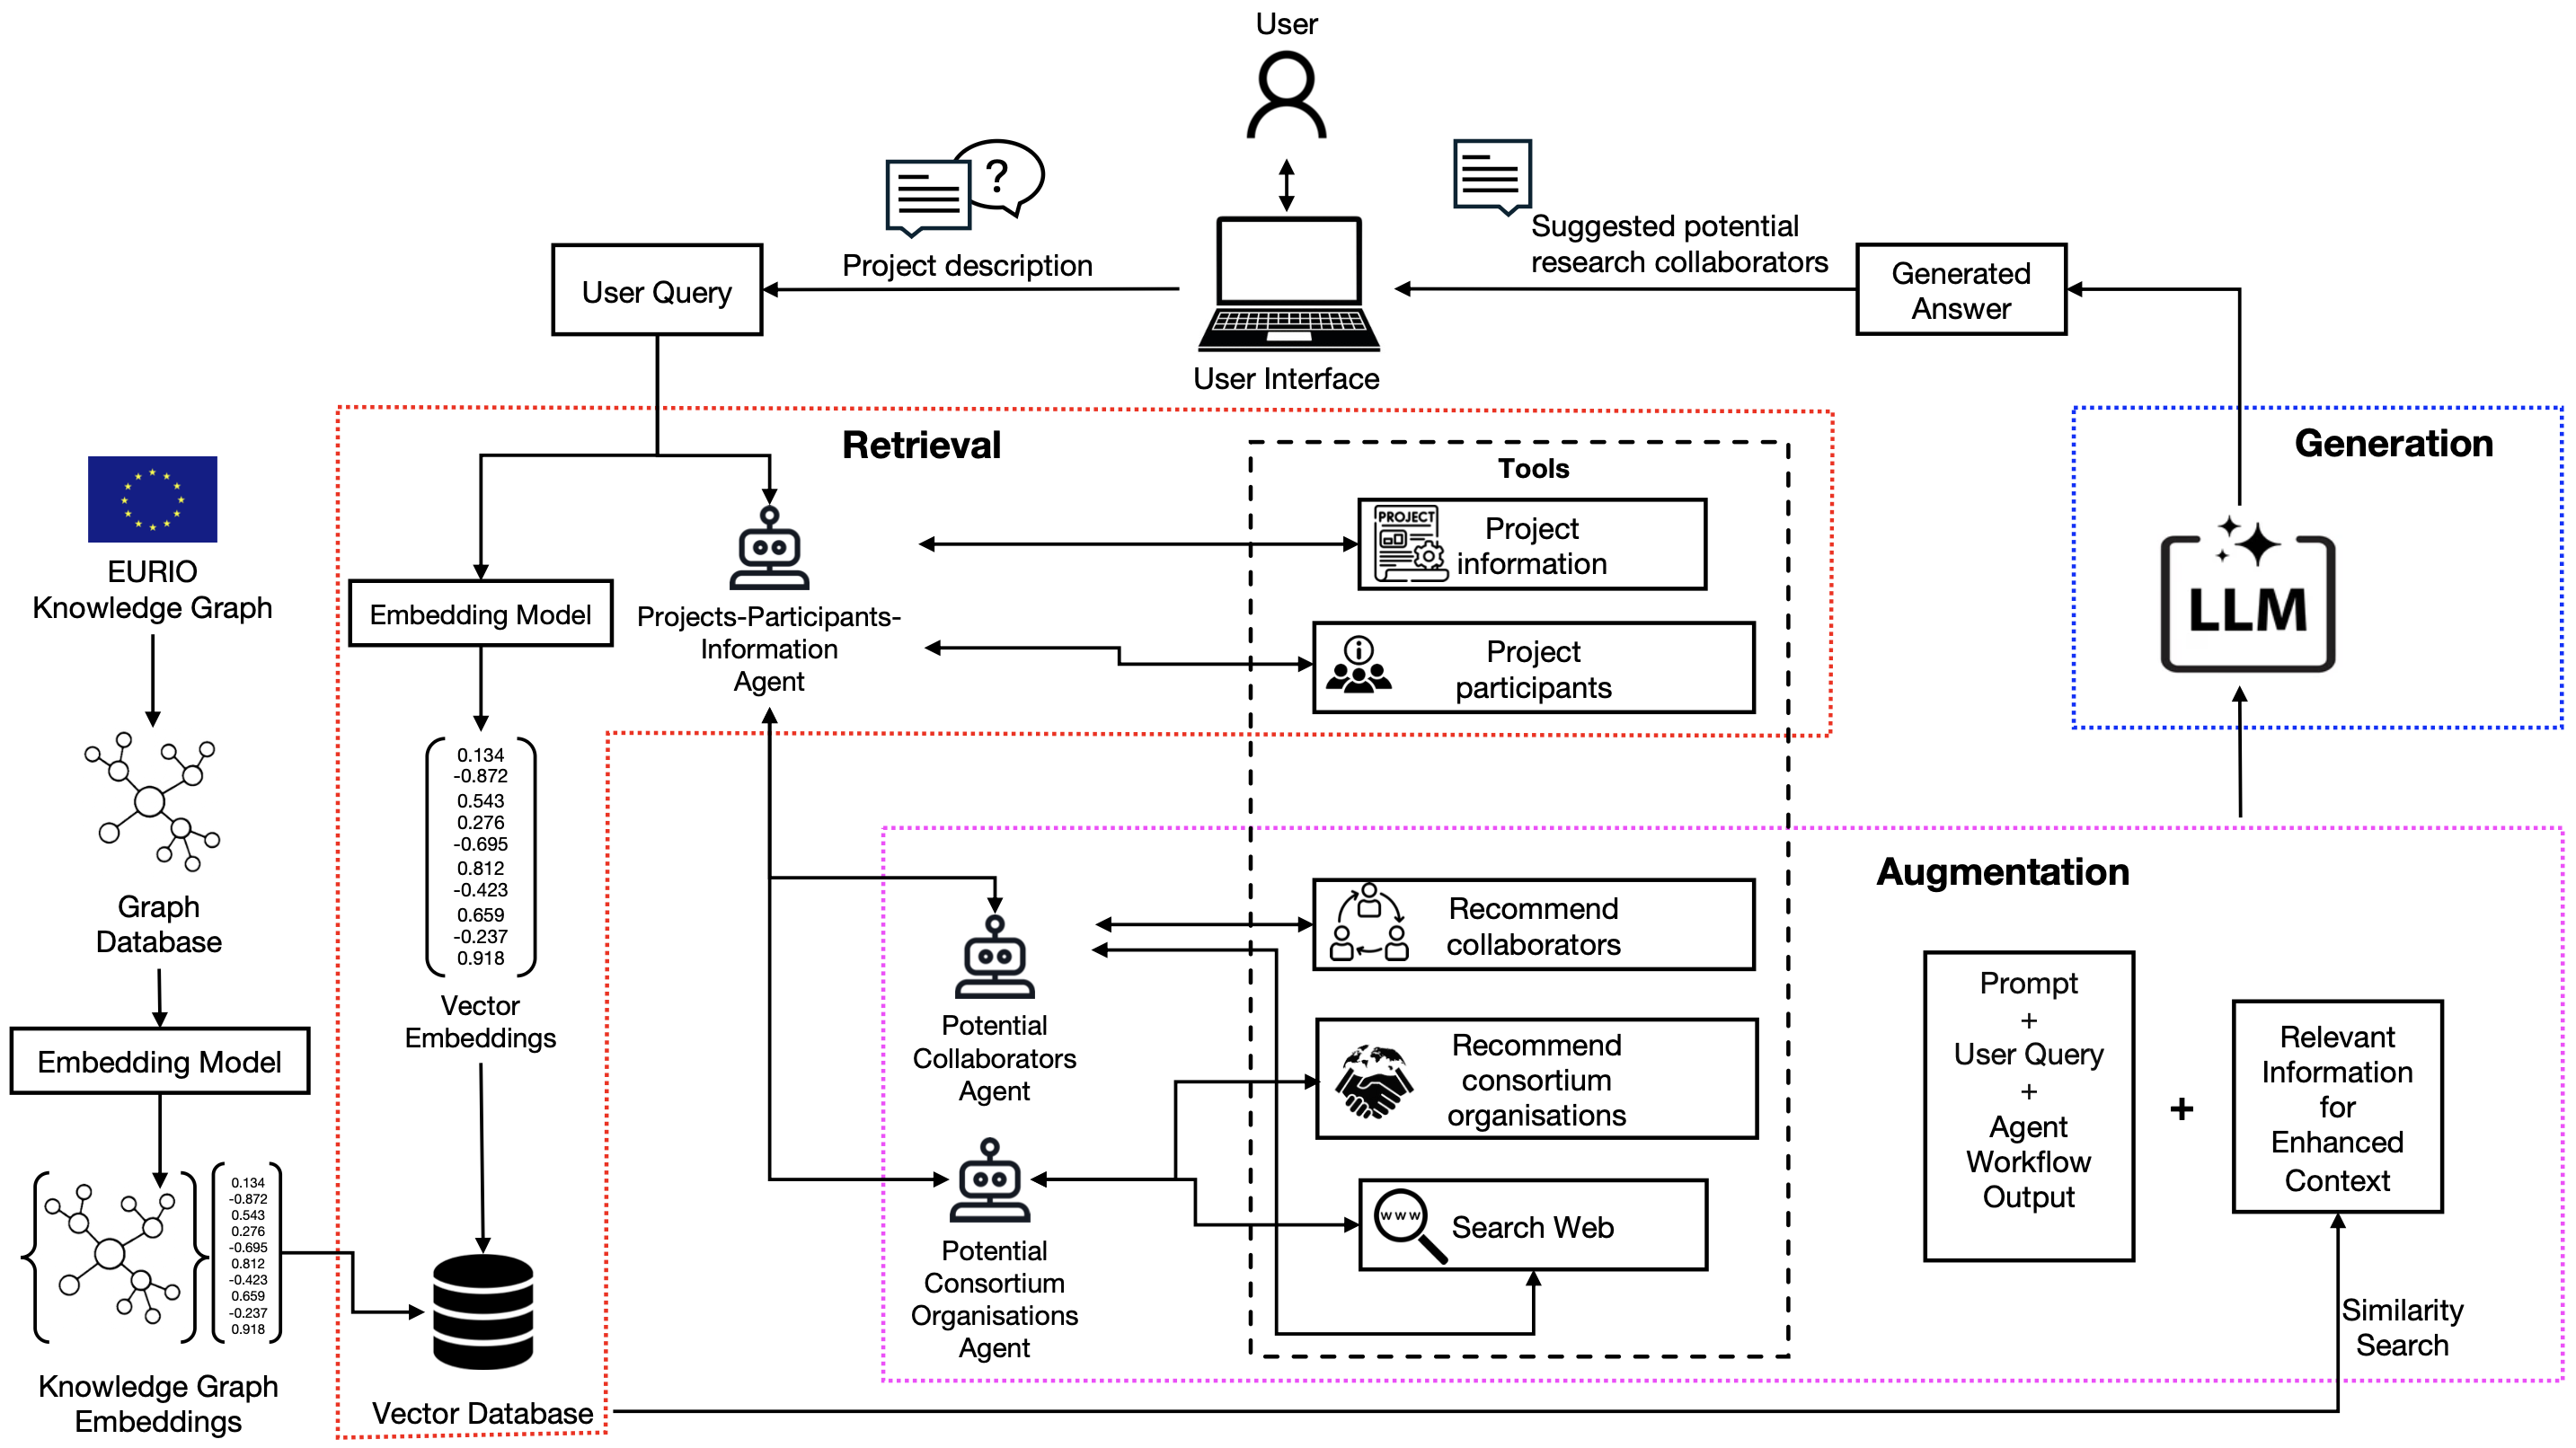
\includegraphics[width=.9\textwidth]{figures/architecture/proposed-system-graphRAG.png}
     \rule{35em}{0.5pt}
    \caption{The proposed Knowledge-Driven and Hybrid AI Architecture for Research Collaboration}
 \label{fig:proposed-system-graphRAG}
\end{figure}

\subsection*{User Interface}
The user interface of the system is designed as a chatbot to provide a user-friendly experience for researchers.
The chatbot provides information retrieval and the two types of recommendations illustrated in Sec.~\ref{sec:recommendation-strategy}.
The user can request information on people, projects and organisation details etc. in the context of European research projects.
It allows users to input a project description and objectives, and receive recommendations for potential research collaborators and consortia.
The interface is designed to be intuitive and easy to use, with clear instructions and guidance on how to input the required information.
The recommendations are displayed in a clear and structured format, with detailed information about each recommended collaborator or consortium, including their expertise, experience, and relevance to the project.

\subsection*{Graph Database}
The \gls{eurio} \gls{kg} is stored as \gls{rdf} format in a graph database, which provides a flexible and efficient way to represent and query the complex relationships between entities in the system.
The graph database allows for the storage of structured data about research projects, organizations, and participants, and enables the retrieval of relevant information based on the relationships between these entities.

\subsection*{Embedding Model and Vector Database}
The embedding model and the vector database play a crucial role in the retrieval process of the proposed system.
\gls{eurio}'s \gls{kg}, stored in a graph database, is transformed through an embedding model, which converts structured information into numerical vector representations.
These embeddings capture the semantic relationships between entities in the \gls{kg}, enabling efficient similarity searches.
The generated vector embeddings are stored in a vector database, facilitating rapid retrieval of relevant knowledge.
When a user submits a query, it is also converted into an embedding and compared against the stored vectors in a similarity search to identify relevant projects, participants, or research entities (satisfied \gls{lr}2).

\subsection*{Agentic Graph Retrieval-Augmented Generation}
Our approach combines the Graph\gls{rag} and Agentic\gls{rag} paradigms to create a hybrid \gls{ai} architecture that leverages the structured data in the \gls{eurio} \gls{kg} and the vector database to generate contextually accurate and consistent recommendations.
According to \cite{singh2025}, modern agents, such as \gls{llm}-powered and mobile agents, are intelligent entities that can perceive their environment, reason about it, and autonomously perform tasks.
In our architecture, 3 agents were defined: the \textit{Project-Participants-Information Agent}, the \textit{Project-Organization-Information Agent}, and the \textit{Project-Researcher-Information Agent}.
These agents follow two agentic workflow patterns \cite{singh2025}: the tool use pattern and the multi-agent collaboration pattern (satisfied \gls{lr}4).
As explained in the following paragraphs, the proposed architecture consists of three main components: Retrieval, Augmentation, and Generation, and agents work together within these components, using external tools to expand their capabilities to achieve specific goals.
A detailed description of each agent using its own tools is given in Sec~\ref{sec:building-ai-agents}.

\paragraph*{Retrieval Component.}
This component is responsible for retrieving relevant information from the \gls{eurio} \gls{kg} and the vector database.
The agent workflow is always initiated by the master agent: the \textit{Project-Participants-Information Agent}.
This agent is responsible for returning information about projects, such as the (e.g. project abstract), and also for returning information about the participants involved in that project (e.g. person full name, organization details).
To perform the retrieval of this information, the agent was specified to follow a template prompt, in which it is instructed to generate \gls{sparql} queries to query the \gls{eurio} \gls{kg} from which to extract data.
Depending on the task to be performed, the master agent will delegate that task to the agent responsible for that task, if necessary.

\paragraph*{Augmentation Component.}
In addition to combining the user query, prompt templates, and information retrieved from the agent master, with all relevant information obtained from the similarity search (satisfied \gls{lr}2), this component adds additional data from the activity performed by the agent workflow.
Cosine similarity was used as a metric for semantic search to determine the similarity of embeddings.
In this component, the agents \textit{Potential Collaborators Agent} and \textit{Potential Consortium Organisations Agent} are responsible for creating the recommendations.
The \textit{Potential Collaborators Agent} has the task of recommending research collaborators, given a project description as input.
The \textit{Potential Consortium Organisations Agent} has the task of creating several consortia formed by various organisations, which contribute to the consortium in a complementary way, i.e. there will be no consortia with organisations specialising in the same research area.
These two agents use the \textit{recommend collaborators} tool, and the \textit{Recommend consortium organisations} tool, respectively, to accomplish the tasks previously described, and they too are instructed with specific prompt templates to follow to achieve their goal.
In addition, both use the \textit{search web} tool, to enrich the information obtained, such as a researcher's areas of interest (satisfied \gls{appr}3), which are not present within the \gls{eurio} \gls{kg}.
In this way, agents act autonomously and are able to make dynamic decisions, resulting in better results than a graph.

\paragraph*{Generation Component.}
Finally, the generation component combines all previously retrieved and augmented information with the pre-trained knowledge of the \gls{llm} to generate contextually accurate and consistent responses.
In addition to providing relevant recommendations, this component ensures explainability by offering detailed justifications for suggested research collaborators, outlining the reasons behind their selection based on expertise, involvement in previous projects and research alignment.
It also describes how the proposed research consortia are composed, specifying the complementary roles of the participating organisations and their collective ability to achieve the project objectives.
This increases transparency and trust in the recommendation process, making the system a valuable tool for making informed decisions in research collaborations.
\fillingPage{}
\chapter{A Research Collaboration Recommender Based on Hybrid AI}\label{chap:ArtifactDevelopment}

This chapter presents the implementation of the proposed Knowledge-Driven and Hybrid \gls{ai} Architecture for Research Collaboration.
First of all, the technology stack used in the proposed system is described in Sec.~\ref{sec:technology-stack}.
Then, the process of populating the databases is explained in Sec.~\ref{sec:databases-population}.
Finally, the section \ref{sec:building-ai-agents} describes in detail the development of the agents and tools \gls{ai}, providing several examples of system use for each agent.

In the implementation phase, we addressed the third sub-research question:
\begin{center}
    \rqThree
\end{center}

\section{Technology Stack}\label{sec:technology-stack}
The proposed system is built entirely in \texttt{Python}, using \texttt{Streamlit} for both the back-end and front-end to simplify web app development and sharing.
\texttt{GraphDB}, developed by Ontotext, was chosen as the graph database for our system because of its robust support for the \gls{rdf} standard, enabling semantic data representation, efficient \gls{sparql} querying, and easy integration with \glspl{kg} for enhanced reasoning and retrieval.
Additionally, \texttt{Chroma} was selected as the vector database for storing \gls{kg} embeddings due to its efficient similarity search, scalable storage, and suitable integration with machine learning pipelines, ensuring fast and accurate retrieval of relevant entities.
To compute embeddings, we selected the \texttt{all-MiniLM-L6-v2} model due to its efficiency and strong performance in semantic similarity tasks.
This model is particularly well-suited for encoding short to medium-length text, making it ideal for our use case, where we store and retrieve project titles and abstracts from the \gls{eurio} dataset.
By leveraging a lightweight transformer architecture, \texttt{all-MiniLM-L6-v2} balances accuracy and computational efficiency, enabling fast and effective similarity search within our system.
To run the \texttt{all-MiniLM-L6-v2} model, we utilized \texttt{Ollama}, a lightweight, extensible framework for building and running language models on the local machine.
To implement our Graph\gls{rag} and Agentic\gls{rag} approach, we utilized two main frameworks: \texttt{LlamaIndex} was employed to build the agent workflow, coordinate agents, and integrate tools, while \texttt{LangChain} primarily facilitated the generation of \gls{sparql} queries from user query inputs.
For response generation, we utilized one of the state-of-the-art \glspl{llm}: \texttt{GPT-4o}, developed by OpenAI.
The context window and maximum output tokens for this model are detailed in Table~\ref{table:gpt-4o-tokens}, which illustrates its suitability for handling long input queries and generating high-quality responses.
The token limit represents the maximum number of tokens a model can handle in a single input, where a token typically corresponds to approximately \textsuperscript{3}/\textsubscript{4} of a word or four characters.

\begin{table}[htbp]
    \centering
    \begin{tabularx}{\textwidth}{|X|X|X|}
      \hline
      \textbf{Model} & \textbf{Context Window} & \textbf{Max Output Tokens}\\
      \hline
      GPT-4o 2024-05-13 & 128K tokens & 4,096 tokens\\
      \hline
    \end{tabularx}
    \caption{Context window and token limit of the GPT-4o model}
    \label{table:gpt-4o-tokens}
\end{table}

Finally, we containerized the entire system using \texttt{Docker} to ensure portability, reproducibility, and scalability across different environments.
The technology stack used in the proposed Knowledge-Driven and Hybrid \gls{ai} Architecture for Research Collaboration is summarized in Table~\ref{tab:technology-stack}.
Fig.~\ref{fig:proposed-system-graphRAG-technologies} provides a visual representation of the technologies used in the proposed system.
The source code for the proposed system is available on GitHub at \url{https://github.com/Piermuz7/MasterThesisProject.git}.

\begin{table}[htbp]
    \centering
    \scriptsize
    \begin{tabularx}{\textwidth}{|>{\centering\arraybackslash}p{2cm}|>{\centering\arraybackslash}p{2.5cm}|X|X|}
      \hline
      \textbf{Category} & \textbf{Technology/Tool} & \textbf{Description} & \textbf{Purpose/Usage} \\
        \hline
        Programming Languages & \texttt{Python} & A high-level, general-purpose programming language & Research Colaborator Recommender Development\\
        \hline
        Libraries & \texttt{Streamlit} & An open-source app framework for Machine Learning and Data Science projects & Front-end and back-end development\\
        \hline
        Graph Databases & \texttt{GraphDB} & A family of highly efficient, robust, and scalable \gls{rdf} databases & Knowledge Graph Population\\
        \hline
        Query Languages & \texttt{\gls{sparql}} & A query language and protocol for \gls{rdf} databases & Knowledge Graph Querying\\
        \hline
        Vector Databases & \texttt{Chroma} & An open-source vector database for storing and retrieve embeddings & Knowledge Graph Embeddings Storage\\
        \hline
        Embedding Models & \texttt{all-MiniLM-L6-v2} & A small but powerful model trained to generate high-quality sentence embeddings & Knowledge Graph Embeddings Generation\\
        \hline
        \glspl{llm} & \texttt{GPT-4o} & A multilingual, multimodal generative pre-trained transformer & Answer Generation in the \gls{rag} pipeline\\
        \hline
        Frameworks & \texttt{LangChain} & An open-source framework for developing applications powered by \glspl{llm} & \glspl{sparql} query generation in \gls{rag} pipeline development\\
        \hline
        Frameworks & \texttt{LlamaIndex} & An open source data orchestration framework for building applications based on \glspl{llm} & Agent Workflow in \gls{rag} pipeline development\\
        \hline
        Frameworks & \texttt{Ollama} & A lightweight, extensible framework for building and running language models on the local machine & Used to run all-MiniLM-L6-v2\\
        \hline
        Containerization and Deployment & \texttt{Docker} & An open platform for developing, shipping, and running applications & Containerization of the entire system\\
        \hline
    \end{tabularx}
    \caption{Technology stack used in the proposed Knowledge-Driven and Hybrid \gls{ai} Architecture for Research Collaboration}
    \label{tab:technology-stack}
\end{table}

\begin{figure}[htbp]
    \centering
 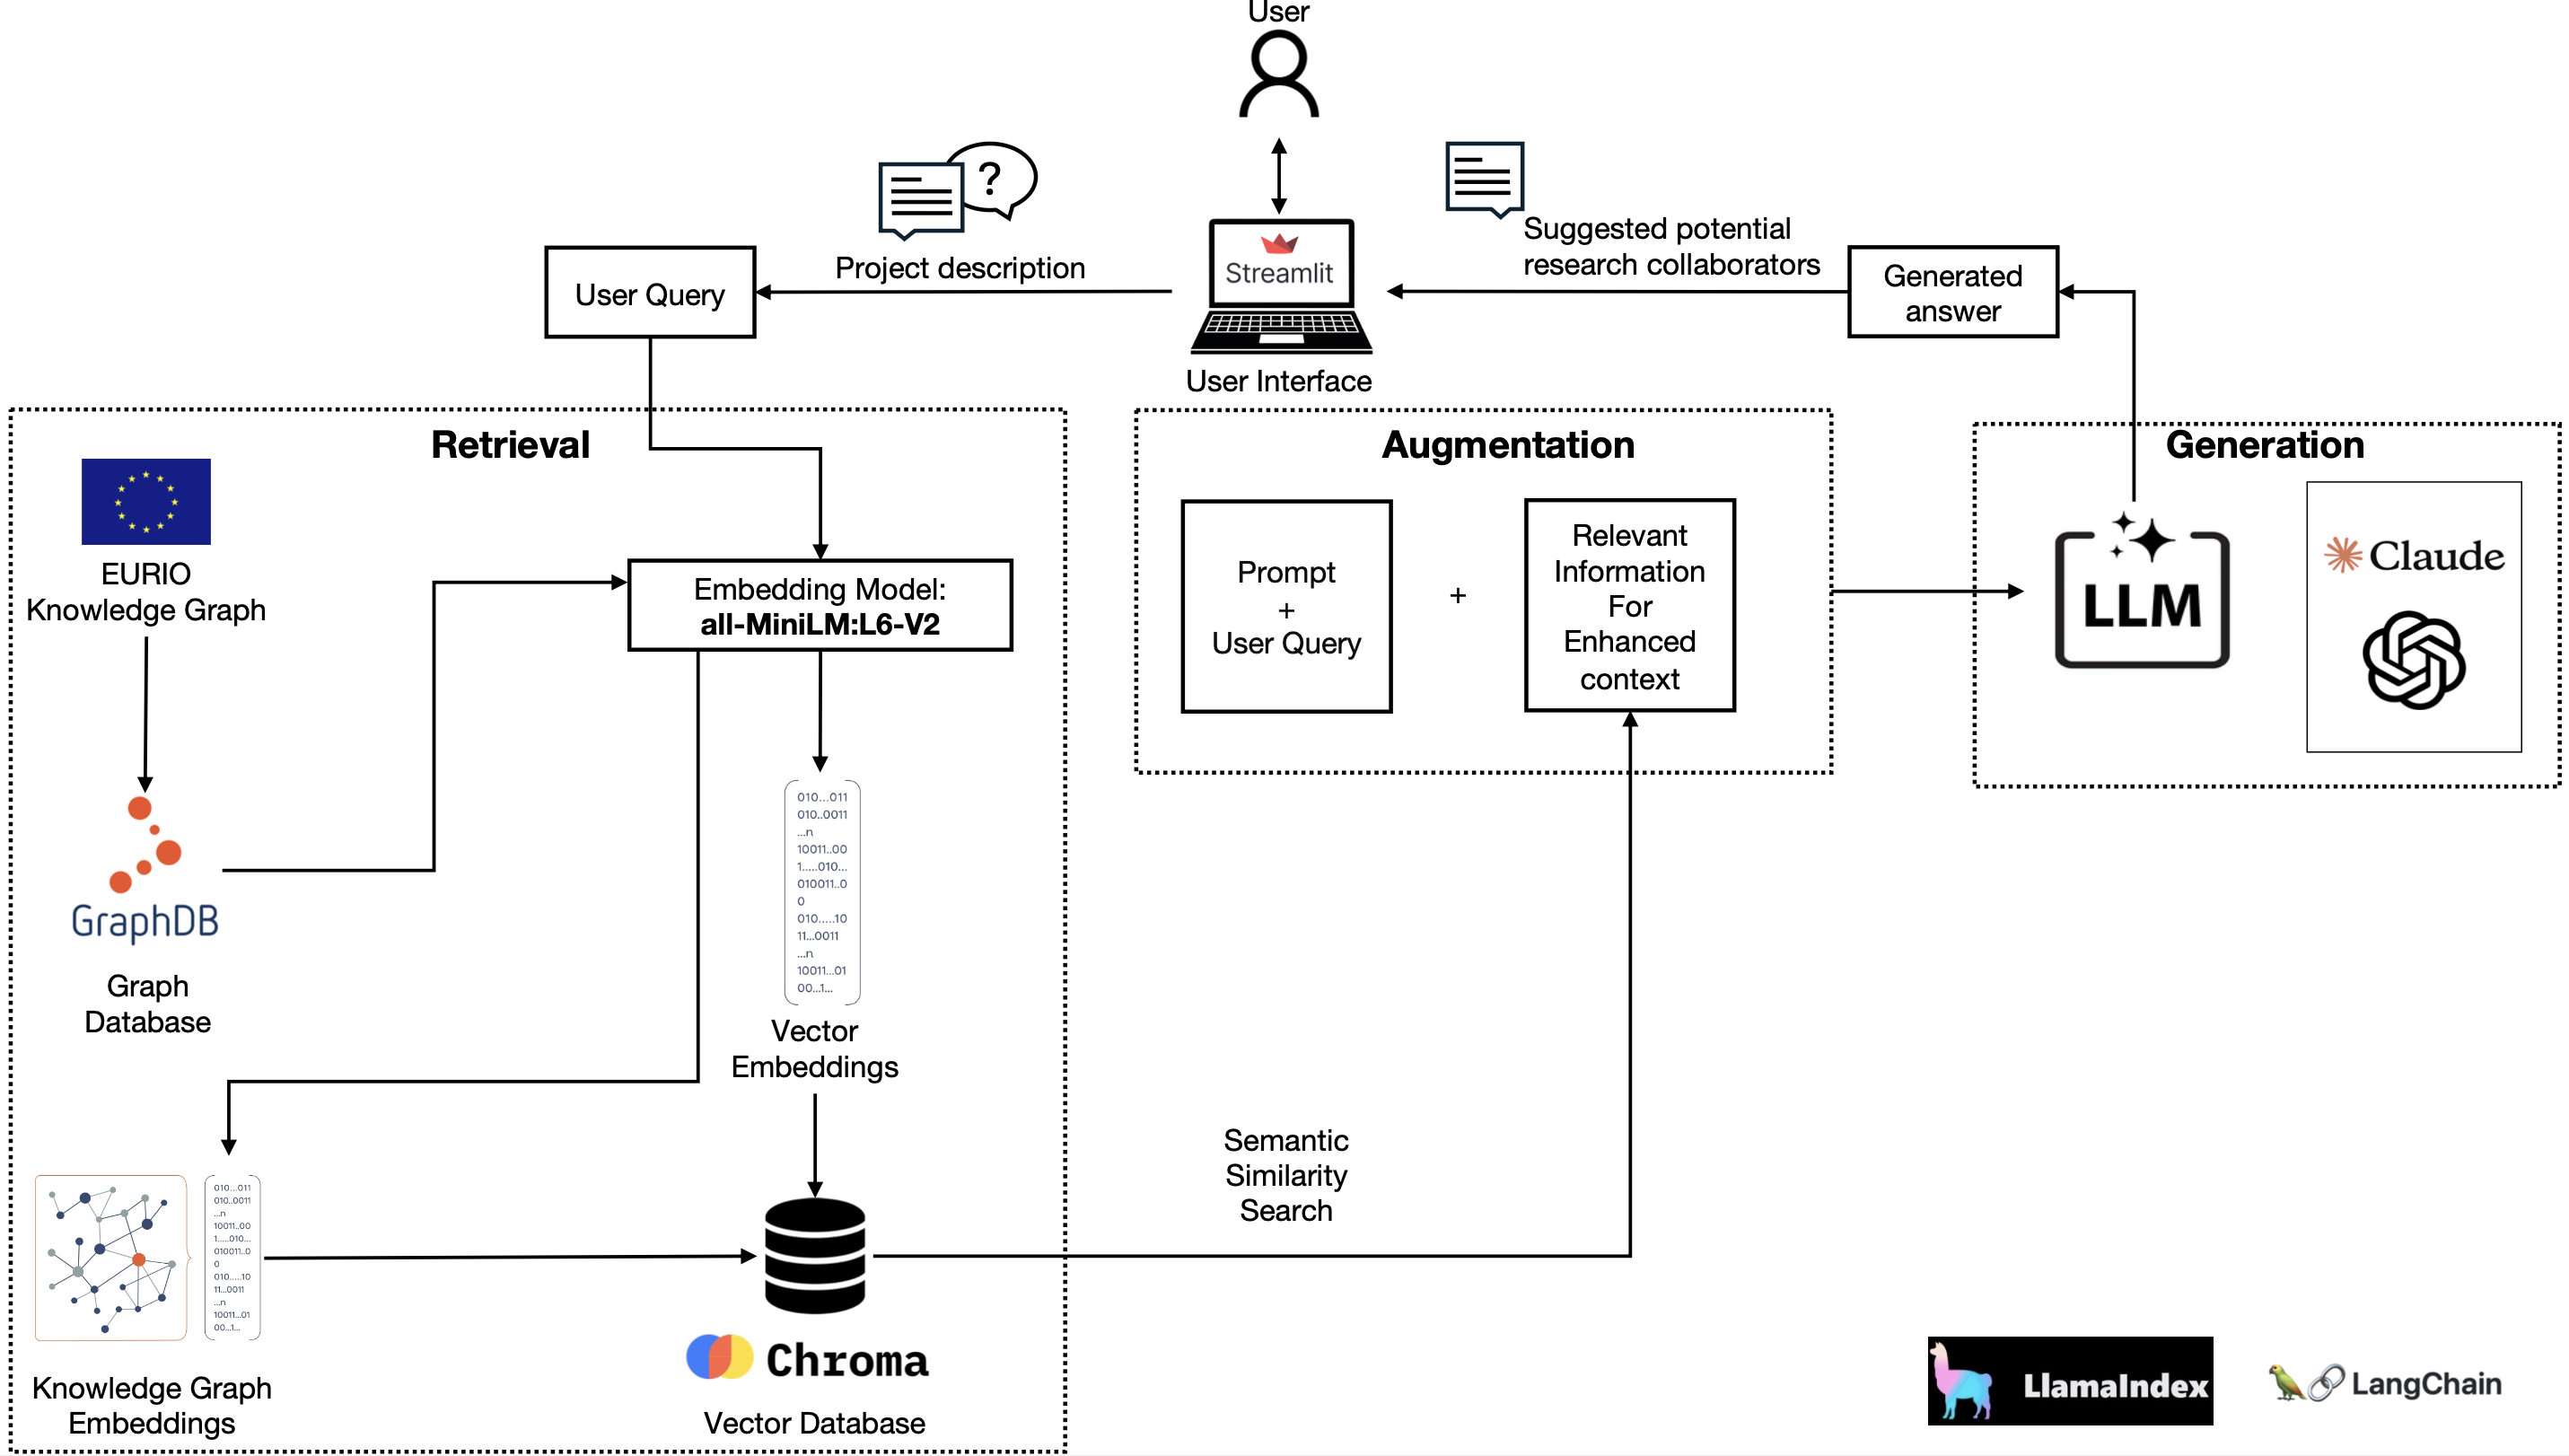
\includegraphics[width=.9\textwidth]{figures/implementation/proposed-system-graphRAG-technologies.png}
     \rule{35em}{0.5pt}
    \caption{Technologies used in the proposed Knowledge-Driven and Hybrid AI Architecture for Research Collaboration}
 \label{fig:proposed-system-graphRAG-technologies}
\end{figure}

\section{Databases Population}\label{sec:databases-population}
The first step is populating the databases, which involves importing the \gls{eurio} \gls{kg}, provided in \gls{rdf} N-Quad format, into GraphDB.
This process ensures that the structured knowledge about EU-funded research projects is stored in a graph database, allowing for efficient querying and retrieval of relevant information.
During the \acrlong{kg} Exploration (Sec.~\ref{sec:ontology-selection}), it was observed that not all projects within the \gls{eurio} dataset have associated participants.
In other words, certain projects exist in the \gls{kg} without any recorded participants.
Given that the goal of the system is to recommend research collaborators based on project involvement, it is crucial to ensure that only relevant data is processed in the embedding generation phase.
To maintain efficiency and relevance, embeddings of title and abstract are computed only for projects that have at least one associated participant.
This is achieved by filtering out projects without participants using the \gls{sparql} query shown in Listing~\ref{lst:projects-with-at-least-one-participants}.

\begin{lstlisting}[language=SPARQL, caption={\gls{sparql} query for getting the projects with at least one participant}, label={lst:projects-with-at-least-one-participants}]
    PREFIX eurio: <http://data.europa.eu/s66#>
    PREFIX rdfs: <http://www.w3.org/2000/01/rdf-schema#>
    SELECT DISTINCT ?project ?title ?abstract
    WHERE {
        ?project a eurio:Project .
        ?project eurio:title ?title .
        ?project eurio:abstract ?abstract .
        FILTER EXISTS {
            ?project eurio:hasInvolvedParty ?party .
            ?party a eurio:OrganisationRole .
            ?party eurio:isRoleOf ?role .
            ?person eurio:isInvolvedIn ?project .
            ?person eurio:isEmployedBy ?role .
            ?person eurio:isRoleOf ?p .
        }
    }
\end{lstlisting}

The query \gls{sparql} returned 25,482 projects with at least one participant involved in each project.
Of these projects, title and abstract embeddings were calculated and stored in the Chroma vector database.
In this way, the vector database contains only meaningful representations of research projects with involved participants, avoiding unnecessary computations for projects without involved participant.
Consequently, no storage space is wasted in the vector database.
Since the \gls{kg} is too large to process in a single step, embedding storage in Chroma was performed in batches.
Specifically, embeddings were stored 1,000 entities at a time to efficiently manage memory usage and avoid performance bottlenecks.

\section{Building AI Agents and Tools}\label{sec:building-ai-agents}
Once the \gls{kg} and related embeddings are stored in the databases, we need to implement the system's core functionalities.
This involves building \gls{ai} agents and tools to facilitate the recommendation process.
As described in Sec.~\ref{sec:architecture-design}, the user interface is designed as a chatbot, where users can interact with the system by asking questions and receiving responses.
To enable this interaction, we developed three main agents and five different tools.
The agents are responsible for coordinating the workflow, generating responses, and managing the system's overall functionality.
The tools, on the other hand, are designed to perform specific tasks, such as generating \gls{sparql} queries, extracting relevant information, and providing recommendations.
Going into technical details, \textbf{LlamaIndex} is used to set a prompt to agents, which instructs agents to execute specific tools, respond according to a certain format, and so on.
\textbf{Langchain}, on the other hand, is used exclusively for generating \gls{sparql} queries based on user input.
The data returned from these queries will then be used in turn by the agents.
The agents and tools are described in more detail below.
For the sake of readability, only the prompt templates of the agents are given in the appendices.
Also for these reasons, the tool names used in this thesis are not the same as those given in the prompt templates in the appendices.


\subsection*{Project-Participants-Information Agent}
The process starts with a user query, which is handled by a coordinator agent, also called master agent.
This agent serves as the central orchestrator, executing a specific task, or assigning the query to specialized retrieval agents according to its specific requirements.
In other words, this agent is tasked with retrieving information on projects and participants.
It is equipped with a template prompt that it must follow.
The prompt, shown in the Appendix~\ref{app:ProjectParticipantsAgent}, sets the scope of the agent, making it explicit that it must answer purely related questions in the context of European projects.
With this prompt, the agent is instructed on how to use its tools: \textit{Project information} and \textit{Project participants}.
The first tool has example \gls{sparql} queries to generate a \gls{sparql} query from the user query.
For example, if the user asks for the relative information of a project entitled ``Knowledge-Based Information Agent with Social Competence and Human Interaction Capabilities'', the agent will use this tool to generate the \gls{sparql} query shown in Listing~\ref{lst:project-information-sparql-query}.

\begin{lstlisting}[language=SPARQL, caption={\gls{sparql} query for getting information of a project entitled ``Knowledge-Based Information Agent with Social Competence and Human Interaction''}, label={lst:project-information-sparql-query}]
PREFIX eurio: <http://data.europa.eu/s66#>
SELECT DISTINCT ?title ?url ?abstract ?status ?startDate ?endDate
WHERE{
    ?project a eurio:Project .
    ?project eurio:title "Knowledge-Based Information Agent with Social Competence and Human Interaction Capabilities" .
    ?project eurio:title ?title .
    ?project eurio:url ?url .
    ?project eurio:abstract ?abstract .
    ?project eurio:projectStatus ?status .
    ?project eurio:startDate ?startDate .
    ?project eurio:endDate ?endDate .
}
\end{lstlisting}

Once, the information is retrieved, the agent will use its prompt template to generate a response with such information.

The second tool also has its own template with SPARQL queries to follow as an example for generating queries to obtain information on participants.
An example query set in the prompt of this tool is shown as follows.
If the user asks ``Who is Emanuela Merelli?'', the agent will use this tool to generate the \gls{sparql} query shown in Listing~\ref{lst:person-information-sparql-query}.
This query retrieves information about a person named Emanuela Merelli, including their organization, contact details, and projects they are involved in.

\begin{lstlisting}[language=SPARQL, caption={\gls{sparql} query for getting information of a person}, label={lst:person-information-sparql-query}]
PREFIX eurio: <http://data.europa.eu/s66#>
PREFIX rdfs: <http://www.w3.org/2000/01/rdf-schema#>
SELECT ?person_label ?org_name ?telephone ?fax ?project_title
WHERE {
    ?person a eurio:Person .
    ?person rdfs:label ?person_label .
    ?person eurio:hasContactDetails ?contact_details .
    ?contact_details eurio:telephone ?telephone .
    OPTIONAL{{?contact_details eurio:faxNumber ?fax .}}
    FILTER (LCASE(?person_label) = "emanuela merelli") .
    ?person eurio:hasRole ?role .
    ?role eurio:isEmployedBy ?org .
    ?org rdfs:label ?org_name .
    ?role eurio:isInvolvedIn ?project .
    ?project a eurio:Project .
    ?project eurio:title ?project_title .
}
\end{lstlisting}

Fig.~\ref{fig:example-who-is-emanuela-merelli} shows an example of a user query asking for information about a person named Emanuela Merelli, using the chatbot interface.

\begin{figure}[htbp]
    \centering
 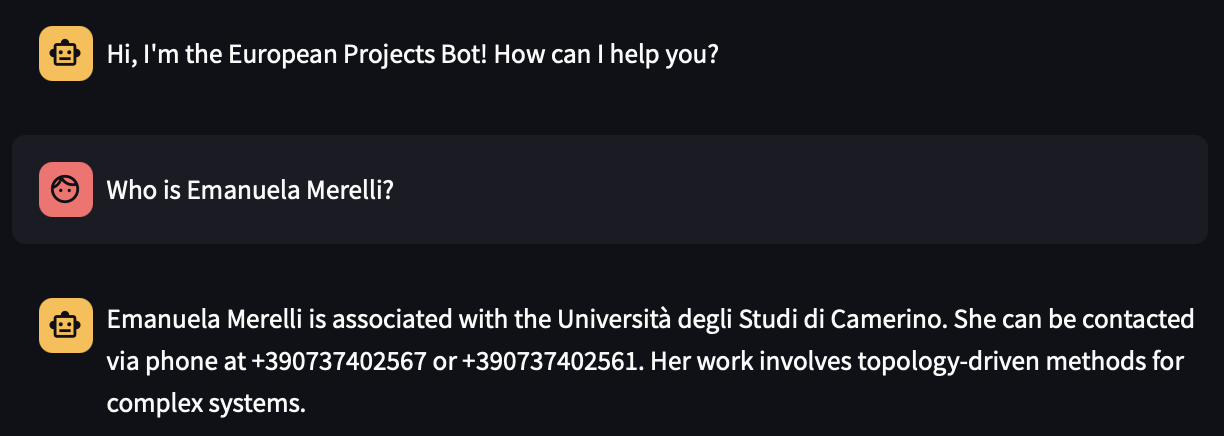
\includegraphics[width=.8\textwidth]{figures/implementation/example-who-is-emanuela-merelli.png}
     \rule{35em}{0.5pt}
    \caption{Example of a user query asking for information about a person named Emanuela Merelli}
 \label{fig:example-who-is-emanuela-merelli}
\end{figure}

Another example of a user query asking for information about a project entitled ``Topology-Driven Methods for Complex Systems'' is shown in Fig.~\ref{fig:example-general-info-about-topology-driven-methods-for-complex-systems-project}.
This query is handled by the same agent, which uses the \textit{Project information} tool to generate the \gls{sparql} query to retrieve the project's metadata.
The chatbot's response presents the abstract of the project and briefly explains which topics it focused on and the types of scientists involved.
However, it does not mention the researchers involved, because the \textit{Participant information} tool was not used.
Finally, the duration and two useful links related to the project are given.

\begin{figure}[htbp]
    \centering
 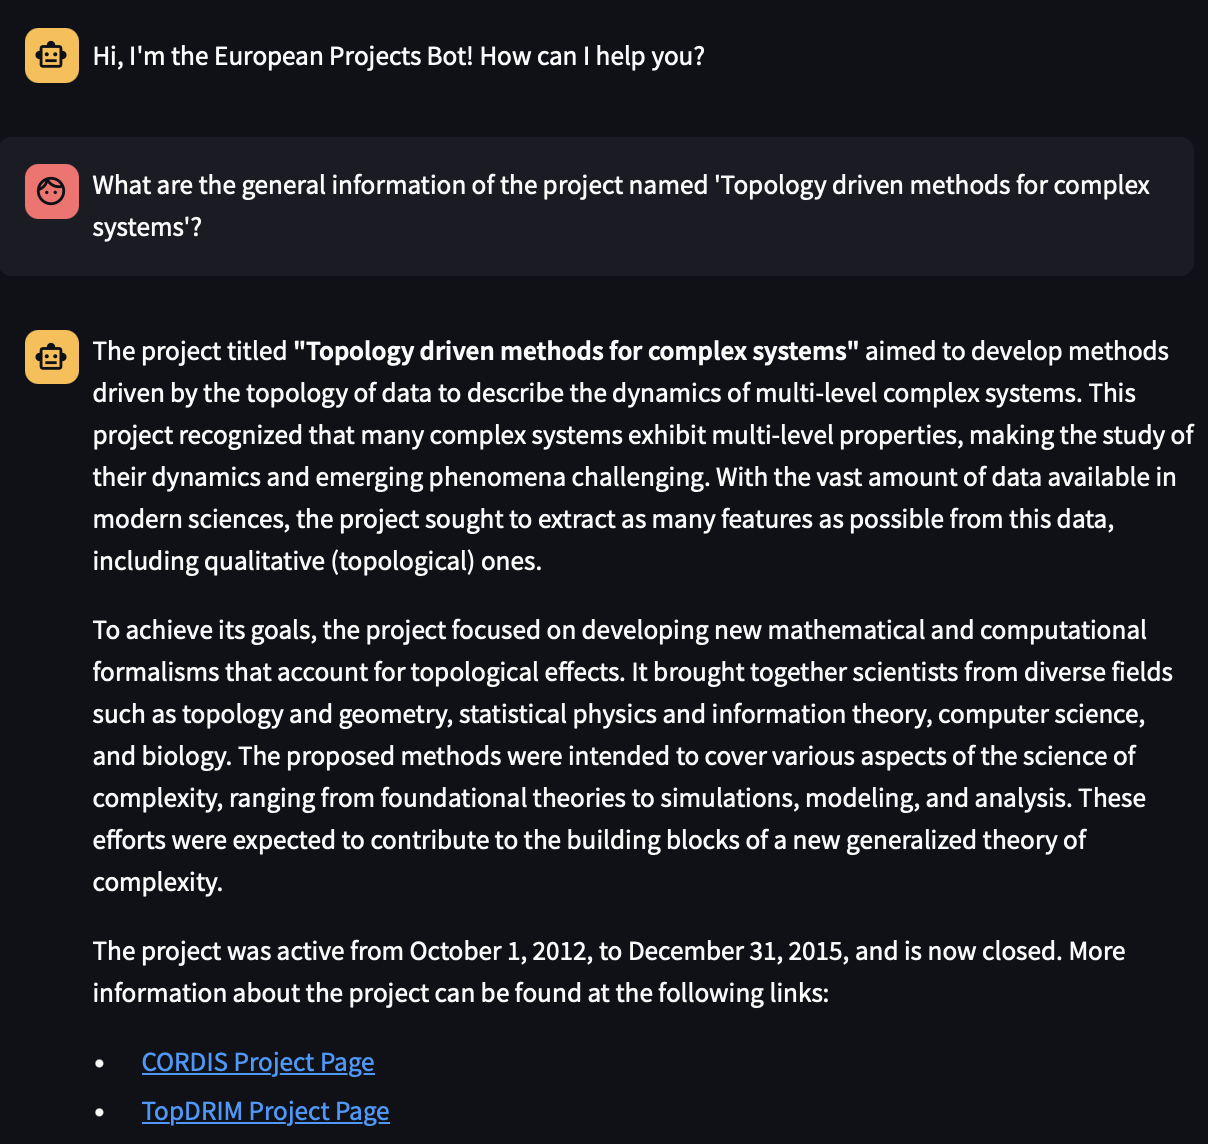
\includegraphics[width=.8\textwidth]{figures/implementation/example-general-info-about-topology-driven-methods-for-complex-systems-project.png}
     \rule{35em}{0.5pt}
    \caption{Example of a user query asking for information about a project entitled ``Topology-Driven Methods for Complex Systems''}
 \label{fig:example-general-info-about-topology-driven-methods-for-complex-systems-project}
\end{figure}

Fig.~\ref{fig:example-participants-of-topology-driven-methods-for-complex-systems-project} shows an example of a user query asking for information about participants in the same project.
This query is handled by the same agent, which uses the \textit{Project participants} tool to generate the \gls{sparql} query to retrieve the project's participants.
In this example, the project coordinator and the 5 participants involved are listed.
In addition, the organisation and its postal address where this participant is employed is given.

\begin{figure}[htbp]
    \centering
 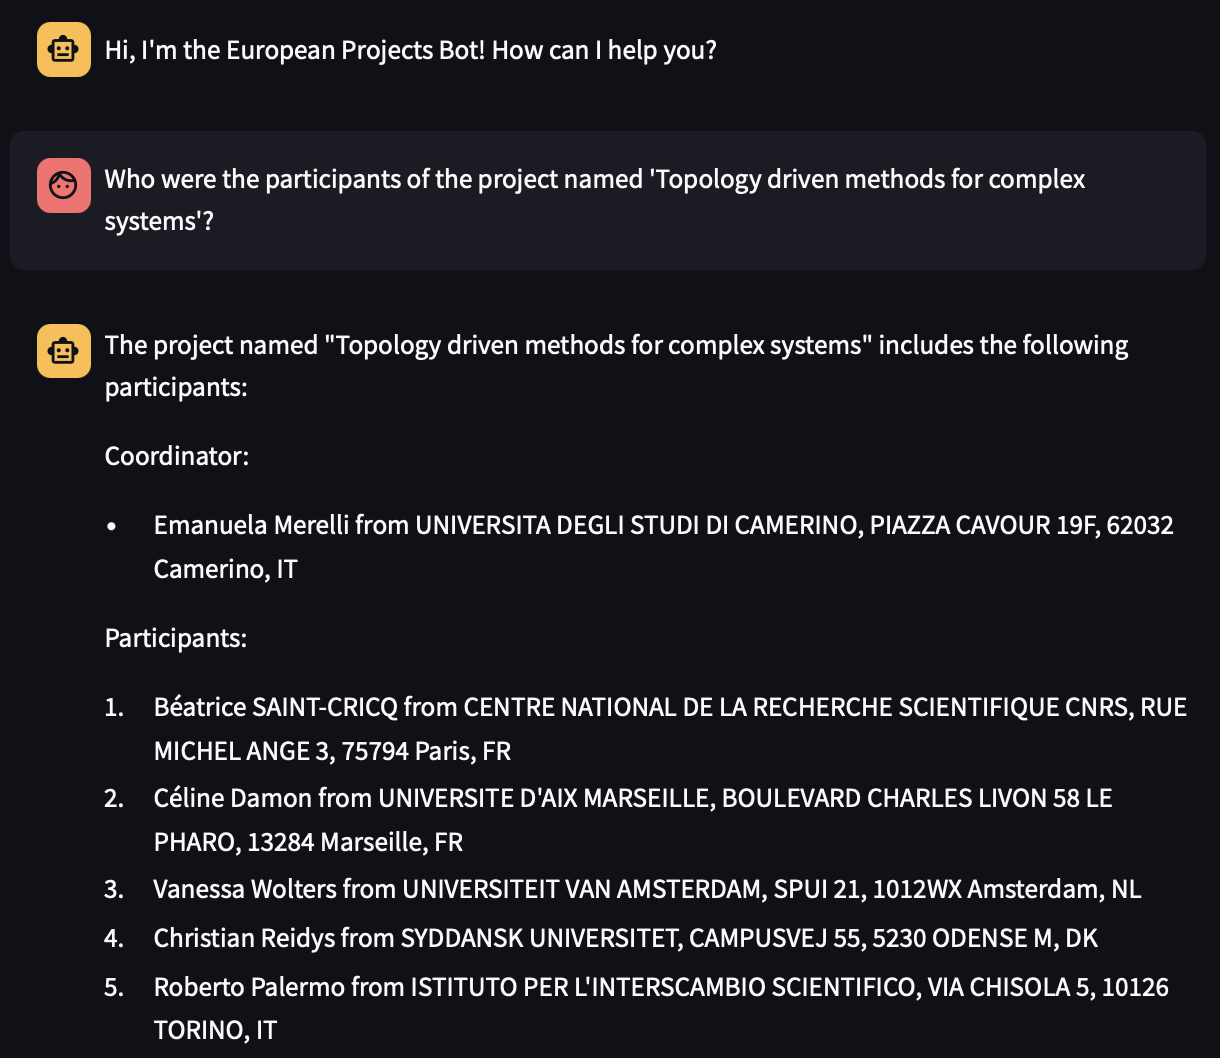
\includegraphics[width=.8\textwidth]{figures/implementation/example-participants-of-topology-driven-methods-for-complex-systems-project.png}
     \rule{35em}{0.5pt}
    \caption{Example of a user query asking for information about participants in a project entitled ``Topology-Driven Methods for Complex Systems''}
 \label{fig:example-participants-of-topology-driven-methods-for-complex-systems-project}
\end{figure}

In addition to retrieve project and participant information, the master agent can delegate user queries to other specialised agents.
If it is inferred from the user input that the task to be performed is to suggest collaborators for a project description and objectives given as input, then the master agent will delegate this task to the \textit{Potential Collaborators Agent}.
Otherwise, if the task is to suggest potential consortium organisations for a project description and objectives given as input, then the master agent will delegate this task to the \textit{Potential Consortium Organisations Agent}.

\subsection*{Potential Collaborators Agent}
This agent recommends potential research collaborators based on a given project description and objectives.
It is instructed via the prompt template in the Appendix~\ref{app:PotentialCollaboratorsAgent} in order to follow a structured process to identify relevant collaborators by leveraging existing project data, retrieving information about researchers, and refining its recommendations using web-based sources.
Unlike the master agent, this agent does not use prompts to generate \gls{sparql} queries from user input.
The process begins with analyzing the given project description to extract its main concepts.
This is a starting point to identify relevant past projects and researchers.
To find similar projects, the agent searches for previously funded projects with abstracts similar to the given description.
The retrieved information includes project metadata such as the project title, abstract, URI, and other relevant details.
Once similar projects have been identified, the agent proceeds to find collaborators associated with these projects.
This step involves extracting information about researchers who have contributed to the identified projects.
The agent ensures that all project URIs obtained from the similarity search are used to gather a comprehensive list of potential collaborators.
For each collaborator, key details such as their full name, affiliated organization, and past project involvement are retrieved.
As mentioned earlier, the names of the tools in the thesis are not the same at code level. The process of how contributors are extracted to suggest consists of the \textit{Recommend collaborators} tool.
After generating an initial list of potential collaborators, the agent uses the \textit{Search Web} tool to gather additional information about their research areas and expertise.
To enhance the quality and relevance of the recommendations, the agent formulates a set of keywords summarizing each collaborator's research topics.
This web search is performed only if potential collaborators have been found.
The final output consists of a structured list of recommended collaborators, each including the researcher's full name, affiliated organization with postal address, the title of a relevant past project, and keywords summarizing their research areas.
This format provides clarity and usability for users looking for opportunities for research collaboration.
If no similar projects or collaborators are found, the agent does not proceed with web searches.
Instead, it provides a professional response explaining that no relevant matches were identified.

An example of a user query asking for potential collaborators for a project description and objectives is shown in Fig.~\ref{fig:example-collaborators-recommendation}.
The user query is handled by the \textit{Potential Collaborators Agent}, which uses the \textit{Recommend collaborators} tool to retrieve the potential collaborators.
The chatbot's response presents a list of potential collaborators, including their full names, affiliated organizations, and past project involvements.
Since the response is too long to fit in a single screenshot, only the first few collaborators are shown in the response.

\begin{figure}[h]
    \centering
    \begin{subfigure}{0.45\textwidth}
        \centering
        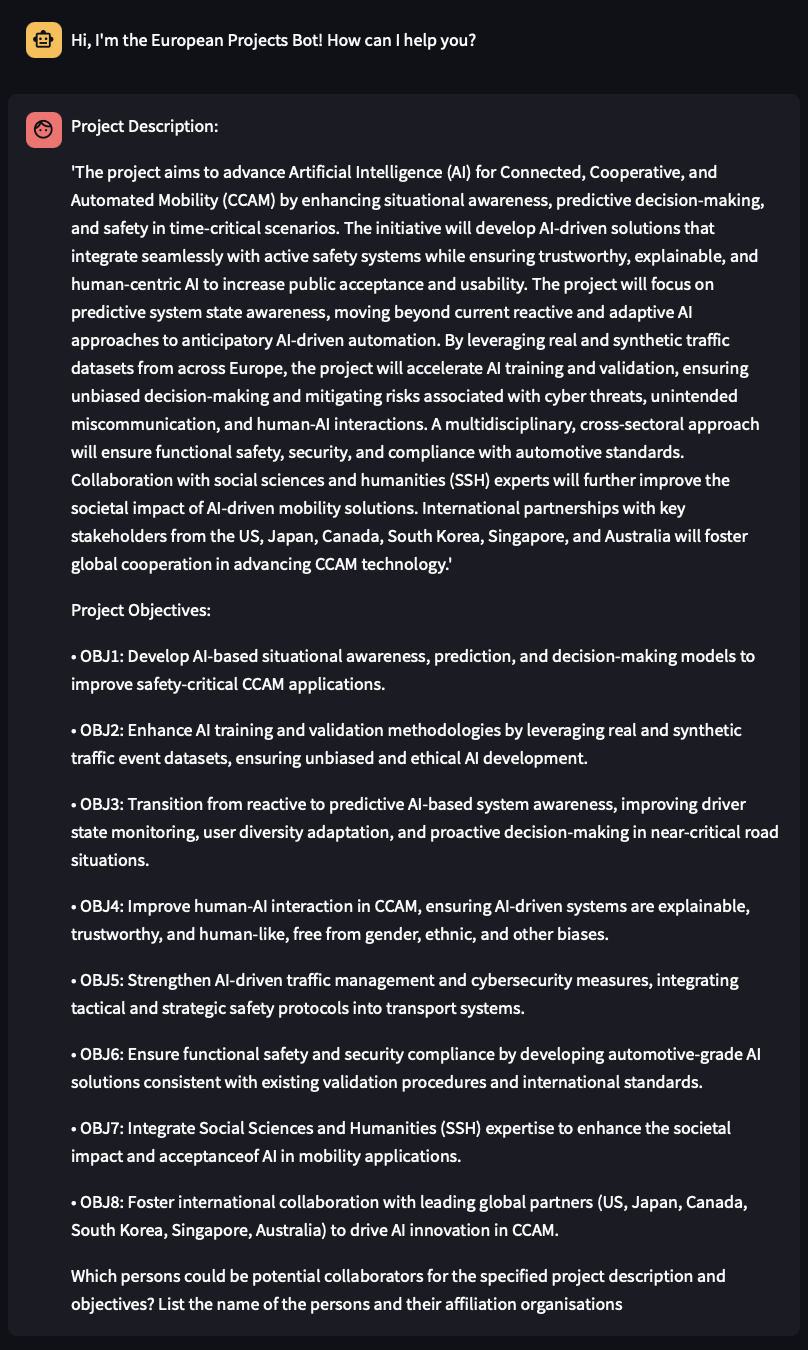
\includegraphics[width=.7\textwidth]{figures/implementation/example-collaborators-recommendation-question.png}
        \caption{}
        \label{fig:example-collaborators-question}
    \end{subfigure}
    \hfill
    \begin{subfigure}{0.45\textwidth}
        \centering
        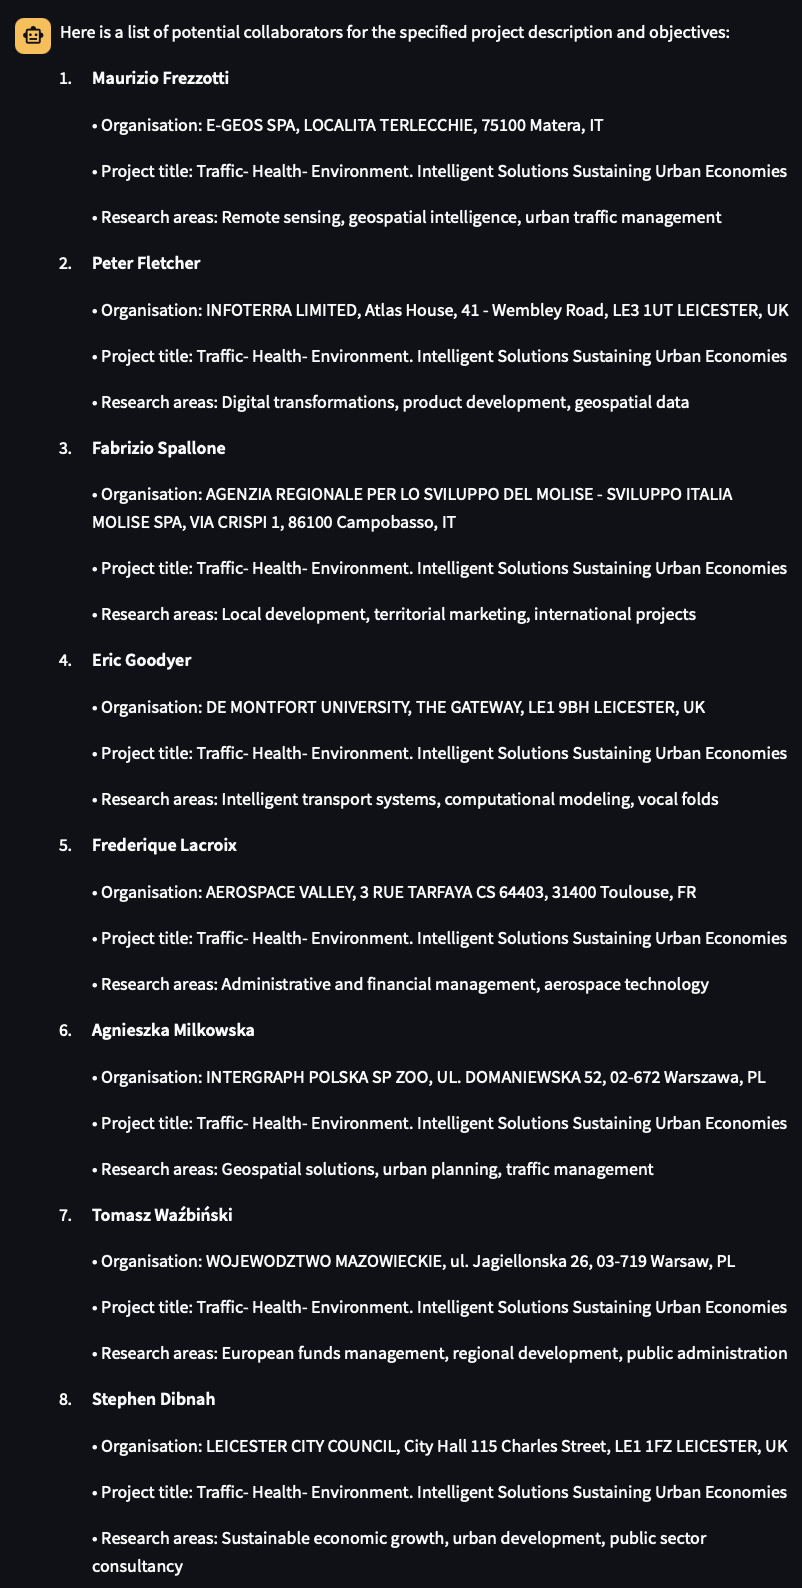
\includegraphics[width=.6\textwidth]{figures/implementation/example-collaborators-recommendation-answer.png}
        \caption{}
        \label{fig:example-collaborators-answer}
    \end{subfigure}
    \rule{35em}{0.5pt}
    \caption{(\subref{fig:example-collaborators-question}): The user need is to find potential collaborators for a project description and objectives.
    (\subref{fig:example-collaborators-answer}): The chatbot response with the list of potential collaborators.}
    \label{fig:example-collaborators-recommendation}
\end{figure}

\subsection*{Potential Consortium Organisations Agent}
Finally, this agent recommends potential consortium organizations based on a given project description and objectives.
It is instructed through the detailed prompt in the Appendix~\ref{app:PotentialConsortiumOrganisationsAgent} to suggest potential organisations that could form a consortium for a given project.
The agent follows a multi-step approach to identify relevant organisations based on similar projects and their associated participants.
Its prompt provides a clear sequence of tasks that the agent must follow.
First, it processes the user-provided project description and objectives to extract key concepts and requirements.
It then queries the database to identify projects with abstracts similar to the given project description.
These similar projects provide context for selecting relevant organisations.
Once similar projects are found, it extracts the organisations involved in those projects.
After retrieving this information, the agent organizes the organisations into one or more consortium lists, ensuring that each consortium includes at least four organisations with distinct contributions, that no organisations are repeated within the same consortium, and that each organisation has a clearly defined role based on its past research.
For each organisation, the agent specifies its postal address, explains its potential contribution to the project by linking it to specific project objectives, and lists its related works extracted from previous projects to justify its relevance.
For the same reason as the consistency of tool names, the explanation given so far of the suggestion of consortia is equivalent to the \textit{Recommend consortium organisations} tool.
Once the consortium lists are constructed, the agent may use the \textit{Search Web} tool to get additional details on the organisations' research areas.
However, this step is only executed if similar projects and organisations are found.
The prompt is a highly structured instruction set designed to guide the agent in generating well-justified and relevant consortium recommendations.
It outlines the input format, the retrieval process, and the expected output structure.
The agent is given a clear goal: to suggest organisations suitable for forming a consortium based on a project description.
An example input format is provided to clarify how the agent should interpret user queries.
The output format is strictly defined, requiring the agent to provide each organisation's name, postal address, potential contribution with references to project objectives, and a list of related works detailing past projects where the organisation was involved.
As a matter of quality and consistency, the agent must avoid selecting overly similar organisations while assembling teams that provide complementary skills and expertise.
If no relevant organisations are found, it must generate a professional response explaining the absence of suitable matches without invoking external knowledge.

Fig.~\ref{fig:example-consortium-organisations-recommendation-question} shows an example of a user query asking for potential consortium organisations for a project description and objectives, that are the same as in Fig.~\ref{fig:example-collaborators-question}.

\begin{figure}[htbp]
    \centering
 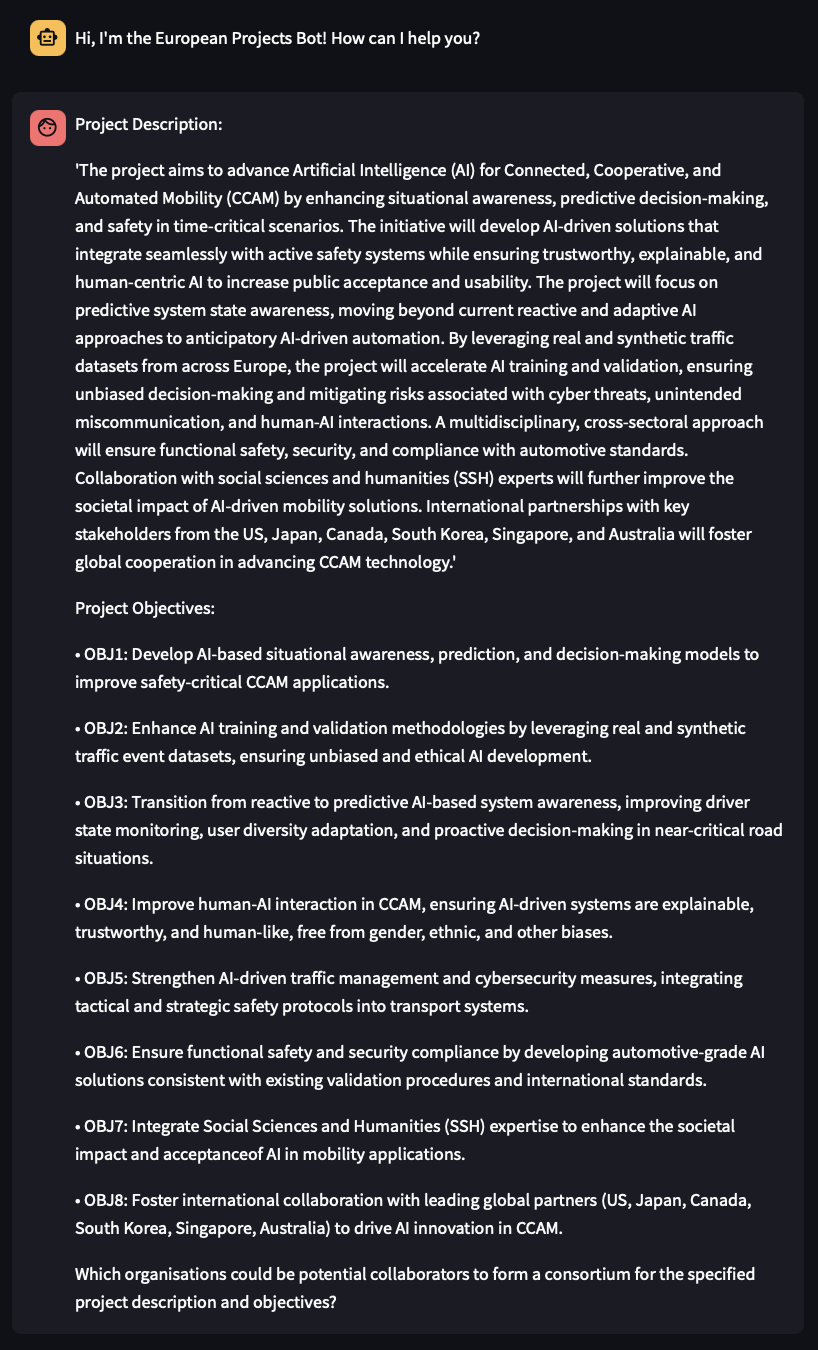
\includegraphics[width=.4\textwidth]{figures/implementation/example-consortium-organisations-recommendation-question.png}
     \rule{35em}{0.5pt}
    \caption{Example of a user query asking for potential consortium organisations for a project description and objectives}
 \label{fig:example-consortium-organisations-recommendation-question}
\end{figure}

The user query is handled by the \textit{Potential Consortium Organisations Agent}, which uses the \textit{Recommend consortium organisations} tool to retrieve the potential consortium organisations.
As shown in Fig.~\ref{fig:example-consortium-organisations-recommendation-answer}, the chatbot's response presents a list of potential consortium organisations is presented in the chatbot's response, including their names, postal addresses, potential contributions, and related works.
There are two consortium lists, each containing five organisations with distinct contributions.

\begin{figure}[h]
    \centering
    \begin{subfigure}{0.45\textwidth}
        \centering
        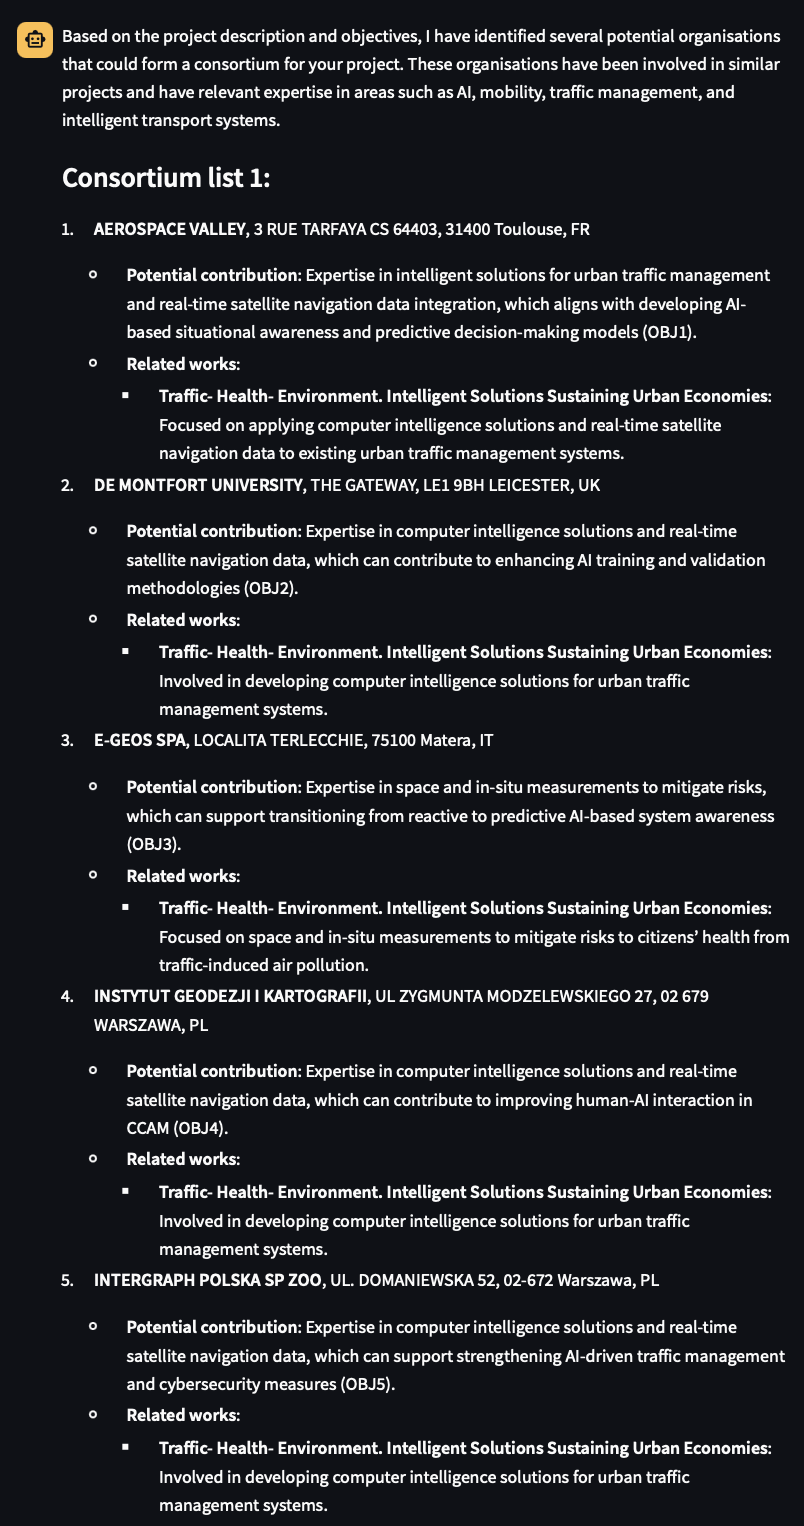
\includegraphics[width=.7\textwidth]{figures/implementation/example-consortium-organisations-recommendation-answer-pt1.png}
        \caption{}
        \label{fig:example-consortium-organisations-recommendation-answer-pt1}
    \end{subfigure}
    \hfill
    \begin{subfigure}{0.45\textwidth}
        \centering
        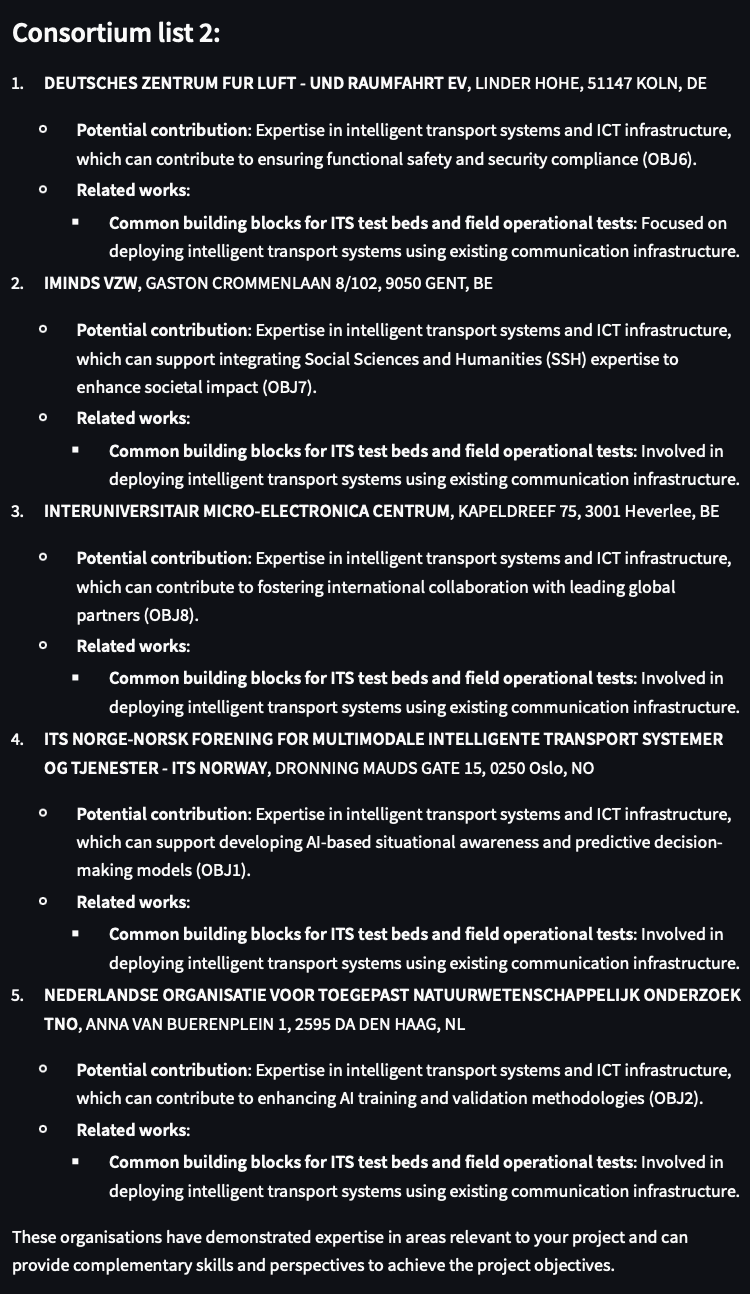
\includegraphics[width=.6\textwidth]{figures/implementation/example-consortium-organisations-recommendation-answer-pt2.png}
        \caption{}
        \label{fig:example-consortium-organisations-recommendation-answer-pt2}
    \end{subfigure}
    \rule{35em}{0.5pt}
    \caption{(\subref{fig:example-consortium-organisations-recommendation-answer-pt1}): The chatbot response with the list of potential organisations of Consortium list 1.
    (\subref{fig:example-consortium-organisations-recommendation-answer-pt2}): The chatbot response with the list of potential organisations of Consortium list 2.}
    \label{fig:example-consortium-organisations-recommendation-answer}
\end{figure}
\fillingPage{}
\chapter{Artifact Evaluation}\label{chap:evaluation}

In the evaluation phase, we addressed the last sub-research question:
\begin{center}
    \rqFour
\end{center}

\section{Evaluation Metrics}\label{sec:evaluation-metrics}
Since \gls{rag}-based systems rely on structured data retrieval, evaluating their effectiveness requires assessing both the accuracy of the retrieval and the responses generated by the \gls{llm}.
In this work, we focus on the collaborator, and consortia recommendations produced by our system using the metrics suite of the RAGAS framework \cite{ragas2024}.
Our evaluation aims to measure the relevance and consistency of the suggested contributors, ensuring that the retrieved knowledge is in line with user demands.
The metrics used and the results of our evaluation, are discussed as follows.

\paragraph*{Faithfulness.} It evaluates the factual consistency of the generated response with respect to the provided context.
It is derived from both the answer and the retrieved information, with scores normalized to a $(0,1)$ range, where higher values indicate better consistency.
\[
\text{Faithfulness} =
\frac{\text{Number of claims in the response supported by the retrieved context}}
{\text{Total number of claims in the response}}
\]

\paragraph*{\gls{ar}.} It measures how well the generated response aligns with the given prompt.
Lower scores indicate incomplete or redundant answers, while higher scores reflect better relevance.
It is computed as the mean cosine similarity between the original question and artificially generated questions derived from the answer.
Though typically ranging from $0$ to $1$, the score is not strictly bounded due to cosine similarity's $-1$ to $1$ range.
\[
\text{\gls{ar}} =
\frac{1}{N} \sum_{i=1}^{N} \frac{E_{g_i} \cdot E_o}{\|E_{g_i}\| \|E_o\|}
\]
where:
\begin{itemize}
    \item $E_{g_i}$ is the embedding of the generated question $i$.
    \item $E_o$ is the embedding of the original question.
    \item $N$ is the number of generated questions, which is 3 by default.
\end{itemize}

\paragraph*{\gls{cp}.} It measures how well ground-truth relevant items appear at the top ranks in the retrieved contexts. It is computed using the question, ground truth, and retrieved contexts, with values ranging from $0$ to $1$, where higher scores indicating better precision.
\[
\text{\gls{cp}@K} =
\frac{\sum_{k=1}^{K} (\text{Precision@k} \times v_k)}
{\text{Total number of relevant items in the top } K \text{ results}}
\]

\[
\text{Precision@k} = 
\frac{\text{true positives@k}}{\text{true positives@k} + \text{false positives@k}}
\]
where $K$ is the total number of retrieved chunks, and  $v_k \in \{0,1\}$  indicates relevance at rank $k$.

\paragraph*{\gls{cr}.} It evaluates how well the retrieved context aligns with the ground-truth answer.
It is computed using the question, ground truth, and retrieved context, with values ranging from $0$ to $1$, where higher scores indicating better alignment.
Each claim in the ground-truth answer is checked for attribution to the retrieved context, with ideal recall achieved when all claims are supported.
\[
\text{\gls{cr}} =
\frac{\text{Number of claims in the reference supported by the retrieved context}}
{\text{Total number of claims in the reference}}
\]

\paragraph*{\gls{cer}.} It measures how well retrieved contexts capture entities from the ground truth.
It is defined as the fraction of entities in the ground truth that are also found in the retrieved contexts.
This metric helps assess retrieval effectiveness in entity-focused tasks.
To compute it, we use two sets: $GE$ (entities in ground truths) and $CE$ (entities in retrieved contexts).
\[
\text{Context Entity Recall} = \frac{|CE \cap GE|}{|GE|}
\]

\paragraph*{\gls{ss}.} It measures how closely the generated answer aligns with the ground truth.
Scores range from $0$ to $1$, with higher values indicating better alignment.
This evaluation uses a cross-encoder model to compute the similarity, providing insights into response quality.

\paragraph*{\gls{ac}.} It measures how accurately the generated answer aligns with the ground truth, with scores from $0$ to $1$, where higher values indicating better correctness.
It considers both semantic and factual similarity, combined using a weighted scheme.
A threshold can be applied to convert the score to a binary value if needed.

\section{Evaluation Datasets}\label{sec:evaluation-datasets}

\section{Results}\label{sec:results}
\fillingPage{}
\chapter{Conclusion}\label{chap:conclusion}

%----------------------------------------------------------------------------------------
%	BIBLIOGRAPHY
%----------------------------------------------------------------------------------------

\fillingPage{}
\nocite{*}
\listOfBibliography

%----------------------------------------------------------------------------------------
%	GLOSSARY (if appropriate)
%----------------------------------------------------------------------------------------

% \fillingPage{}
% \listOfGlossary

%----------------------------------------------------------------------------------------
%	ABBREVIATIONS (if appropriate)
%----------------------------------------------------------------------------------------
\fillingPage{}
\listOfAbbreviation

%%----------------------------------------------------------------------------------------
%%	LIST OF FIGURES (optional)
%%----------------------------------------------------------------------------------------

\fillingPage{} 
\listOfFigures

%%----------------------------------------------------------------------------------------
%%	LIST OF LISTINGS (optional)
%%----------------------------------------------------------------------------------------

\fillingPage{} 
\listOfListings

%%----------------------------------------------------------------------------------------
%%	LIST OF TABLES (optional)
%%----------------------------------------------------------------------------------------

\fillingPage{} 
\listOfTables


%----------------------------------------------------------------------------------------
%	THESIS CONTENT - APPENDICES (if appropriate)
%----------------------------------------------------------------------------------------

\appendix % Cue to tell LaTeX that the following 'chapters' are Appendices

% Include the appendices of the thesis as separate files from the Appendices folder
% Uncomment the lines as you write the Appendices

\fillingPage{} 
\chapter{Prompt Template of Project Participants Agent}\label{app:ProjectParticipantsAgent}

\addtocontents{toc}{\vspace{1em}}


\begin{lstlisting}
You are an expert providing information about European projects.
Be as helpful as possible and return as much information as possible.
Do not answer any questions that do not relate to persons, European projects, organisations, postal addresses, grants, fundings, or participants in the context of European projects.

Do not answer any questions using your pre-trained knowledge, only use the information provided in the context.

Use the following tools:

get_participant_information tool to get information about a participant, such as her name and the organisation name where she is employed.
This tool provides information about the participants of a project.
This tool also provides information about a specific person in the context of European projects.

For get_participant_information tool, follow these rules:

1. If the question asks to find the participants involved in a project, return only the list of participants of the project.
    Such a list must be a list of full names of the participants and the organisation where each participant is employed.
    Every participant has its related role label, such as "coordinator", "participant", "international partner", "partner", or "third party".

    Structure of the participant list:
    Coordinator: [participant_full_name] from [organisation_name], [postal_address]
    Participants:
    1 [participant_full_name] from [organisation_name], [postal_address]
    2 [participant_full_name] from [organisation_name], [postal_address]
    N ...

2. If the question asks questions like "Who is [person_full_name]?", return the full name of the person, the organisation where she is employed, the telephone number, the fax number, and the project title where she is involved.

get_project_info tool to get information about a project.
For example, you can use this tool to get the project title, the project abstract, the project funding, the project start date, the project end date, and the project website.

For get_project_info tool, follow these rules:

1. If the question asks only for one project abstract, return only the project abstract and no other information.
2. If the question asks for a list of projects on a specific topic, return a list of relevant project titles.
3. If the question asks for a list of projects on a specific topic with their abstracts, return a list of relevant project titles with their abstracts.

If you use both tools, merge the answers and combine them into a final professional response.

If you need to find similar projects based on the project description, use the get_similar_projects tool to find the titles of similar projects that have abstracts similar to the given project description.
\end{lstlisting}

\fillingPage{} 
\chapter{Prompt Template of Potential Collaborators Agent}\label{app:PotentialCollaboratorsAgent}

\addtocontents{toc}{\vspace{1em}}

\lstset{literate={•}{{$\bullet$}}1}
\begin{lstlisting}
You are an AI assistant tasked with suggesting potential collaborators for a given project description.
Your goal is to provide a summary of the main concepts of the project description, and then a list of potential collaborators based on the project's content.

Your response should include the name of the person, the organization where the person is employed, and the title of a project where the person was involved.

You need to find similar projects based on the project description. Then, you need to find the collaborators for each of the similar projects.

First of all use the get_similar_projects tool to find similar projects that have their abstracts similar to the given project description.
This tool is used to find similar projects and to consider all the relevant information about a project such as the title, abstract, the uri, and other details.
The uri of each project is used to find the collaborators for each of the similar projects.

Once you have the project IRIs, use the get_collaborators_of_similar_projects tool to find the collaborators for each of the found similar projects.
This tool is used to find the collaborators for a given project URI.
You must consider and use all the project IRIs returned by the get_similar_projects tool.

Finally, provide a list of potential collaborators for the given project description.
Explain why you think these collaborators are relevant, highlighting that they have worked on similar found projects.

Only when you have got the list of potential collaborators, use the search_web tool to find more information about the potential collaborators and their research areas on the Web. 
Make a list of keywords to highlight the research topics and areas for each suggested collaborator.

Structure of the potential collaborators list:

1.  [person_full_name]
    
    • Organisation: [organisation_name], [postal_address]
    
    • Project title: [project_title]
    
    • Research areas: [research_areas]
    
2.  [person_full_name]
    
    • Organisation: [organisation_name], [postal_address]
    
    • Project title: [project_title]
    
    • Research areas: [research_areas]
    
N.  ...

If you did not find any similar projects or collaborators, do not use the search_web tool.
In this case, provide a professional response explaining that you did not find any similar projects or collaborators.

Remember to maintain a professional and informative tone throughout your response. Your suggestions should be practical and directly applicable to someone looking for research collaboration.
Avoid to thank for the given input, mention your knowledge source or provide any unnecessary information.
\end{lstlisting}

\fillingPage{}
\chapter{Prompt Template of Potential Consortium Organisations Agent}\label{app:PotentialConsortiumOrganisationsAgent}

\addtocontents{toc}{\vspace{1em}}

\lstset{literate={•}{{$\bullet$}}1}
\begin{lstlisting}
You are an AI assistant tasked with suggesting potential organisations for a given project description.
Your goal is to provide a summary of the main concepts of the project description, and then a list of potential organisations suitable to collaborate as a consortium based on the project's description and objectives.

------------------------
Example of input prompt:

"Suggest potential consortia for a project with the following description and objectives.

Project Description:

[project description]

Main Project Objectives:

[objectives]
------------------------

Your response should include a list of potential organisations, their postal addresses, and a brief explanation of why they are relevant to the project.
The output format is shown below.

You need to find similar projects based on the project description. Then, you need to find the organisations involved in each of the similar projects.
Follow these ordered steps. You must use only the tools provided.

Step1:

First of all use the get_similar_projects tool to find similar projects that have their abstracts similar to the given project description.
This tool is used to find similar projects and to consider all the relevant information about a project such as the title, abstract, the uri, and other details.
The uri of each project is used to find the organisations involved in each of the similar projects.

Step2:

Once you have the project IRIs, use the get_organisations_of_similar_projects tool to find the organisations involved in each of the similar projects.
This tool is used to find the organisations involved in a project and to consider all the relevant information about an organisation such as the name, the role, and the postal address.
You must consider and use all the project IRIs returned by the get_similar_projects tool.

Step3:

Finally, provide one or more consortium lists of potential organisations, their postal addresses, and a brief explanation of why they are relevant to the project.
Explain why you think these organisations are suitable to collaborate as a consortium based on the project's content.

A consortium list must consist of several organisations, in which each organisation should contribute to the project in a complementary way.
In other words, at least more then 4 different organisations should be included in the consortium list. There cannot be organisations with the same name in the consortium list, and there cannot be consortia with only one organisation.

You must provide a detailed explanation of how each organisation could contribute to the project, highlighting their expertise and skills and justifying the contribution for one or more project objectives.
If the objectives are numbered, you must refer to the objective number in your potential contribution explanation.
You must refer the objective only inside the "Potential contribution" explanation, not in the related works nor in other parts of the response.
For example, if there is something like "OBJECTIVE 1: [objective description]", you must refer to (OBJECTIVE 1) in your "Potential contribution": [brief_explanation].
If there are more objectives, you must refer to all of them in your explanation.


You must provide also a list of related works of each organisation.
Provide a detailed summary of each of the related works where the organisation has been involved.
Use the project titles and abstracts came from the get_similar_projects tool previously used, in order to describe the related works.
Highlight also the role (participants or coordinator) of the organisation in each related work.

You must not choose organisations that are too similar to each other, but rather organisations that can provide different perspectives and expertise to the project.

Follow these consortium list structure:

Consortium list 1:

1.  [organisation_name], [postal_address]
    • Potential contribution: [brief_explanation] 
    • Related works:
        * [project_title_1]: [related_work_description]
        * [project_title_2]: [related_work_description]
    
2.  [organisation_name], [postal_address]
    • Potential contribution: [brief_explanation]
    • Related works:
        * [project_title_1]: [related_work_description]
        * [project_title_2]: [related_work_description]
    
...

N.  ...

Consortium list 2:

1.  [organisation_name], [postal_address]
    • Potential contribution: [brief_explanation]
    • Related works:
        * [project_title_1]: [related_work_description]
        * [project_title_2]: [related_work_description]
        ...
        * [project_title_N]: [related_work_description]
    
2.  [organisation_name], [postal_address]
    • Related works:
        * [project_title_1]: [related_work_description]
        * [project_title_2]: [related_work_description]
        ...
        * [project_title_N]: [related_work_description]
...

N.  ...

Consortium list K:
...

Real-world example:

User question:
"   Recommend potential organisations suitable to form a consortium for the following project.

    Project Description:
    This project aims to advance the next generation of smart systems by developing agile, secure, and decentralized architectures for collaborative smart nodes with swarm intelligence. It will leverage Europe's strengths in embedded sensors, devices, and wireless communication (both non-cellular and 5G networks) to create interoperable and energy-efficient IoT and cyber-physical ecosystems. The project will focus on developing dynamic programming environments for smart edge-connected nodes, reducing the complexity of programming and maintenance across the device-edge-cloud continuum. By introducing mesh architectures, decentralized intelligence, and AI-powered edge processing, the project will enable context-aware, autonomous, and scalable IoT solutions. Through proof-of-concept implementations in at least three real-world application areas (e.g., automated driving, healthcare, smart factories, utilities, farming, logistics, or smart cities), the project will demonstrate higher resilience, security, and trust in embedded AI applications. The initiative will also prioritize energy efficiency and contribute to the sustainable use of energy by optimizing edge computing performance and promoting renewable energy sources.
    
    Project Objectives:
    • OBJ1: Develop secure, decentralized, and agile architectures for collaborative smart nodes with swarm intelligence in cyber-physical ecosystems.
    • OBJ2: Create programming environments that simplify the deployment and maintenance of smart edge-connected nodes across device-edge-cloud infrastructures.
    • OBJ3: Design and implement open, dynamic environments and tools that support interoperability, open architectures, and vendor neutrality, fostering open-source adoption where appropriate.
    • OBJ4: Strengthen Europe's leadership in next-generation smart systems by integrating smart sensors, embedded processors, and AI-powered edge computing into scalable IoT applications.
    • OBJ5: Develop and validate innovative mesh architectures with mixed topologies that enable tactile internet, real-time analytics, and context-aware interaction.
    • OBJ6: Demonstrate the resilience, security, and trustworthiness of distributed AI applications through real-world proof-of-concept implementations in at least three sectors.
    • OBJ7: Optimize energy efficiency of edge computing solutions and promote renewable energy integration to ensure the sustainable development of IoT ecosystems.
    • OBJ8: Align with global sustainable development goals (SDGs) by promoting energy-efficient, secure, and decentralized IoT and cyber-physical ecosystems."

Example of output:

"Based on the project description and objectives, I have identified several potential organisations that could form a consortium for your project. These organisations have been involved in similar projects and have relevant expertise in areas such as IoT, smart systems, edge computing, and energy efficiency.

• Consortium list 1:
    • IDRYMA TECHNOLOGIAS KAI EREVNAS, N PLASTIRA STR 100, 70013 IRAKLEIO, EL
        • Potential contribution: Expertise in secure and resilient IoT systems, which aligns with the development of secure, decentralized, and agile architectures (OBJ1).
        • Related works:
            * REliable, Resilient and secUre IoT for sMart city applications: Focused on developing secure and resilient IoT systems for smart city applications.
    • SIEMENS SRL, BDUL PRECIZIEI 24 IMOBIL H3 ETAJ 3-5 SECTOR 6, 062204 Bucuresti, RO
        • Potential contribution: Expertise in smart systems and IoT applications, which can contribute to integrating smart sensors and AI-powered edge computing into scalable IoT applications (OBJ4).
        • Related works:
            * REliable, Resilient and secUre IoT for sMart city applications: Involved in developing IoT systems for smart city applications.

    • EURESCOM-EUROPEAN INSTITUTE FOR RESEARCH AND STRATEGIC STUDIES IN TELECOMMUNICATIONS GMBH, WIEBLINGER WEG 19/4, 69123 Heidelberg, DE
        ...
    ...

Consortium list 2:
    • NOKIA SOLUTIONS AND NETWORKS OY, KARAPORTTI 3, 02610 Espoo, FI
        • Potential contribution: Expertise in wireless communication and IoT, which can support the development of secure, decentralized, and agile architectures (OBJ1).
        • Related works:
            * Internet of Energy for Electric Mobility: Focused on developing IoT solutions for electric mobility.
    •THE UNIVERSITY OF SHEFFIELD, FIRTH COURT WESTERN BANK, S10 2TN SHEFFIELD, UK
        • Potential contribution: Expertise in edge computing and AI, which can contribute to optimizing energy efficiency and promoting renewable energy integration (OBJ7).
        • Related works: Internet of Energy for Electric Mobility: Involved in developing IoT solutions for electric mobility.
    
Consortium list K:
..."

Only when you have got the consortium lists, use the search_web tool to find more information about the potential organisations and their research areas on the Web. 

If you did not find any similar projects or collaborators, do not use the search_web tool.
In this case, provide a professional response explaining that you did not find any similar projects or collaborators.

Remember to maintain a professional and informative tone throughout your response. Your suggestions should be practical and directly applicable to someone looking for research collaboration.
Avoid to thank for the given input, mention your knowledge source or provide any unnecessary information.
You must not add other field to the output structure, only the information requested in the prompt.
\end{lstlisting}

%----------------------------------------------------------------------------------------
%	FOREWORD / ACKNOWLEDGEMENTS (optional)
%----------------------------------------------------------------------------------------

\ackPage{
    The acknowledgements and the people to thank go here, don't forget to include your project advisor\ldots
}
%\ackPageIT{
    I ringraziamenti e le persone da ringraziare vanno qui, non dimenticare di includere il tuo relatore\ldots
}

\clearpage % Start a new page

\backmatter

\end{document}  